\documentclass[a4paper,10pt
,draft
%, final
]{article}%


% ---- Commands on draft --------

\usepackage[dvipsnames]{xcolor}% adds colors
\usepackage{ifdraft}
\ifdraft{
  \color[RGB]{63,63,63}
%  \pagecolor[RGB]{220,220,204}
  \usepackage[notref]{showkeys}
  \usepackage{geometry}
  \usepackage{todonotes}
}
{
  \usepackage[margin=1in]{geometry}
  \usepackage[fontsize=12pt]{scrextend}
  \usepackage[disable]{todonotes}
}

\pdfcompresslevel=0
\pdfobjcompresslevel=0

%\usepackage{xr-hyper}
\usepackage[pagebackref, colorlinks, citecolor=PineGreen, linkcolor=PineGreen]{hyperref}
\hypersetup{
  final,
  pdftitle={Equivariant dendroidal sets and simplicial operads},
  pdfauthor={Bonventre, P. and Pereira, L. A.},
  linktoc=page
}

%\externaldocument*[HGOP-]{HtpyGOp} % cite using names from other half

\usepackage{amsmath, amsthm}% {amsfonts, amssymb}

% ------ New Characters --------------------------------------

\usepackage[latin1]{inputenc}%
\usepackage{MnSymbol}
\DeclareMathAlphabet\mathbb{U}{msb}{m}{n}
%\usepackage{stmaryrd}
%\usepackage{upgreek}
\usepackage{mathrsfs}
% \usepackage[T1]{fontenc}
% \usepackage[english]{babel}
% \usepackage{fouriernc}
% \DeclareMathAlphabet{\mathscr}{U}{mathrsfs}{m}{n}`

\usepackage[normalem]{ulem}%
\usepackage{dsfont}%
\usepackage{bbm}%


%----- Enumerate ---------------------------------------------
% \usepackage{paralist} % for inparaenum
% \usepackage{enumerate}%
\usepackage[inline,shortlabels]{enumitem}%


% ---------- Page Typesetting ----------
\usepackage[final]{microtype}
\usepackage{relsize}

%-------- Tikz ---------------------------

\usepackage{tikz}%
\usetikzlibrary{matrix,arrows,decorations.pathmorphing,
cd,patterns,calc}
\tikzset{%
  treenode/.style = {shape=rectangle, rounded corners,%
                     draw, align=center,%
                     top color=white, bottom color=blue!20},%
  root/.style     = {treenode, font=\Large, bottom color=red!30},%
  env/.style      = {treenode, font=\ttfamily\normalsize},%
  dummy/.style    = {circle,draw,inner sep=0pt,minimum size=2mm}%
}%

\usetikzlibrary[decorations.pathreplacing]





% ----- Labels Changed? --------

\makeatletter

\def\@testdef #1#2#3{%
  \def\reserved@a{#3}\expandafter \ifx \csname #1@#2\endcsname
  \reserved@a  \else
  \typeout{^^Jlabel #2 changed:^^J%
    \meaning\reserved@a^^J%
    \expandafter\meaning\csname #1@#2\endcsname^^J}%
  \@tempswatrue \fi}

\makeatother

%%%%%%%%%%%%%%%%%%%%%%%%% INTERNAL REFERENCES %%%%%%%%%%%%%%%%%%%%%%%%%%%%%%%%%%%

\numberwithin{equation}{section} 
\numberwithin{figure}{section}

\usepackage{mathtools}
\mathtoolsset{showonlyrefs,showmanualtags} % Only number equations which are referenced with eqref


% ------- New Theorems/ Definition/ Names-----------------------

 % \theoremstyle{plain} % bold name, italic text
\newtheorem{theorem}[equation]{Theorem}%
\newtheorem*{theorem*}{Theorem}%
\newtheorem{lemma}[equation]{Lemma}%
\newtheorem{proposition}[equation]{Proposition}%
\newtheorem{corollary}[equation]{Corollary}%
\newtheorem{conjecture}[equation]{Conjecture}%
\newtheorem*{conjecture*}{Conjecture}%
\newtheorem{claim}[equation]{Claim}%

%%%%%% Fancy Numbering for Theorems
\newtheorem{innercustomgeneric}{\customgenericname}
\providecommand{\customgenericname}{}
\newcommand{\newcustomtheorem}[2]{%
  \newenvironment{#1}[1]
  {%
   \renewcommand\customgenericname{#2}%
   \renewcommand\theinnercustomgeneric{##1}%
   \innercustomgeneric
  }
  {\endinnercustomgeneric}
}

\newcustomtheorem{customthm}{Theorem}
\newcustomtheorem{customcor}{Corollary}
%%%%%%%%%%%%%

\theoremstyle{definition} % bold name, plain text
\newtheorem{definition}[equation]{Definition}%
\newtheorem*{definition*}{Definition}%
\newtheorem{example}[equation]{Example}%
\newtheorem{remark}[equation]{Remark}%
\newtheorem{notation}[equation]{Notation}%
\newtheorem{convention}[equation]{Convention}%
\newtheorem{assumption}[equation]{Assumption}%
\newtheorem{exercise}{Exercise}%


% %%%%%%%%%%%%%%%%%%%%%%%%%%%%%%%%%%%%%%%%%%%%%%%%%%%%%%%%%%%%%%%%%%%%%%%%%%%%%%%%
% ------------------------------ COMMANDS ------------------------------

% ---------- macros

\newcommand{\set}[1]{\left\{#1\right\}}%
\newcommand{\sets}[2]{\left\{ #1 \;|\; #2\right\}}%
\newcommand{\longto}{\longrightarrow}%
\newcommand{\into}{\hookrightarrow}%
\newcommand{\onto}{\twoheadrightarrow}%

\usepackage{harpoon}
\newcommand{\vect}[1]{\text{\overrightharp{\ensuremath{#1}}}}


% ---------- operators

\newcommand{\Sym}{\ensuremath{\mathsf{Sym}}}%
\newcommand{\Fin}{\mathsf{F}}%
\newcommand{\Set}{\ensuremath{\mathsf{Set}}}
\newcommand{\Top}{\ensuremath{\mathsf{Top}}}
\newcommand{\sSet}{\ensuremath{\mathsf{sSet}}}%
\newcommand{\Cat}{\mathsf{Cat}}
\newcommand{\sCat}{\mathsf{sCat}}
\newcommand{\Op}{\mathsf{Op}}%
\newcommand{\sOp}{\ensuremath{\mathsf{sOp}}}%
\newcommand{\fgt}{\ensuremath{\mathsf{fgt}}}%
\newcommand{\dSet}{\mathsf{dSet}}
\newcommand{\Fun}{\mathsf{Fun}}
\newcommand{\Fib}{\mathsf{Fib}}
\newcommand{\Alg}{\mathsf{Alg}}
\newcommand{\Kl}{\mathsf{Kl}}



\DeclareMathOperator{\hocmp}{hocmp}%
\DeclareMathOperator{\cmp}{cmp}%
\DeclareMathOperator{\hofiber}{hofiber}%
\DeclareMathOperator{\fiber}{fiber}%
\DeclareMathOperator{\hocofiber}{hocof}%
\DeclareMathOperator{\hocof}{hocof}%
\DeclareMathOperator{\holim}{holim}%
\DeclareMathOperator{\hocolim}{hocolim}%
\DeclareMathOperator{\colim}{colim}%
\DeclareMathOperator{\Lan}{Lan}%
\DeclareMathOperator{\Ran}{Ran}%
\DeclareMathOperator{\Map}{Map}%
\DeclareMathOperator{\Id}{Id}%
\DeclareMathOperator{\mlf}{mlf}%
\DeclareMathOperator{\Hom}{Hom}%
\DeclareMathOperator{\Ho}{Ho}
\DeclareMathOperator{\Aut}{Aut}%
\DeclareMathOperator{\Stab}{Stab}
\DeclareMathOperator{\Iso}{Iso}
\DeclareMathOperator{\Ob}{Ob}

% ---------- shortcuts

\newcommand{\F}{\ensuremath{\mathcal F}}
\newcommand{\V}{\ensuremath{\mathcal V}}
\newcommand{\Q}{\ensuremath{\mathcal Q}}
\renewcommand{\O}{\ensuremath{\mathcal O}}
\renewcommand{\P}{\ensuremath{\mathcal P}}
\newcommand{\C}{\ensuremath{\mathcal C}}
\newcommand{\A}{\ensuremath{\mathcal A}}

\newcommand{\del}{\partial}%

\newcommand{\ki}{\chi}
\newcommand{\ksi}{\xi}
\newcommand{\Ksi}{\Xi}

\newcommand{\lltimes}{\underline{\ltimes}}

% detecting $\V$-categories:

\newcommand{\I}{\mathbb I}
\newcommand{\J}{\mathbb J}
\newcommand{\1}{\ensuremath{\mathbbm 1}}%{\ensuremath{\mathbb{id}}} %\eta

% lazy shortcuts

\newcommand{\SC}{\Sigma_{\mathfrak C}}
\newcommand{\OC}{\Omega_{\mathfrak C}}
\newcommand{\UV}{\underline{\mathcal V}}
\newcommand{\UC}{\underline{\mathfrak C}}











% %%%%%%%%%%%%%%%%%%%%%%%%%%%%%%%%%%%%%%%%%%%%%%%%%%%%%%%%%%%%%%%%%%%%%%%%%%%%%%%%%%%%%%%%%%%%%%%%%%%%
% ------------------------------ MAIN BODY ------------------------------

% ---- Title --------

\title{Equivariant dendroidal sets and simplicial operads}

\author{Peter Bonventre, Lu\'is A. Pereira}%

\date{\today}


% ---- Document body --------

\begin{document}

\maketitle

\begin{abstract}
      Things and stuff
\end{abstract}

\tableofcontents


\section{Introduction}



\subsection{Main Results}



\begin{theorem}\label{QE THM}
The adjunction
\[
W_! \colon \dSet^G \rightleftarrows \sOp^G \colon hcN
\] is a Quillen equivalence.
\end{theorem}


{\color{blue} HERE}



\begin{theorem}
	Tame model structure exists, and we have Quillen equivalences
	$\mathsf{PreOp}^G \leftrightarrows \mathsf{PreOp}^G_{tame} \rightleftarrows \sOp^G$.
\end{theorem}





\subsection{Whatever}




\begin{example}
      \label{COTENS_EX}
      Letting $\mathcal{O} \in \mathsf{sOp}$ be a simplicial colored operad
      and $K \in \mathsf{sSet}$,
      one has a pointwise simplicial cotensoring
      $\{K,\O\}_{\mathsf{F}} \in \mathsf{sOp}$
      given by
      $\{K,\O\}_{\mathsf{F}}(\vect C) = 
      \left(\O(\vect C)\right)^K$
      for each signature $\vect C$.
      %
      $\{K,-\}_{\mathsf{F}}\colon \mathsf{sOp} \to \mathsf{sOp}$
      is then a fibered right adjoint which preserves pullback arrows,
      and thus the corresponding adjunction is also fibered.
\end{example}

\begin{example}
      \label{TENS_EX}
      We warn that the tensoring left adjoint, denoted $(-) \otimes_{\Fin} K: \sOp \to \sOp$, is in general \textit{not} levelwise.
      However, for $C \in \Sigma$, we have the following:
      \begin{enumerate}[label = (\roman*)]
      \item $\Omega(C) \otimes_\Fin K(\vect D) = \Omega(C)(\vect D) \times K$,
      \item $\Omega(C) \otimes_\Fin K = (\mathbb F_{\Set} \Sigma_\bullet[C]) \otimes_\Fin K = \mathbb F_{\sSet} (\Sigma_\bullet[C] \cdot K)$.
      \item $\Hom_{\Op}(\Omega(C) \otimes_\Fin K, \O) = \displaystyle\coprod_{\mbox{$C$-profiles $\vect C$}} \Hom_{\sSet}(K, \O(\vect C)),$
      \item The set of squares on the left below are in bijection with the set of squares are the right, where $\vect C$ runs over all $C$-profiles.
            \begin{equation}
                  \begin{tikzcd}
                        \Omega(C) \otimes_\Fin K \arrow[r] \arrow[d, "u"']
                        &
                        \O \arrow[d, "F"]
                        & %----------
                        K \arrow[r] \arrow[d, "u"']
                        &
                        \O(\vect C) \arrow[d, "{F(\vect C)}"]
                        \\
                        \Omega(C) \otimes_\Fin L \arrow[r]
                        &
                        \P
                        & % ----------
                        L \arrow[r]
                        &
                        \P(F(\vect C))
                  \end{tikzcd}
            \end{equation}
      \end{enumerate}
\end{example}




\newpage

\section{Review of previous work}

In this mostly expository section, we recall the main features of the model structures necessary for the later sections.
Full details and discussion can be found in \cite{Per18}, \cite{BP_edss}.

\[
      \begin{tikzcd}
            \mathsf{PreOp}^G \ar{d}[swap]{\gamma^{\**}}&
            \mathsf{sOp}^G \ar{l}[swap]{N} \ar{d}{hcN}
            \\
            \mathsf{sdSet}^G &
            \mathsf{dSet}^G \ar{l}{c_{!}}
      \end{tikzcd}
\]


\subsection{Equivariant trees}

cat

\begin{definition}
      $\Phi_\bullet^0 \subseteq \Phi_\bullet$
\end{definition}


\subsection{Equivariant dendroidal sets}
\label{EDS_SEC}

We begin with a brief overview of $G$-trees and equivariant dendroidal sets, whose discovery/definition is central and motivating for this entire project.

\begin{definition}
      The category $\Omega_G$ of \textit{$G$-trees} is the category of indecomposable forests with $G$-action.
      Equivalently, an object $T \in \Omega_G$ can be described as any of the following:
      \begin{enumerate}[label = (\roman*)]
      \item A collection $T = (T_i)_{i \in R}$ of trees in $\Omega$, together with a compatible $G$-action on the whole system.
      \item A functor $T: G \ltimes R \to \Omega$ for $R = \mathbf R(T)$ the transitive $G$-set of \textit{roots} of $T$.
      \item An induction $T \simeq G \cdot_H T_e$ for some $T_e \in \Omega^H$ and $H \leq G$.
      \item A quotient $T \simeq G \cdot U / \Gamma$ for some $U \in \Omega$ and graph subgroup $\Gamma \leq G \times \Aut(U)$.
            % \item The quotient $T \simeq (G \cdot T_e) / N$ for $N$ the graph of the homomorphism $H \to \Aut(T_e)$ encoding the $H$-action.
      \end{enumerate}
\end{definition}

We consider the na\"ive presheaf category 
$
\dSet^G = \Fun(G \times \Omega^{op}, \Set),
$
of \textit{equivariant dendroidal sets}.
There is a natural inclusion
\[
      \Omega[-] \colon \Omega_G \to \dSet^G,
      \qquad
      \Omega[T] = \coprod \Omega[T_i] \simeq G \cdot_H \Omega[T_e].
      % \simeq \left(G \cdot \Omega[T_e] \right) / N
\]
extending the Yoneda embedding $\Omega \times G \into \dSet^G$.
Even though the presheaf category is na\"ive, this functor allows us to see genuine equivariant information recorded by $G$-trees
and build a more ``genuine'' model structure.
To begin, we make the following definitions (see \cite[\S 6]{Per18}).

\begin{definition}
      For $T \in \Omega_G$, let $\partial \Omega[T]$ denote the \textit{boundary}
      \[
            \partial \Omega[T] = \coprod \partial \Omega[T_i] \simeq G \cdot_H \partial \Omega[T_e].
            % \simeq \left(G \cdot \partial \Omega[T_e] \right) / N.
      \]
      The \textit{boundary inclusions} are maps in $\dSet^G$ of the form
      \[
            \partial \Omega[T] \to \Omega[T] =
            \coprod \big( \partial \Omega[T_i] \to \Omega[T_i]\big) \simeq
            G \cdot_H \big( \partial \Omega[T_e] \to \Omega[T_e] \big).
            % \simeq
            % \left( G \cdot \left( \partial \Omega[T_e] \into \Omega[T_e] \right) \right) / N.
      \]
\end{definition}

\begin{definition}
      Given $T \in \Omega_G$ and $e \in E(T)$, the associated \textit{$G$-inner horn} is the sub presheaf
      \begin{equation}
            \label{GINNERHORN_EQ}
            \Lambda^{Ge}[T] \into \partial \Omega[T] \into \Omega[T],
            \qquad
            \Lambda^{Ge}[T] = \amalg \Lambda^{H_i e}{T_i} \simeq G \cdot_H \Lambda^{He}[T_e].
            % \simeq \left(G \cdot \Lambda^{He}[T_e] \right) / N.
      \end{equation}
      The \textit{generating $G$-inner horn inclusion} are maps in $\dSet^G$ of the form
      \begin{equation}
            \label{GENIHI_EQ}
            \Lambda^{Ge}[T] \to \Omega[T]
      \end{equation}
      for $T \in \Omega_G$ and $e \in E(T)$.

      A presheaf $X$ is called a \textit{$G$-$\infty$-operad} if $X \to \**$ has the right lifting property with respect to all generating $G$-inner horn inclusions.
\end{definition}

\begin{definition}
      The class of \textit{$G$-normal monomorphisms}
      is the smallest saturated\footnote{A class of maps is \textit{saturated} if it is closed under pushouts, retracts, and transfinite compositions.}
      class of maps containing the boundary inclusions $\partial \Omega[T] \into \Omega[T]$.
      A map is called a \textit{trivial fibration} if it has the right lifting property with respect to the $G$-normal monomorphisms.
      
      The class of \textit{$G$-inner anodyne extensions} is the smallest saturated class of maps containing the generating $G$-inner horn inclusions.
\end{definition}

These two classes of maps form the basis of a model structure on $\dSet^G$.

\begin{theorem}[{\cite[Thm 2.1, Thm 8.22]{Per18}}]
      There exists a model structure on $\dSet^G$ such that
      \begin{itemize}
      \item cofibrations are $G$-normal monomorphisms,
      \item fibrant objects are $G$-$\infty$-operads,
      \item fibrations between fibrant objects are precisely the maps $X \to Y$ such that the functors associated to each of the fixed-point homotopy categories $\tau j^{\**}(X^H \to Y^H)$ are categorical fibrations for all $H \leq G$.
      \item weak equivalences are the smallest class of maps closed under 2-out-of-3 which
            contains the $G$-inner anodyne extensions and trivial fibrations.
      \end{itemize}
\end{theorem}


These results will be applied in Proposition \ref{W!_COF_PROP}, the main result necessary to prove that $W_!$ is left Quillen.








\subsection{Equivariant simplicial operads}

We will denote by $\mathsf{sOp}$ the category of \textit{colored simplicial operads}, also know as \textit{simplicially enriched multicategories},
and $\mathsf{sOp}^G$ the category of $G$-objects in $\sOp$.

\begin{definition}
      Let $\mathcal{V}$ be a category.
      The category $\mathsf{Sym}_\bullet(\mathcal{V})$ of
      \textit{symmetric sequences on $\mathcal{V}$} 
      (on all colors) is the category with:
      \begin{itemize}
      \item objects given by pairs $(\mathfrak C, X)$ with
            $\mathfrak{C} \in \mathsf{Set}$ a set of colors and
            $X \colon \Sigma_{\mathfrak{C}}^{op} \to \mathcal{V}$ a functor;
      \item arrows $(\mathfrak C, X) \to (\mathfrak D, Y)$ given by a map 
            $\varphi \colon \mathfrak{C} \to \mathfrak{D}$ of colors and a natural transformation $X \Rightarrow Y \varphi$ as below.
            \begin{equation}
                  \label{SYMSEQMAP_EQ}
                  \begin{tikzcd}[row sep = tiny, column sep = 45pt]
                        \Sigma_{\mathfrak{C}}^{op} \arrow[dr, "X"{name=U}] 
                        \arrow{dd}[swap]{\varphi}
                        \\
                        & \mathcal{V}
                        \\
                        |[alias=V]| \Sigma_{\mathfrak{D}}^{op} \arrow[ur, "Y"']
                        \arrow[Leftarrow, from=V, to=U,shorten >=0.25cm,shorten <=0.25cm]
                  \end{tikzcd}
            \end{equation}
      \end{itemize}
\end{definition}

\begin{definition}
      Describe.
\end{definition}

\subsubsection{$\Sigma$-cofibrancy}


\subsubsection{Free operads generated by trees}

Several important examples of (equivariant) operads are generated by ($G$)-trees.
We begin by recalling some constructions from \cite[\S 2.3.1]{BP_HGOP} % {REPFUN_SEC}.

Given $\vect C \in \Sigma_{\mathfrak C}$, we have a representable functor $\Sigma_{\mathfrak C}[\vect C] = \Sigma_{\mathfrak C}^{op}(\vect C, -)$ in $\Sym_{\mathfrak C}$..
More generally, for any $\mathfrak C$-colored forest $\vect F$, we define
\[
      \Sigma_{\mathfrak C}[\vect F] = \sideset{}{^{\mathfrak C}}\coprod_{v \in \boldsymbol{V}(F)} \Sigma_{\mathfrak C}[\vect F_v],
\]
where we highlight that the coproduct $\amalg^{\mathfrak C}$ is fibered, i.e. takes place in $\Sym_{\mathfrak C}$ rather than $\Sym_\bullet$.
This extends to functors
\[
      \Phi_\bullet^0 \xrightarrow{\Sigma_\bullet[-]} \Sym_\bullet
      \qquad
      \Phi_\bullet^{0,G} \xrightarrow{\Sigma_\bullet[-]} \Sym_\bullet^G
\]
which are fibered over $\Set$ and $\Set^G$, respectively.

We also recall the \textit{tautological coloring} functor $(-)^\tau \colon \Phi \to \Phi_{\bullet}$
which sends $F \in \Phi$ to $F^\tau \in \Phi_{\boldsymbol{E}(T)}$,
where $F^\tau = (F,\mathfrak t)$ is the underlying forest $F$ together with the identity coloring map $\mathfrak t \colon \boldsymbol{E}(T) \xrightarrow{=} \boldsymbol{E}$.
We abbreviate $\Sigma_\tau[F] := \Sigma_{\boldsymbol{E}(F)}[F^\tau]$.

We may now construct our free operads generated by trees.

\begin{definition}
      \label{OT_DEF}
      Fix $T \in \Omega_G$.
      We define $\Omega(T) \in \Op_\bullet^G$ to be the free operad
      \[
            \Omega(T) := \mathbb F \Sigma_\tau[T].
      \]
\end{definition}
Explicitly, $\Omega(T)$ has colors $\mathfrak C = \boldsymbol{E}(T)$ the set of edges, and
for any $\boldsymbol{E}(T)$-signature $\vect C$, we have
\begin{equation}
      \label{OMEGADEF_EQ}
      \Omega(T)(\vect C) =
      \begin{cases}
            \** \qquad & \mbox{there exists $C \xrightarrow{\phi} T$ in $\Omega$ such that $\partial \phi = \vect C$}
            \\
            \varnothing & \text{else,}
      \end{cases}
\end{equation}
where $\partial \phi$ is the $\mathbf E(U)$-signature $(\phi(1), \phi(2), \dots, \phi(n); \phi(0))$
given by the (ordered) image of the edges of $C$.
\todo[inline]{profile of a map? is this used in other places?}

This extends to a fully-faithful functor\footnote{In fact, non-equivariantly this inclusion is used as a \textit{definition} of the category $\Omega$} $\Omega_G \into \Op_\bullet^G$.


% \begin{remark}
%       We have an additional fully-faithful inclusion $\Omega_G \into \dSet^G$ (e.g. \cite[Notation 5.56]{Per18}), sending $T = (T_i) \in \Omega_G$ to
%       $\Omega[T] := \coprod_{i}\Omega[T_i]$.
%       These two functors assemble to give a nerve-realization adjunction as below.
% \begin{equation}
%       \label{DSETADJ_EQ}
%       \begin{tikzcd}
%             \dSet^G \arrow[r, shift left, "\tau"]
%             &
%             \Op_\bullet^G \arrow[l, shift left, "N"]
%       \end{tikzcd}
% \end{equation}
% Non-equivariantly, \cite[Prop. 2.5]{CM11} tells us that this is a Quillen adjunction,
% by giving an explicit description of $\tau X$ for $X$ an $\infty$-operad based on the \textit{homotopy operad} associated to $X$.
% Equivariantly, the natural home for the $G$-homotopy operad associated to a $G$-$\infty$-operad is \textit{not} simply in the categroy $\Op_\bullet^G$ of $G$-operads, 
% but instead the category $\Op_{\bullet, G}$ of \textit{genuine $G$-operads} as in \cite{BP_geo}.
% This will be explored extensively in Appendix \ref{HO_SEC}.
% \end{document}











\subsection{Equivariant dendroidal Segal spaces}
\label{JT_SEC}

We recall the category $\mathsf{sdSet}^G = \Set^{\Delta^{op} \times \Omega^{op} \times G}$ of \textit{equivariant simplicial dendroidal sets} and the three model structures used in \cite{BP_edss}.
First, for $X \in \mathsf{sdSet}^G$, we write $X_n(U) \in \Set$ for the evaluation at $n \in \Delta$ and $U \in \Omega$,
and refer to $n$ and $U$ as the \textit{simplicial/vertical} and \textit{dendroidal/horizontal} directions.
Moreover, for any $X \in \mathsf{sdSet}^G$, have unique colimit-preserving functors
\begin{equation}
      \label{SDSET_EQ}
      X_{(-)} \colon \sSet \to \dSet^G,
      \qquad
      X(-) \colon \dSet^G \to \sSet
\end{equation}
such that $X_{\Delta[n]} = X_n$ and $X(\Omega[U]) = X(U)$ for $n \geq 0$, $U \in \Omega$.

We note that $\dSet^G$ and $\sSet$ are both subcategories, constant in one direction;
we will often not denote the inclusion funcotr.
Moreover, for $A \in \dSet^G$ and $K \in \sSet$ we will write $A \times K$ for the natural presheaf $(A \times K)_n(U) = A(U) \times K_n$.

The various model structures on $\mathsf{sdSet}^G$ arise from two associated (generalized) Reedy categories.
First, we may consider the simplicial Reedy model structure over $\dSet^G$ equipped with the model structure from \cite{Per18},
yielding the \textit{simplicial Reedy} model structure on $\mathsf{sdSet}^G = (\dSet^G)^{\Delta^{op}}$,
with $f \colon X \to Y$ an equivalence iff $f$ is a \textit{dendroidal equivalence}: for all $n \geq 0$, $f_n: X_n \to Y_n$ is a weak equivalence in $\dSet^G$.

Second, $\Omega^{op} \times G$ is generalized Reedy \cite[Example A.7]{BP_edss},
and we may consider the equivariant dendroidal Reedy model structure over $\sSet$ equipped with the Kan-Quillen model structure,
yielding the \textit{dendroidal Reedy} model structure on $\mathsf{sdSet}^G = (\sSet)^{\Omega^{op} \times G}$.
Here, $f\colon X \to Y$ is an equivalence iff $f$ is an \textit{(equivariant) simplicial equivalence}:
for all $U \in \Omega$, $f(U) \colon X(U) \to Y(U)$ is a $G$-graph Kan equivalence in $\sSet^{G \times \Aut(U)}$.
Equivalently, since any $T \in \Omega_G$ has a decomposition $T \simeq G \cdot U/\Gamma$ for some graph subgroup $G \leq G \times \Aut(U)$,
in which case $X(\Omega[T]) \simeq X(U)^\Gamma$,
we see that $f$ is a simplicial equivalence iff $f(\Omega[T]) \colon X(\Omega[T]) \to Y(\Omega[T])$ is a Kan equivalence in $\sSet$ for all $T \in \Omega_G$.

Third, we may consider the \textit{joint Bousfield localization} of these two model structures.
The following result is a summary of work from \cite[\S 4.1]{BP_edss}.
\begin{theorem}
      \label{JB_THM}
      The \textit{joint Reedy model structure} on $\mathsf{sdSet}^G$ is the smallest joint Bousfield localization of the dendroidal Reedy and simplicial Reedy model structures.
      Equivalences and fibrant objects are called \textit{joint equivalences} and \textit{joint fibrant objects}.
      Morever, it has the following properties:
      \begin{enumerate}[label = (\roman*)]
      % \item \label{GENREEDY_LBL} The Reedy generating (trivial) cofibrations of $\mathcal M^{\Delta^{op}}$ and $\mathcal M^{G \times \Omega^{op}}$ are
      %       \[
      %             (\partial \Delta[n] \to \Delta[n]) \square i,
      %             \qquad
      %             (\partial \Omega[T] \to \Omega[T]) \square i,
      %       \]
      %       for $n \geq 0$ and $T \in \Omega_G$,
      %       where $i$ is a generating (trivial) cofibration in $\mathcal M$
            % More generally, the $R$-Reedy generating (trivial) cofibrations in $\mathcal M^{\Delta^{op} \times R^{op}}$ are
            % \[
            %       (\partial \Delta[n] \to \Delta[n]) \square i'
            %       \qquad
            %       (\Lambda^i[n] \to \Delta[n]) \square i'
            % \]
            % where $i'$ is a generating cofibration for the Reedy model structure on $\mathcal M^{R^{op}}$.
      \item \label{PROPER_LBL} it is both left and right proper.
      \item \label{SDEQUIV_LBL} both vertical/simplicial and horizontal/dendroidal equivalences are also joint equivalences.
      \item \label{JTFIB_LBL} $X$ is joint fibrant iff $X$ is both simplicial and dendroidal Reedy fibrant.
            In particular, $X_n \in \dSet^G$ and $X(\Omega[T]) \in \sSet$ are fibrant.
      \item \label{JTCFIB_MAP_LBL} Joint Reedy (co)fibrations are levelwise (co)fibrations.
            Moreover, $f$ a joint (co)fibration implies that $f(\Omega[T])$ is a (co)fibration in $\sSet$ for all $T \in \Omega_G$.
      \item \label{SFIB_JEQ_LBL} $X,Y$ simplicial (resp. dendroidal) Reedy fibrant, then a map $X \to Y$ is a joint equivalence iff it is a simplicial (resp. dendroidal) equivalence.
      \end{enumerate}
\end{theorem}
\begin{proof}
      % \label{GENREEDY_LBL} combines \cite[Prop. A.33, Example A.34]{BP_edss}.
      \ref{PROPER_LBL} follows since $\sSet$ is left and right proper.
      \ref{SDEQUIV_LBL} is by construction.
      \ref{JTFIB_LBL} is \cite[Prop. 4.1(ii)]{BP_edss}.
      \ref{JTCFIB_MAP_LBL} follows from \cite[Lemmas A.27, A.29]{BP_edss}.
      \ref{SFIB_JEQ_LBL} follows from \cite[Prop. 4.5(iii), Cor. 4.29(iii)]{BP_edss}.      
\end{proof}


Fourth and finally, there is the \textit{(equivariant) dendroidal Segal space} model structure,
the localization of the simplicial Reedy model structure with respect to the Segal core inclusions
\[
      Sc[T] \longto \Omega[T],
      \qquad
      T \in \Omega_G.
\]

\begin{lemma}
      \label{FCOLIM_WE_LEM}
      The weak equivalences in the dendroidal Reedy, dendroidal Segal space, and joint Reedy model structures are closed under filtered colimits.
\end{lemma}
\begin{proof}
      Weak equivalences in the dendroidal Reedy are simplicial equivalences, which are closed under filtered colimits
      since this holds for $\sSet$ and colimits and weak equivalences are computed levelwise.
      The result for the latter two structures follows from the result for the first, as they are localizations.
\end{proof}



\subsection{Segal preoperads}
\label{SPREOP_SEC}

We recall some definitions from \cite[\S4,5]{BP_edss}.

\begin{definition}
      The category of \textit{preoperads} $\mathsf{PreOp}^G$ is the full subcategory of $\mathsf{sdSet}^G$ of those $X$ such that
      $X(\eta)$ is a discrete simplicial set.

      There is a natural pair of adjunctions
      \[
            \begin{tikzcd}[column sep =5em]
                  \mathsf{PreOp}^G \ar{r}[swap]{\gamma^{\**}} 
                  &
                  \mathsf{sdSet}^G
                  \ar[bend right]{l}[swap,midway]{\gamma_{!}}
                  \ar[bend left]{l}{\gamma_{\**}}
            \end{tikzcd}
      \]
      described by
      $\gamma_{!}X (U) = X(U)$ if $U \not \in \Delta$
      while $\gamma_{!}X ([n])$ for $[n] \in \Delta$ is given by the pushout on the left below; 
      $\gamma_{\**}X(U)$ is given by the pullback on the right below.
      \begin{equation}\label{GAMMASTAR_EQ}
            \begin{tikzcd}
                  X(\eta) \ar{r} \ar{d} \arrow[dr, phantom, "\ulcorner", very near start]  &
                  \pi_0 X(\eta) \ar{d}
                  && 
                  \gamma_{\**}X(U) \ar{r} \ar{d} & X(U) \ar{d}
                  \\
                  X([n]) \ar{r} & \gamma_! X([n]) 
                  &&
                  \prod_{\boldsymbol{E}(U)} X_0(\eta) \ar{r} &
                  \prod_{\boldsymbol{E}(U)} X(\eta)
                  \arrow[lu, phantom, "\lrcorner", very near start]
            \end{tikzcd}
      \end{equation}

      Moreover, following \cite[Remark 4.33]{BP_edss}, % GAMMASH REM
      we have that any monomorphism $A \to B$ in $\mathsf{sdSet}^G$
      such that $A(\eta) \to B(\eta)$ is an isomorphism
      induces a pushout square
      \begin{equation}\label{GAMMASH EQ}
            \begin{tikzcd}
                  A \ar{r} \ar{d} \arrow[dr, phantom, "\ulcorner", very near start]&
                  \gamma^{\**}\gamma_! A \ar{d}
                  \\
                  B \ar{r} & \gamma^{\**}\gamma_! B 
            \end{tikzcd}
      \end{equation}
\end{definition}


\begin{definition}
	A $G$-preoperad $X \in \mathsf{PreOp}^G$ is called a \textit{$G$-Segal operad} if, 
	for each $G$-tree $T$,
	the natural map 
	$X\left( \Omega[T] \right) \to 
	X \left( Sc[T] \right)$
	is a Kan equivalence.
\end{definition}

\begin{definition}%[{cf. \cite[Defn. 5.6,5.7]{BP_edss}}]
      Given a $G$-Segal operad $X$ and a $G$-corolla $C$,
      $X(\partial \Omega[C])$ is a discrete simplicial set whose elements
      are the \textit{$C$-signatures} $(c_1,\cdots,c_n;c_0)$ of $X$;
      explicitly, for $C \simeq C_A$, $A = H_0/H_1 \amalg \dots \amalg H_0/H_n$, this is the data of
      a list of objects $x_j \in X(\eta)^{H_j}$ for $0 \leq j \leq n$.

      Given a $C$-signature $(x_1, \dots, x_n; x_0)$ of $X$, we define the \textit{mapping space} $X(x_1,\dots,x_n; x_0)$ as the pullback
      \[
            \begin{tikzcd}
                  X(x_1, \dots, x_n; x_0) \arrow[r] \arrow[d, twoheadrightarrow]
                  &
                  X(\Omega[C]) \arrow[d, twoheadrightarrow]
                  \\
                  \Delta[0] \arrow[r, "{(x_1, \dots, x_n;x_0)}"]
                  &
                  \prod_{j = 0}^n X(\eta)^{H_j}.
            \end{tikzcd}
      \]

      The map $X(\Omega[C]) \to X(\partial \Omega[C])$ hence yields
      a coproduct decomposition 
      \[
            X(\Omega[C]) \simeq \coprod_{C\text{-signatures }(c_1,\cdots,c_n;c_0)}
            X(c_1,\cdots,c_n;c_0)
      \]    
\end{definition}

\begin{definition}
      Given a $G$-Segal operad $X$, define $ho(X) \in \dSet_G$ by
      \[
            ho(X) = \pi_0\left(\upsilon_{\**}\gamma^{\**}X\right)
      \]
      with $\upsilon: \Omega \times G \to \Omega_G$, $\upsilon_{\**}: \dSet^G \to \dSet_G$.

      Consider the composite inclusion $i_G: \Delta \times \mathsf O_G \to \Omega \times \mathsf O_G \to \Omega_G$.
      Then $i_G^{\**}ho(X)$ is a coefficient system of (nerves of) catgories by \cite[Prop. 5.9, Remark 5.11]{BP_edss}
\end{definition}

\begin{definition}
      A map $f \colon X \to Y$ of $G$-Segal operads is called
      \begin{enumerate}[label = (\roman*)]
      \item \textit{fully-faithful} if for all $C \in \Sigma_G$ and all $C$-signatures $(x_1,\dots, x_n;x_0)$ of $X$, the induced map
            \[
                  X(x_1, \dots, x_n; x_0) \to Y(f(x_1), \dots, f(x_n); f(x_0))
            \]
            is a Kan equivalence of simplicial sets.
      \item \textit{essentially surjective} if the map 
      $i_G^{\**}X \to i_G^{\**}Y$ of $G$-coefficient systems of categories
            is levelwse essentially surjective.
      \item a \textit{Dwyer-Kan (DK) equivalence} if it is both fully-faithful and essentially surjective.
      \end{enumerate}
\end{definition}


The following summarizes \cite[Theorems 4.39, 4.42, and 5.48, and Corollary 5.51]{BP_edss},
with left properness following from Theorem \ref{JB_THM} \ref{PROPER_LBL}.
\begin{theorem}[\cite{BP_edss}]
      The category $\mathsf{PreOp}^G$ has a left proper model structure such that
      cofibrations and weak equivalences are determined by $\gamma^{\**}$.
      The fibrant objects in $\mathsf{PreOp}^G$ are the Reedy-fibrant $G$-Segal operads,
      and a map betwen fibrant objects is a weak equivalence iff it is a DK-equivalence.
      
      Moreover, the adjunction $\gamma^{\**} \colon \mathsf{PreOp}^G \rightleftarrows \mathsf{sdSet}^G \colon \gamma_{\**}$
      is a Quillen equivalence.
\end{theorem}

\begin{lemma}
      \label{FCOLIM_WE2_LEM}
      Weak equivalences in $\mathsf{PreOp}^G$ are closed under filtered colimits.
\end{lemma}
\begin{proof}
      This is an immediate corollary of Lemma \ref{FCOLIM_WE_LEM}.
\end{proof}


\begin{remark}\label{SEOPDK REM}
Given a $G$-Segal operad $X$, consider a dendroidal Reedy fibrant replacement $X \to \tilde{X}$ such that $X(\eta) \simeq \tilde{X}(\eta)$. 
This means that all maps 
$X(\Omega[T]) \to \tilde{X}(\Omega[T])$ are Kan equivalences,
and moreover, by the following pullback diagram
\[
\begin{tikzcd}
	Z (Sc[T]) \ar{r} \ar{d} &
	\prod_{v \in \boldsymbol{V}_G(T)} Z
	(\Omega[T_v]) \ar{d}
\\
	\prod_{(G/H_i \cdot e_i) \in \boldsymbol{E}_G(T)} 
	\mathfrak{C}^{H_i} \ar{r}  &
	\prod_{v \in \boldsymbol{V}_G(T)}
	\prod_{(G/H_i \cdot e_i) \in \boldsymbol{E}_G(T_v)} 
	\mathfrak{C}^{H_i} 
	\arrow[ul, phantom, "\lrcorner", very near start]
\end{tikzcd}
\]
so are the maps $X(Sc[T]) \to \tilde{X}(Sc[T])$.
This shows that $\tilde{X}$ is also a Segal operad, 
and thus a fibrant object in $\mathsf{PreOp}^G$.

Furthermore, the Kan equivalences 
$X(\Omega[C]) \to \tilde{X}(\Omega[C])$
induce Kan equivalences 
$X(c_1,\cdots,c_n;c_0) \to \tilde{X}(c_1,\cdots,c_n;c_0)$.
It then follows from \cite[Thm. 5.48, Cor. 5.51]{BP_edss} that the complete equivalences between Segal operads are precisely the Dwyer-Kan equivalences.
\end{remark}





\begin{notation}
	Let $U \in \Omega$ be a tree, $X \in \mathsf{PreOp}$
	be a preoperad and
	$\mathfrak{c} \colon \boldsymbol{E}(U) \to X(\eta)$
	be a coloring of the edges of $U$.
	We define $X_{\mathfrak{c}}(U)$ via the pullback below.	
\begin{equation}\label{XUDEC EQ}
\begin{tikzcd}
	X_{\mathfrak{c}}(U) \ar{r} \ar{d}
&
	X(U) \ar{d}
\\
	\** \ar{r}[swap]{\mathfrak{c}} 
&
	\prod_{\boldsymbol{E}(U)} X(\eta)
	\arrow[lu, phantom, "\lrcorner", very near start]
\end{tikzcd}
\end{equation}	
\end{notation}




\begin{remark}
	Writing $\mathfrak{C} = X(\eta)$,
	the pair $\vect{U} = (U,\mathfrak{c})$
	in the previous notation can be regarded as a 
	$\mathfrak{C}$-tree $\vect{U} \in \Omega_{\mathfrak{C}}$.
	
	\eqref{XUDEC EQ} then provides a decomposition
	$X(U) = \coprod_{\mathfrak{c} \colon \boldsymbol{E}(U) \to \mathfrak{C}} X_{\mathfrak{c}}(U)$ and moreover, the presheaf structure on $X$ is compatible with these decompositions.
	More precisely, there is an equivalence of categories
\[
\begin{tikzcd}[row sep = 0]
	\mathsf{PreOp}^G_{\mathfrak{C}}
	\ar{r}{\simeq}
&
	\mathsf{Fun}_{\**}(G \ltimes \Omega^{op}_{\mathfrak{C}},\mathsf{sSet})
\\
	(U \mapsto X(U))
	\ar[mapsto]{r}
&
	((U,\mathfrak{c}) \mapsto X_{\mathfrak{c}}(U))
\end{tikzcd}
\]
	where $\mathsf{PreOp}^G_{\mathfrak{C}} \subset \mathsf{PreOp}^G$
	is the fiber subcategory of 
	preoperads $X$ with $X(\eta) \simeq \mathfrak{C}$
	and
	$\mathsf{Fun}_{\**}(G \ltimes \Omega^{op}_{\mathfrak{C}},\mathsf{sSet})
	\subset
	\mathsf{Fun}(G \ltimes \Omega^{op}_{\mathfrak{C}},\mathsf{sSet})$
	is the subcategory of pointed functors,
	i.e. functors $X$ such that
	$X(\eta_{\mathfrak{c}}) = \**$,
	where $\mathfrak{c} \in \mathfrak{C}$ is a color
	and $\eta_{\mathfrak{c}}$ denotes the stick tree colored by $\mathfrak{c}$.
\end{remark}


\begin{remark}\label{ALTNER REM}
	Using the $(-)_{\mathfrak{c}}(-)$ notation,
	the nerve functor
	$N \colon \mathsf{sOp}^G \to \mathsf{PreOp}^G$
	can be described as
\[
	(N \O)_{\mathfrak{c}} (U) = 
	\prod_{v \in \boldsymbol{E}(U)}
	\O(U_v,\mathfrak{c}_v).
\]
for each coloring $\mathfrak{c} \colon \boldsymbol{E}(U) \to 
\mathfrak{C}_{\O}$
and $\mathfrak{c}_v$ its restrictions.
\end{remark}



\begin{definition}
	Given $X \in \mathsf{PreOp}$ 
	and $K \in \mathsf{sSet}$
	we define their
	\emph{fiber cotensor}
	$\left\{ K, X \right\}_{\mathsf{sSet}} \in \mathsf{Preop}$
	via the pullback
	(where the left square simply evaluates the right square
	at $U \in \Omega$)
\begin{equation}
\begin{tikzcd}
	\left\{ K, X \right\}_{\mathsf{sSet}} (U) \ar{r} \ar{d}
&
	X(U)^K \ar{d}
&%%
	\left\{ K, X \right\}_{\mathsf{sSet}} \ar{r} \ar{d}
&
	X^K \ar{d}
\\
	\prod_{\boldsymbol{E}(U)} X(\eta) \ar{r}
&
	\left(\prod_{\boldsymbol{E}(U)} X(\eta)\right)^K
	\arrow[lu, phantom, "\lrcorner", very near start]
&%%
	\mathsf{csk}_{\eta} X  \ar{r}
&
	\left(\mathsf{csk}_{\eta} X\right)^K
	\arrow[lu, phantom, "\lrcorner", very near start]
\end{tikzcd}
\end{equation}
Alternatively, using the $(-)_{\mathfrak{c}}(-)$ notation from 
\eqref{XUDEC EQ}, one has simply
\begin{equation}\label{EASYCOTEN EQ}
\left(\left\{ K, X \right\}_{\mathsf{sSet}}\right)_{\mathfrak{c}} (U)
=
X_{\mathfrak{c}}(U)^K.
\end{equation}
\end{definition}



\begin{notation}
	Extending \eqref{XUDEC EQ},
	for $X \in \mathsf{sdSet}^G$, 
	$A \in \mathsf{dSet}^G$,
	and $\mathfrak{c} \colon A(\eta) \to X(\eta)$ 
	we define $X_{\mathfrak{c}}(A)\in \mathsf{sSet}$
	as the pullback	
\begin{equation}\label{XUDECALT EQ}
\begin{tikzcd}
	X_{\mathfrak{c}}(A) \ar{r} \ar{d}
&
	X(A) \ar{d}
\\
	\** \ar{r}[swap]{\mathfrak{c}} 
&
	\prod_{A(\eta)} X(\eta)
	\arrow[lu, phantom, "\lrcorner", very near start]
\end{tikzcd}
\end{equation}
\end{notation}



\begin{remark}

Let $X \in \mathsf{PreOP}^G$.
For any $G$-tree $T \in \Omega_G$
and coloring 
$\mathfrak{c} \colon \boldsymbol{E}(T) \to X(\eta)$
one has
\[
X_{\mathfrak{c}}(Sc[T]) 
\simeq
\prod_{v \in \boldsymbol{V}_G(T)}
X_{\mathfrak{c}_v}(\Omega[T_v]) 
\]
\end{remark}

{\color{red} HERE}




\newpage







\section{The tame model structure}
\label{TAME_SEC}

In this section, we build an auxiliary model structure on preoperads, Quillen equivalent to the model structure discussed in \S \ref{SPREOP_SEC}.





\subsection{Fibered simplicial tensoring}

\begin{definition}
	The \textit{fibered simplicial tensoring} 
\[
	\begin{tikzcd}[row sep = 0, column sep = 40pt]
	\mathsf{PreOp}^G \times \mathsf{sSet} \ar{r}{(-)\otimes_{\mathsf{Set}}(-)} &
	\mathsf{PreOp}^G
	\end{tikzcd}
\]
	is defined by $(X \otimes_{\mathsf{Set}} K)(U) = X(U) \times K$
	whenever $U$ is a non-linear tree (equivalently, 
	$\mathsf{Hom}_{\Omega}(U,\eta)=\emptyset$) and
	is defined by the following pushout when $U=[n]$ is linear.
\[
	\begin{tikzcd}
	X(\eta) \times K \ar{r} \ar{d} \arrow[dr, phantom, "\ulcorner", very near start]  &
	X(\eta) \ar{d}
	\\
	X([n]) \times K \ar{r} & 
	(X \otimes_{\mathsf{Set}} K)([n]) 
	\end{tikzcd}
\]
\end{definition}



\begin{remark}
	More concisely, $X \otimes_{\mathsf{Set}} K$ is given by the pushout in $\mathsf{sdSet}^G$
	\[
	\begin{tikzcd}
	\left(\mathsf{sk}_{\eta}X \right) \times K \ar{r} \ar{d} \arrow[dr, phantom, "\ulcorner", very near start]  &
	\mathsf{sk}_{\eta}X \ar{d}
	\\
	X \times K \ar{r} & 
	X \otimes_{\mathsf{Set}} K,
	\end{tikzcd}
	\]
	where $\mathsf{sk}_{\eta}X$ is the 0-skeleton of $X$ in the equivariant dendroidal Reedy direction.
	Explicitly, $\mathsf{sk}_{\eta}X(U) = X(\eta)$ if $U = [n]$ is a linear tree, 
	and $X(U) = \emptyset$ if $U$ is non-linear.
\end{remark}



\begin{remark}
	In \cite[\S 71.]{CM13b}, $\Omega(T) \otimes_{\mathsf{Set}} K \in \sOp$ and $\Omega[T] \otimes_{\mathsf{Set}} K \in \mathsf{PreOp}$ were denoted $T[K]$, $\Omega[K,T]$ respectively, and were constructed by hand.
\end{remark}


\begin{remark}
	For fixed $K \in \mathsf{sSet}$, the functor
	$(-) \otimes_{\mathsf{Set}} K
	\colon \mathsf{PreOp}^G \to \mathsf{PreOp}^G$
	preserves all colimits. 
	% (indeed, it is not hard to build the right adjoint explicitly).
	
	However, for a fixed $X \in \mathsf{PreOp}^G$,
	the functor 
	$X \otimes_{\mathsf{Set}} (-)
	\colon \mathsf{sSet} \to \mathsf{PreOp}^G$
	does not preserve all colimits.
	In particular, this functor can not preserve coproducts since, writing 
	$\mathfrak{C} = X(\eta)$ for the $G$-set of objects of $X$,
	the image of $X \otimes_{\mathsf{Set}} (-)$ is entirely contained in the subcategory
	$\mathsf{PreOp}^{G}_{\mathfrak{C}} \subset
	\mathsf{PreOp}^G$
	of preoperads with $G$-set of objects $\mathfrak{C}$ and maps which are the identity on objects. 
	Instead, one has that the functor 
\[
	X \otimes_{\mathsf{Set}} (-) \colon
	\mathsf{sSet} \to \mathsf{PreOp}^{G}_{\mathfrak{C}}
\]
	does preserve colimits. 
	In practice, this means that some standard arguments concerning tensor products can only be applied after adjusting the objects of the relevant preoperads
	({\color{red} see later}).
\end{remark}


\begin{remark}\label{OTIMCON REM}
	If $K \in \mathsf{sSet}$ is connected one has an identification
	$\gamma_! \left(X \times K\right) \simeq 
	X \otimes_{\mathsf{Set}} K$.
\end{remark}



\begin{remark}\label{COLORTENSGAM REM}
	Let $X \to Y$ be any map in $\mathsf{PreOp}^G$
	which is the identity on colors and 
	$K \in \mathsf{sSet}$. Then the squares below are pushout squares in $\mathsf{sdSet}^G$.
	\[
	\begin{tikzcd}
	X \times K \ar{r} \ar{d} 
	\arrow[dr, phantom, "\ulcorner", very near start] &
	\gamma_! \left( X \times K \right) \ar{r} \ar{d} 
	\arrow[dr, phantom, "\ulcorner", very near start] &
	X \otimes_{\mathsf{Set}} K \ar{d}
	\\
	Y \times K \ar{r} &
	\gamma_! \left( Y \times K \right) \ar{r} &
	Y \otimes_{\mathsf{Set}} K
	\end{tikzcd}
	\]
\end{remark}


\begin{lemma}\label{OTIMSETPUSH LEM}
	Let $f\colon X \to Y$ be a map in $\mathsf{PreOp}^G$
	and $k \colon K \to L$ be a map in $\mathsf{sSet}$.

	Then $\gamma^{\**}\left(f \square_{\mathsf{Set}} k\right)$
	is a pushout in $\mathsf{sdSet}^G$
	of the map
\[
	\left(f_! X \to Y\right)
	\square
	\left( K \to L \right).
\]
\end{lemma}


\begin{proof}
Since the left square below is a pushout square
\[
\begin{tikzcd}
	X \otimes_{\mathsf{Set}} K \ar{r} \ar{d} 
	\arrow[dr, phantom, "\ulcorner", very near start]
&
	f_! X \otimes_{\mathsf{Set}} K \ar{r} \ar{d} 
&
	Y \otimes_{\mathsf{Set}} K \ar{d}
\\
	X \otimes_{\mathsf{Set}} L \ar{r} 
&
	f_! X \otimes_{\mathsf{Set}} L \ar{r} 
&
	Y \otimes_{\mathsf{Set}} L
\end{tikzcd}
\]
one has
$(X \to Y) \otimes_{\mathsf{Set}} k \simeq 
(f_!X \to Y) \otimes_{\mathsf{Set}} k$.
And since $f_!X \to Y$ is the identity on colors,
the result follows from Remark \ref{COLORTENSGAM REM}.
	{\color{blue} plus some mumbo jumbo about cubes and pushouts}
\end{proof}



\begin{definition}
	Let $f \colon \mathfrak{C} \to \mathfrak{D}$
	be a map of $G$-sets (of colors).
	We define adjoint functors
	\[
	f_{!} \colon
	\mathsf{PreOp}^{G}_{\mathfrak{C}}
	\rightleftarrows
	\mathsf{PreOp}^{G}_{\mathfrak{D}}
	\colon f^{\**}
	\]
	via the pushout and pullback squares
	(note that $\mathsf{sk}_{\eta} f_! A$ depends only on 
	$\mathfrak{C}$ while 
	$\mathsf{csk}_{\eta} f^{\**} X$ depends only on
	$\mathfrak{D}$)
	\[
	\begin{tikzcd}
	\mathsf{sk}_{\eta} A \ar{r} \ar{d} \arrow[dr, phantom, "\ulcorner", very near start]  &
	\mathsf{sk}_{\eta} f_! A \ar{d}
	&&
	f^{\**} X \ar{r} \ar{d} &
	X \ar{d}
	\\
	A \ar{r} & 
	f_! A
	&&
	\mathsf{csk}_{\eta} f^{\**} X \ar{r} & 
	\mathsf{csk}_{\eta} X
	\arrow[ul, phantom, "\lrcorner", very near start]
	\end{tikzcd}
	\]
\end{definition}





\begin{lemma}\label{TAUOTIMES_LEM}
	For all $X \in \mathsf{PreOp}^G$ and $K \in \sSet$, 
	one has a natural identification
	\[\tau(X \otimes_{\mathsf{Set}} K) \simeq \tau(X) \otimes_{\mathsf{Set}} K\]
	with the second $\otimes_{\mathsf{Set}}$ the (fiberwise) simplicial tensoring of $\sOp^G$ defined in Example \ref{TENS_EX}.
\end{lemma}

\begin{proof}
	The identification
	$\tau(X \otimes_{\mathsf{Set}} K) \simeq \tau(X) \otimes_{\mathsf{Set}} K$
	is equivalent to the adjoint identification
	$
	N \{K,\O\}_{\mathsf{Set}}
	\simeq
	\{K,N \O\}_{\mathsf{Set}} 
	$
	for $\O \in \mathsf{sOp}^G$,
	which follows from the calculation
	\begin{equation}
	\begin{split}
	\left(N \{K,\O\}_{\mathsf{Set}}\right)_{\mathfrak{c}}(U)
	& \simeq
	\prod_{v \in \boldsymbol{V}(U)} 
	\{K,\O\}_{\mathsf{Set}}(U_v,\mathfrak{c}_v)
	\simeq
	\prod_{v \in \boldsymbol{V}(U)}
	\O(U_v,\mathfrak{c}_v)^K
	\simeq
	\left(\prod_{v \in \boldsymbol{V}(U)}
	\O(U_v,\mathfrak{c}_v)\right)^K
	\simeq 
	\\
	& \simeq
	\left(N \O\right)_{\mathfrak{c}}(U)^K
	\simeq
	\left(\{K,N \O\}_{\mathsf{Set}}\right)_{\mathfrak{c}}(U)
	\end{split}
	\end{equation}
	where the first and fourth steps follow from Remark \ref{ALTNER REM},
	and the fifth step is \eqref{EASYCOTEN EQ}.
\end{proof}




\subsection{Definition and existence of the tame model structure}



\begin{definition}
	$I \in \mathsf{PreCat}\simeq \mathsf{PreOp} \downarrow \Omega[\eta]$ 
	is called a \emph{pseudo-interval}
	if $I(\eta) = \{0,1\}$,
	the map 
	$\Omega[\eta] \amalg \Omega[\eta] \to I$
	is a cofibration and the map
	$I \to \Omega[\eta]$
	is a weak equivalence.
\end{definition}



\begin{remark}\label{SLIMOD REM}
	Noting that for every fibrant 
	$\tilde{X} \in \mathsf{PreOp}^G$
	any $H$-equivalence in $\tilde{X}$ is in the image of a map
	$J \to \tilde{X}^H$, 
	a slight modification of the proof of Lemma \ref{INTER_LEM}
	shows that for any Segal operad $X$
	any $H$-equivalence in $X$ is in the image of a map
	$I \to X^H$
	with $I \in \mathsf{PreCat}$ a countable pseudo-interval.
\end{remark}




\begin{definition}\label{TAMEGENMAP DEF}
	The \emph{generating tame cofibrations} in $\mathsf{PreOp}^G$
	are the set consisting of the following three kinds of maps
\begin{itemize}
	\item[(TC1)] $G/H \cdot \left(\emptyset \to\Omega[\eta]\right)$ for $H\leq G$;
	\item[(TC2)] $\Omega[C] \otimes_{\mathsf{Set}} \left(\partial \Delta[n] \to \Delta[n]\right)$ for $C \in \Sigma_G$, $n \geq 0$;
	\item[(TC3)] 
	$\left( Sc[T] \to \Omega[T] \right) 
	\square_{\mathsf{Set}} 
	\left(\partial \Delta[n] \to \Delta[n]\right)$ for $T \in \Omega_G$, $n \geq 0$.
\end{itemize}
	Moreover, the \emph{generating tame anodyne cofibrations} in $\mathsf{PreOp}^G$ consist of the maps
\begin{itemize}
	\item[(TA1)] $G/H \cdot 
	\left(\Omega[\eta] \to I \right)$ for $H \leq G$
	and $I \in \mathsf{PreCat}$
	a countable pseudo-interval;
	\item[(TA2)] $\Omega[C] \otimes_{\mathsf{Set}}\left(\Lambda^i[n] \to \Delta[n]\right)$ for $C \in \Sigma_G$, $0 \leq i \leq n$, $1 \leq n$;
	\item[(TA3)] 
	$\left( Sc[T] \to \Omega[T] \right) 
	\square_{\mathsf{Set}} 
	\left(\partial \Delta[n] \to \Delta[n]\right)$ for $T \in \Omega_G$, $n \geq 0$.
\end{itemize}
We refer to maps in the saturation of (TC1),(TC2),(TC3)
as \emph{tame cofibrations}
and to maps in the saturation of (TA1),(TA2),(TA3)
as \emph{tame anodyne cofibrations}.
\end{definition}




\begin{theorem}[{cf. \cite[Thm. 7.19]{CM13b}}]\label{TAMEMS_THM}
	There is a model structure on 
	$\mathsf{PreOp}^G$,
	called the \emph{tame model structure},
	such that:
\begin{itemize}
	\item the weak equivalences are the complete equivalences (i.e. detected by inclusion into 
		$\mathsf{sdSet}^G$);
	\item the generating cofibrations are the maps (TC1),(TC2),(TC3);
	\item $X \in \mathsf{PreOp}^G$ is fibrant iff
	the map $X \to \**$ has the right lifting property against 
	(TA1),(TA2),(TA3);
	\item a map $X \to Y$ between fibrant objects is a fibration iff
it has the right lifting property against 
(TA1),(TA2),(TA3).
\end{itemize}
Moreover, the identity adjunction
$
\mathsf{PreOp}^G_{tame} 
\rightleftarrows
\mathsf{PreOp}^G_{normal} 
$
is a Quillen equivalence.
\end{theorem}


\begin{lemma}\label{TAMECOFCOF_LEM}
	Tame cofibrations (resp. tame anodyne cofibrations) are  cofibrations (resp. trivial cofibrations) in the normal model structure on $\mathsf{PreOp}^G$.
\end{lemma}

\begin{proof}
	It suffices to check the given claims for the generating maps
	in Definition \ref{TAMEGENMAP DEF}.

	The (TC1),(TA1) cases are immediate.
	For (TC2),(TC3),(TA2),(TA3)
	one can apply 
	Lemma \ref{OTIMSETPUSH LEM}
	(we note that for (TC2),(TA2)
	the map $f\colon X \to Y$ is $\emptyset \to \Omega[C]$,
	so that $f_!X \to Y$ is the inclusion
	$\partial \Omega[C] \to \Omega[C]$)
	and in all such cases it is 
	straightforward that the 
	corresponding map $(f_!X \to Y) \square k$
	is a (trivial) cofibration in $\mathsf{sdSet}^G$.
\end{proof}



\begin{proof}[Proof of Theorem \ref{TAMEMS_THM}]
	We first note that, assuming the existence of the tame model structure,
	the ``moreover'' claim
	follows immediately from the fact that weak equivalences in the two model structures coincide together with  
	Lemma \ref{TAMECOFCOF_LEM},
	which provides the remaining claim that tame cofibrations are normal cofibrations.
	
	To show the existence claims, we will verify the conditions c0,c1,nc0,nc1,nc2 in 
	\cite[Prop. 1.3]{Sta14},
	which is a variation of 
	J. Smith's theorem \cite[Thm. 1.7]{Bek00}
	that includes a further criterion for detecting 
	fibrations between fibrant objects.

	{\color{blue} mention locally presentable}
	That the weak equivalences in $\mathsf{PreOp^G}$ are accessible follows since they are the preimage by $\gamma^{\**}$ of the weak equivalences in 
	$\mathsf{sdSet}^G$ 
	(see \cite[Cor. A.2.6.5]{Lur09} and \cite[Cor. A.2.6.6]{Lur09}).

	
	Conditions c0 and nc0 therein are equivalent to the $2$-out-of-$6$
	condition for weak equivalences, and are thus inherited 
	from $\mathsf{sdSet}^G$.
	

We next check nc1. 
Note first that the maps in $I\text{-cof} \cap W$
are closed under pushout and transfinite composition, as they are trivial cofibrations in the normal model structure in 
$\mathsf{PreOp}^G$,
so that nc1 needs only be checked for the maps in (TA1),(TA2),(TA3) themselves, rather than their saturation.
The case of maps in (TA1) is tautological.
The fact that the maps in 
(TA2),(TA3) are in the saturation of (TC2),(TC3) is clear, and the fact that these maps are weak equivalences follows from 
Lemma \ref{TAMECOFCOF_LEM}.

	
We now check nc2.
The lifting condition against (TA3) says that $J$-fibrant objects are such that the maps $X(\Omega[T]) \to X(Sc[T])$
are trivial fibrations, and thus that such $X$ are Segal operads.
Therefore, by Remark \ref{SEOPDK REM} it suffices to check that $J$-fibrations between Segal operads which are also DK equivalences have the right lifting property against the maps in (TC1),(TC2),(TC3).
Given $X \to Y$ a $J$-fibration with $J$-fibrant $Y$,
the lifting property against (TC3) is tautological since 
(TC3) equals (TA3).
Next, the lifting property against (TA2) says that the maps
$X(\Omega[T]) \to f^{\**} Y(\Omega[T])$
are Kan fibrations, and the DK condition says that these are Kan equivalences,
so that we conclude that such maps have the right lifting property against (TC2).
Lastly, given any lifting problem against a map in (TC1),
essential surjectivity and Remark \ref{SLIMOD REM}
produce a lifting problem against a map in (TA1) which has a solution, providing a solution to the original problem.

	
Lastly, for c1 we must show that any map $X \to Y$ with the right lifting property against (TC1), (TC2), (TC3) is a weak equivalence.
Writing $f \colon \mathfrak{C} \to \mathfrak{D}$ for the underlying map of colors,
consider the factorization $X \to f^{\**}Y \to Y$.
%
Noting that lifting problems against (TC1) depend only on objects and both of (TC2) and (TC3) consist of maps which are identities on objects,
we see that $X \to Y$ has the right lifting property against (TC1) iff 
$f^{\**} Y \to Y$ does
and the right lifting property against 
(TC2),(TC3) iff $X \to f^{\**}Y$ does.
We argue separately that 
$f^{\**} Y \to Y$ and $X \to f^{\**}Y$
are complete equivalences.

Consider first the map $f^{\**} Y \to Y$. Note now that $f^{\**} Y \to Y$ has the right lifting proper against all maps 
$\left(\partial \Omega[T] \to \Omega[T] \right) \times \Delta[n]$.
Indeed, if $T \simeq G/H \cdot \eta$ is a stick, this is precisely the lifting condition against (TC1), and otherwise it follows automatically since $\left(\partial \Omega[T] \to \Omega[T] \right) \times \Delta[n]$ is the identity on objects.
Therefore, the levels 
$\left(f^{\**} Y \right)_n \to Y_n$ are trivial fibrations in 
$\mathsf{dSet}^G$, showing that 
$f^{\**} Y \to Y$ is a dendroidal equivalence, 
and thus a complete equivalence. 


Consider now the map $X \to f^{\**} Y$.
The lifting property against (TC2) then says that the maps
$X(\Omega[C]) \to f^{\**} Y (\Omega[C])$
are trivial Kan fibrations for all $G$-corollas $C \in \Sigma_G$,
and thus so are the maps
$X(Sc[T]) \to f^{\**} Y (Sc[T])$ for all $G$-trees $T \in \Omega_G$.
But it now follows from the lifting property against
(TC3) that the maps 
$X(\Omega[T]) \to f^{\**} Y (\Omega[T])$
are trivial Kan fibrations for all $G$-trees,
showing that $X \to f^{\**} Y$ is a simplicial equivalence, and thus a complete equivalence. 
\[
\begin{tikzcd}
	X(\Omega[T]) \ar{r} \ar[->>]{d}{\sim} &
	X(Sc[T]) \ar{r} \ar[->>]{d}{\sim} &
	\prod_{v \in \boldsymbol{V}_G(T)} X(\Omega[T_v])
	\ar[->>]{d}{\sim}
\\
	f^{\**} Y(\Omega[T]) \ar{r} &
	f^{\**} Y(Sc[T]) \ar{r} \ar{d} &
	\prod_{v \in \boldsymbol{V}_G(T)} f^{\**} Y
	(\Omega[T_v]) \ar{d}
	\arrow[ul, phantom, "\lrcorner", very near start]
\\
&
	\prod_{(G/H_i \cdot e_i) \in \boldsymbol{E}_G(T)} 
	\mathfrak{C}^{H_i} \ar{r}  &
	\prod_{v \in \boldsymbol{V}_G(T)}
	\prod_{(G/H_i \cdot e_i) \in \boldsymbol{E}_G(T_v)} 
	\mathfrak{C}^{H_i} 
	\arrow[ul, phantom, "\lrcorner", very near start]
\end{tikzcd}
\]
This completes the proof of c1, finishing the proof.
\end{proof}



For later use, we record the following.

\begin{lemma}\label{OMEGATTAME_LEM}
	For all $T \in \Omega_G$, the objects $Sc[T],\Omega[T]$ are tame cofibrant in $\mathsf{PreOp}^G$.
\end{lemma}

\begin{proof}
	The case of $Sc[T]$ follows from the pushout below, 
	where $\coprod_{\boldsymbol{E}(T)}\Omega[\eta]$
	is tame fibrant by (TC1) and the left vertical map is 
	a tame fibration by (TC2) with $n=0$.
	\[
	\begin{tikzcd}
	\displaystyle{
		\coprod_{Gv \in \boldsymbol{V}_G(T)} \partial\Omega[T_{Gv}]
	}
	\arrow[d] \arrow[r]
	&
	\displaystyle{
		\coprod_{\boldsymbol{E}(T)} \Omega[\eta]
	}
	\arrow[d]
	\\
	\displaystyle{
		\coprod_{Gv \in \boldsymbol{V}_G(T)} \Omega[T_{Gv}]
	}
	\arrow[r]
	&
	Sc[T]
	\end{tikzcd}
	\]
	The case of $\Omega[T]$
	follows since (TC3) with $n=0$
	says that $Sc[T] \to \Omega[T]$ is a tame cofibration.
\end{proof}




\subsection{Quillen equivalence between preoperads and operads}


Our goal in this subsection is to prove
Theorem \ref{PREQUIEQUIV THM},
showing the Quillen equivalence between
preoperads $\mathsf{PreOp}^G$
and operads $\mathsf{sOp}^G$.
The key to proving this result is given by 
Lemma \ref{UNITEQUIV LEM}
and the subsequent
Corollary \ref{KEYEQUIV COR},
which allow us to understand the counit of the adjunction.
These latter results in turn depend on the following key 
result, whose proof is deferred to \S \ref{KEYRES SEC}.


\begin{proposition}\label{KEYPRVAR PROP}
	Suppose that $\mathcal{O} \in \mathsf{Op}^{G}$
	is $\Sigma$-cofibrant.
	Further, let $C \in \Sigma_G$ be any $G$-corolla,
	$r \geq 1$ a positive integer and consider 
	a pushout in $\mathsf{Op}^{G}$ of the form
\begin{equation}\label{PUSHOUTPROPVAR EQ}
	\begin{tikzcd}
	\partial \Omega(C)^{\amalg r} \ar{r} \ar{d} 
	& \mathcal{O} \ar{d}
\\
	\Omega(C)^{\amalg r} \ar{r} & \mathcal{P}.
	\end{tikzcd}
\end{equation}
	Then the induced map
\begin{equation}\label{ANODYNEVAR EQ}
	\Omega[C]^{\amalg r} 
	\amalg_{\partial \Omega[C]^{\amalg r}} N\mathcal{O} \to N\mathcal{P}
\end{equation}
	is $G$-inner anodyne.
\end{proposition}

\begin{remark}\label{KEYPRVAR REM}
	Both \eqref{PUSHOUTPROPVAR EQ} and \eqref{ANODYNEVAR EQ}
	are unchanged if the copowers $(-)^{\amalg r}$ in 
	$\mathsf{Op}^G$, $\mathsf{dSet}^G$
	are replaced with fibered copowers 
	$(-)^{\amalg_{\mathsf{Set}} r} \simeq 
	(-) \otimes_{\mathsf{Set}} \{1,\cdots,r\}$
	in 
	$\mathsf{Op}^G_{\boldsymbol{E}(C)}$,
	$\mathsf{dSet}^G_{\boldsymbol{E}(C)}$.
	
	Moreover, since 
	$\partial \Omega(C) = \Omega(C) \otimes_{\mathsf{Set}} \emptyset$,
	one is moreover free to replace
	the left vertical map in \eqref{PUSHOUTPROPVAR EQ}
	with 
	$\Omega(C) \otimes_{\mathsf{Set}} K
	\to
	\Omega(C) \otimes_{\mathsf{Set}} L$
	for $K\to L$ any inclusion of sets.
\end{remark}


\begin{remark}
	The integer $r \geq 1$ in 
	Proposition \ref{KEYPRVAR PROP}
	is included to match our required application in Lemma \ref{UNITEQUIV LEM}.
	However, it readily follows from induction on $r$ that one needs only prove the $r=1$ case.
	Indeed, writing $\O_r$ for the pushout in 
	\eqref{PUSHOUTPROPVAR EQ}
	for each $r$,
	one has a diagram below
\begin{equation}
\begin{tikzcd}
	\Omega[C]^{\amalg r} \amalg_{\partial \Omega[C]^{\amalg r}} N\mathcal{O} \ar{r} \ar{d}
&
	N \mathcal{O}_r \ar{d}
\\
	\Omega[C]^{\amalg r+1} \amalg_{ \partial \Omega[C]^{\amalg r+1}} N \mathcal{O} \ar{r}
&
	\Omega[C] \amalg_{\partial \Omega[C]} N \mathcal{O}_r \ar{r}
&
	N \mathcal{O}_{r+1}
\end{tikzcd}
\end{equation}
	where the square is a pushout so that induction on $r$ and the $r=1$ case yield that all horizontal maps
	are $G$-inner anodyne.
	The proof of the interesting $r=1$ case will occupy the entirety of \S \ref{KEYRES SEC}.
\end{remark}





\begin{lemma}\label{UNITEQUIV LEM}
	Let $A \to B$ be a tame cofibration in $\mathsf{PreOp}^G$, 
	$\mathcal{O} \in \mathsf{sOp}^G$ a $\Sigma$-cofibrant 
	$G$-operad,
	and consider a pushout diagram in $\mathsf{sOp}^G$ of the form
\begin{equation}\label{THEPUSH EQ}
\begin{tikzcd}
	\tau A \ar{r} \ar{d} & \mathcal{O} \ar{d}
\\
	\tau B \ar{r} & \mathcal{P}
\end{tikzcd}
\end{equation}
	Then $\mathcal{O} \to \mathcal{P}$ is a $\Sigma$-cofibration and 
	\begin{equation}\label{UNITEQUIV EQ}
	B \amalg_{A} N \mathcal{O}
	\to 
	N \mathcal{P}
	\end{equation}
	is a weak equivalence.
\end{lemma}

Setting $A = \emptyset $, $\mathcal{O}= \emptyset$ in the previous result yields the following.

\begin{corollary}\label{KEYEQUIV COR}
	If $B \in \mathsf{PreOp}^G$ is tame cofibrant, then 
	$B \to N \tau B$ is a weak equivalence.
\end{corollary}

\begin{proof}[Proof of Lemma \ref{UNITEQUIV LEM}]
	We first consider the case where $A\to B$ is in one of (TC1),(TC2),(TC3).
	
	The (TC1) case is immediate, 
	since $\mathcal{O} \to \mathcal{O} \amalg G/H \cdot \Omega(\eta)$ is a $\Sigma$-cofibration and
	\eqref{UNITEQUIV EQ}
	is the isomorphism
	$N\mathcal{O} \amalg G/H\cdot \Omega[\eta] \simeq 
	N\left( \mathcal{O} \amalg G/H \cdot \Omega(\eta) \right)$.
	
	The (TC3) case is also straightforward:
	since $\tau A \to \tau B$ is an isomorphism, one can take 
	$\mathcal{O}=\mathcal{P}$, so that 
	\eqref{UNITEQUIV EQ}
	becomes a section of the map
	$N \mathcal{O} \to B \amalg_{A} N \mathcal{O}$, which is a trivial cofibration (as it is a pushout of $A \to B$),
	and 2-out-of-3 thus implies that \eqref{UNITEQUIV EQ} is a weak equivalence.

	The most interesting case is then (TC2).
	Firstly, by Lemma \ref{TAUOTIMES_LEM} the functor $\tau$ sends maps in (TC2) to maps in (C2), 
	so $\O \to \P$ is indeed a $\Sigma$-cofibration
	by {\color{red} Corollary \ref{SIGMAG_COF_COR}}.
	Next, fixing a simplicial level $m\geq 0$,
	$A_m \to B_m$ then has the form
	$\Omega[C] \otimes_{\mathsf{Set}} \left(\partial \Delta[n]_m \to \Delta[n]_m\right)$ so that
	$\tau A_m \to \tau B_m$ has the form
	$\Omega(C) \otimes_{\mathsf{Set}} \left(\partial \Delta[n]_m \to \Delta[n]_m\right)$.
	But then (following the discussion in 
	Remark \ref{KEYPRVAR REM})
	Proposition \ref{KEYPRVAR PROP}
	yields that all levels
	$(B \amalg_{A} N \mathcal{O})_m
	\to 
	(N \mathcal{P})_m$
	for $m \geq 0$
	are equivalences in $\mathsf{dSet}^G$,
	showing that 
	$B \amalg_{A} N \mathcal{O}
	\to 
	N \mathcal{P}$
	is indeed a complete equivalence in
	$\mathsf{PreOp}^G$.

	We now turn to the case of $A \to B$ a general tame cofibration.
	As usual, $A \to B$ is a retract of a transfinite composition of pushouts of generating cofibrations.
	Since the conclusions of the result are invariant under retracts,
	we are free to assume that $A \to B$ is a transfinite composite
	\[
	A = A_0 \to A_1 \to A_2 \to \cdots \to A_{\beta} \to 
	colim_{\beta < \kappa} A_{\beta} = B.
	\]
	where each map $A_{\beta} \to A_{\beta +1}$ is a pushout of a map in one of (TC1),(TC2),(TC3).

	Defining $\mathcal{O}_{\beta}$ by replacing $A \to B$ with $A \to A_{\beta}$ in the pushout \eqref{THEPUSH EQ},
	$\mathcal{O} \to \mathcal{P}$ becomes the transfinite composite of the maps $\mathcal{O}_{\beta} \to \mathcal{O}_{\beta + 1}$
	and \eqref{UNITEQUIV EQ} becomes
	$
	colim_{\beta < \kappa} \left( 
	N \mathcal{O} \amalg_{N \tau A} N \tau A_{\beta}
	\to 
	N \mathcal{O}_{\beta}
	\right)
	$.

	It thus suffices to show, by induction on $\beta < \kappa$, 
	that the maps $\mathcal{O}_{\beta} \to \mathcal{O}_{\beta + 1}$ are $\Sigma$-cofibrations and that the maps 
	$N \mathcal{O} \amalg_{N \tau A} N \tau A_{\beta}
	\to 
	N \mathcal{O}_{\beta}$
	are weak equivalences
	(sufficiency of the latter condition uses the fact that 
	filtered colimits of weak equivalences in $\mathsf{PreOp}^G$ are weak equivalences, cf. Lemma \ref{FCOLIM_WE2_LEM}).
	Consider now the following diagrams.
	\[
	\begin{tikzcd}
	\tau A \ar{r} \ar{d} & \mathcal{O} \ar{d}
	&&
	A_{\beta} \amalg_{A} N \mathcal{O}
	\ar[>->]{r} \ar{d}[swap]{\sim} &
	A_{\beta+1} \amalg_{A} N \mathcal{O}
	\ar{d}[swap]{\sim}
	\\
	\tau A_{\beta} \ar{r} \ar{d} & \mathcal{O}_{\beta} \ar{d}
	&&
	N \mathcal{O}_{\beta} \ar[>->]{r} &
	A_{\beta+1} \amalg_{A_{\beta}} N \mathcal{O}_{\beta} \ar{d}
	\\
	\tau A_{\beta + 1} \ar{r} & \mathcal{O}_{\beta + 1}
	&&
	&
	N \mathcal{O}_{\beta+1}
	\end{tikzcd}
	\]
	The induction hypothesis states that
	$\mathcal{O} \to \mathcal{O}_{\beta}$ is a $\Sigma$-cofibration and that the map
	$A_{\beta} \amalg_A N \mathcal{O} \to \mathcal{O}_{\beta}$ is a weak equivalence.
	Therefore, $\mathcal{O}_{\beta}$ is $\Sigma$-cofibrant 
	and both vertical maps marked $\sim$ in the rightmost diagram above are weak equivalences 
	(this uses the fact that $\mathsf{PreOp}^G$ is left proper),
	and thus the induction step will follow provided that the result holds for
	the map $A_{\beta} \to A_{\beta + 1}$ and $\mathcal{O}_{\beta}$.
	But $A_{\beta} \to A_{\beta + 1}$ is assumed to be a pushout of a map in (TC1),(TC2),(TC3), 
	in which case the result is already known, and thus noting that the result is invariant under pushouts finishes the proof.
\end{proof}




Before proving Theorem \ref{PREQUIEQUIV THM}, 
we recall the following,
which are adapted from \cite{JT07} (see Proposition 7.15 therein). 


\begin{proposition}
	A cofibration $A \to B$ is a weak equivalence iff it has the left lifting property against all fibrations between fibrant objects.
\end{proposition}

%\begin{proof}
%	Let $B \xrightarrow{\sim} \tilde{B}$ be a fibrant replacement and
%	let $A \xrightarrow{\sim} \tilde{A} \twoheadrightarrow \tilde{B}$
%	be a factorization of the composite $A \to \tilde{B}$ 
%	as a trivial cofibration followed by a fibration.
%	One then has a lift in the diagram
%	\[
%	\begin{tikzcd}
%	A \ar{r}{\sim} \ar[>->]{d} & \tilde{A} \ar[->>]{d}
%	\\
%	B \ar{r}{\sim} \ar[dashed]{ru} & \tilde{B}
%	\end{tikzcd}
%	\]
%	where the top and bottom horizontal maps are weak equivalences. 
%	But then the 2-out-of-6 property for weak equivalences says that all maps are weak equivalences.
%\end{proof}


\begin{corollary}\label{SIMPLQUILL COR}
	An adjunction 
\[
	F \colon \mathcal{C}
	\rightleftarrows
	\mathcal{D} \colon G
\]
	between model categories is a Quillen adjunction
	provided that $F$ preserves cofibrations
	and $G$ preserves fibrations between fibrant objects.
\end{corollary}



\begin{theorem}\label{PREQUIEQUIV THM}
	The adjunction
\begin{equation}\label{PREQUIEQUIV EQ}
	\tau \colon \mathsf{PreOp}^G_{\text{tame}}
	\rightleftarrows 
	\mathsf{sOp}^G \colon N
\end{equation}
	is a Quillen equivalence.
\end{theorem}




\begin{proof}
	We first show argue that $N$ preserves and detects weak equivalences.
	To see this, note first that all objects in the image of $N$ are Segal operads, so that by Remark \ref{SEOPDK REM} a map in the image of $N$ is a weak equivalence iff it is a Dwyer-Kan equivalence.
	But it is clear that $N$ preserves and reflects fully-faithful maps,
	and since
	$N \left(j^{\**} \O^H \right)
	\simeq
	j^{\**} \left( (N \O)^H \right)$
	for $H\leq G$
	one likewise has that 
	$N$ preserves and reflects essentially surjective maps.
	
	Next, we use Corollary \ref{SIMPLQUILL COR}
	to show that \eqref{PREQUIEQUIV EQ}
	is a Quillen adjunction.
	First,
	$\tau$ preserves cofibrations since,
	by Lemma \ref{TAUOTIMES_LEM},
	$\tau$ sends maps in (TC1),(TC2) to maps in (C1),(C2)
	and maps in (TC3) to isomorphisms.
	Second, to show that $N$ preserves fibrations between fibrant objects,
	by using the characterization in Theorem \ref{TAMEMS_THM}
	it suffices, thanks to an adjunction argument,
	to show that $\tau$
	sends the maps in (TA1),(TA2),(TA3)
	to trivial cofibrations. 
	Moreover, as we already know that $t\tau$ preserves cofibrations, we need only show 	that $\tau$
	sends (TA1),(TA2),(TA3)
	to weak equivalences.
	The cases (TA2),(TA3) are again immediate 
	from Lemma \ref{TAUOTIMES_LEM},
	but (TA1) requires a different argument
	(which could also be used for (TC2),(TC3)).
	Writing $A \to B$ for a map in (TA1), one necessarily has that $A,B$ are tame cofibrant, so that
	Corollary \ref{KEYEQUIV COR}
	and $2$-out-of-$3$ imply that 
	$N \tau A \to N \tau B$ is a weak equivalence
	and thus, since $N$ reflects weak equivalences,
	$\tau A \to \tau B$ itself is a weak equivalence,
	as desired.
	
	For the Quillen equivalence claim, 
	let $B \in \mathsf{PreOp}^G$ be tame cofibrant and
	$\mathcal{O} \in \mathsf{sOp}^G$ be fibrant.
	We must show the leftmost map below is a weak equivalence iff 
	%its adjoint, 
	the rightmost composite is.
	\[
	\tau B \to \mathcal{O},
	\qquad
	B \xrightarrow{\sim} N \tau B \to N \mathcal{O}
	\]
	This now follows from Corollary \ref{KEYEQUIV COR}
	and the fact that $N$ preserves and detects weak equivalences.
\end{proof}








\section{The Quillen equivalence}
\label{QE_SEC}

{\color{red} HERE}	

In this section, we synthesize the above results as well as the results of the related papers \cite{BP_geo,BP_edss,Per18},
to prove the main theorem of this project, Theorem \ref{QE_THM}.

First, we discuss the adjunction in question.

\subsection{The $W$ construction}

To extend $\tau \colon \dSet \rightleftarrows \Op \colon N$ from \eqref{DSETADJ_EQ} to a Quillen adjunction out of $\sOp$,
we need a topological enrichment of the inclusion $\Omega \into \Op$ from Definition \ref{OT_DEF}.
This is given in Definition \ref{WT_DEF}, with an explicit description following in Proposition \ref{WT_PROP}.

Briefly, $W(T)$ is the free simplicial resolution\footnote{Also called the \textit{Godement} resolution, c.f. \cite[\S 8.3]{BM06}.}
of $\Omega(T)$ as an algebra in the category of pointed $\mathbf E(T)$-colored symmetric sequences $\Sym^{\mathbf E(T)}_{\eta}(\Set)$.
In order to say more, we will need to use the results from Appendix \ref{AMALGMON_SEC}, and consider
two orthogonal factorizations of the free operad monad $\mathbb F$.

\subsubsection{Factorizations of the free operad monad}

Let $\V$ be a closed symmetric monoidal category.
The free operad monad $\mathbb F \colon \Sym_\bullet(\V) \to \Op_\bullet(\V)$ formally add two types of data to a given symmetric sequence:
units and compositions.
In fact, these correspond to two separate and independent monads, $P$ and $\bar{\mathbb F}$, on $\Sym_\bullet(\V)$.
The first ``adds units''.
\begin{definition}
      Let $P$ be the endofunctor on $\Sym_{\bullet}(\V)$
      which sends a symmetric sequence $(\mathfrak C, X)$ to $(\mathfrak C, X \amalg^{\mathfrak C} \eta_{\mathfrak C})$,
      where we highlight that the coproduct is taken in $\Sym_{\mathfrak C}(\V)$ and not $\Sym_{\bullet}(\V)$.
      This has an obvious monad structure via the fold map.      
\end{definition}

Algebras over $P$ are pointed symmetric sequences.
\begin{definition}
      The category of \textit{pointed} symmetric sequences in $\V$, denoted $\Sym_{\bullet,\eta}(\V)$, is the cateogry with
      \begin{itemize}
      \item objects given by triples $(\mathfrak C, X, \eta_{\mathfrak C} \xrightarrow{1_X} X)$ with
            $\mathfrak C \in \Set$ a set of colors, $X \in \Sym_{\mathfrak C}(\V)$ a $\mathfrak C$-colored symmetric sequence, and
            $\eta_{\mathfrak C}$ the intial $\mathfrak C$-colored operad.
      \item arrows $(\mathfrak C, X, 1_X) \to (\mathfrak D, Y, 1_Y)$ given by
            a map $(\mathfrak C, X) \to (\mathfrak D, Y)$ of symmetric sequences as in \eqref{SYMSEQMAP_EQ} such that
            the pasting diagrams below coincide.
            \[
                  \begin{tikzcd}
                        \Sigma_{\mathfrak C}^{op} \arrow[d, "\eta_{\mathfrak C}"'] \arrow[r, equal]
                        &
                        \Sigma_{\mathfrak C}^{op} \arrow[d, "X"'] \arrow[r, "\phi"]
                        &
                        \Sigma_{\mathfrak D}^{op} \arrow[d, "Y"]
                        & % ----------
                        \Sigma_{\mathfrak C}^{op} \arrow[d, "\eta_{\mathfrak C}"'] \arrow[r, "\phi"]
                        &
                        \Sigma_{\mathfrak D}^{op} \arrow[d, "\eta_{\mathfrak d}"'] \arrow[r, equal]
                        &
                        \Sigma_{\mathfrak D}^{op} \arrow[d, "Y"]
                        \\
                        \V \arrow[r, equal] \arrow[ur, Rightarrow, "1_X"]
                        &
                        \V \arrow[r, equal] \arrow[ur, Rightarrow]
                        &
                        \V
                        & % ----------
                        \V \arrow[r, equal]
                        &
                        \V \arrow[r, equal] \arrow[ur, Rightarrow, "1_Y"]
                        &
                        \V
                  \end{tikzcd}
            \]
      \end{itemize}

      There is a natural (split) Grothendieck fibration $\Sym_{\bullet,\eta}(\V) \to \Set$, factoring through $\Sym_\bullet(\V)$,
      with fiber over $\mathfrak C \in \Set$ given by
      the undercategories $\Sym_{\mathfrak C, \eta}(\V) := \eta_{\mathfrak C} \downarrow \Sym_{\mathfrak C}(\V)$.
\end{definition}


If we ignore units when adding formal composites, the resulting algebraic objects are non-unital operads.
\begin{definition}
      A \textit{non-unital operad} $\O \in \Op_{\bullet, nu}(\V)$ is an operad without units or unitality conditions; that is, 
      a symmetric sequence $(\mathfrak C, \O) \in \Sym_{\bullet}(\V)$,
      equipped with an associative and $\Sigma$-equivariant composition law.
      Specifically, we have all ``partial'' composition laws\footnote{
        We note that for unital operads, whether we define them via partial composition laws or total composition laws makes no difference. The same does not hold for non-unital operads.}
      \[
            \O(n) \times_{\mathfrak C^{\times \lambda}}
            \prod_{i \in \lambda} \O(k_i) \longto \O\left(n-|\lambda|+\sum_{i \in \lambda}k_i\right)
      \]
      for any subset $\lambda \subseteq \set{1,2,\dots,n}$.

      Non-unital operads and maps which change colors and respect the composition operation yield
      a category $\Op_{\bullet,nu}(\V)$ fibered over $\Set$.      
\end{definition}

The monad $\bar{\mathbb F}$ on $\Sym_\bullet(\V)$ encoding non-unital operads
is constructed analogously to $\mathbb F$ as in \cite[Appendix A]{BP_HGOP}, % {MONAD_APDX}
with one key difference:
for any set of colors $\mathfrak C$,
the fundamental category $\Omega_{\mathfrak C}^0$ of $\mathfrak C$-colored trees and isomorphisms
is replaced with the subcategory $\Omega_{\mathfrak C}^{\textrm{nu},0}$ of non-stick trees (i.e, $\vect T \in \Omega_{\mathfrak C}$ with $|\boldsymbol{V}(T)| \geq 1$) and isomorphisms.
This has the effect of replacing the categories $\Omega_{\mathfrak C}^n$ of $n$-strings of \textit{planar tall maps} --- i.e. composites of inner faces and degeneracies --- 
with the subcategory $\Omega_{\mathfrak C}^{\textrm{nu},n}$ of
non-stick trees and $n$-strings of just inner face maps:
a planar tall map $T \to S$ is equivalent to substitution data $(T_v \to S_v)_{v \in V(T)}$ by \cite[Prop. 3.41]{BP_geo},
and if we forbid $S_v$ from being a stick,
we remove the possibility of $T \to S$ to be a degeneracy.

As observed in \cite{BP_geo} \todo{find a more specific citation}, degeneracies and sticks precisely record the unit and the unitality conditions for operads.
Thus, the results from \cite[Appendix A]{BP_HGOP} % \ref{MONAD_APDX}
may be adapted mutatis mutandis;
in particular, \eqref{FREEOP_EQ}, Definition \ref{COLORMON DEF}, and Proposition \ref{ASSOCIDS PROP} yield the following.

\begin{definition}
      The free non-unital operad monad $\bar{\mathbb F}$ on $\Sym_\bullet(\V)$
      sends a symmetric sequence $X \colon \Sigma_{\mathfrak C}^{op} \to \V$ in $\Sym_{\bullet}(\V)$ to the left Kan extension below.
      \[
            \begin{tikzcd}
                  \left(\Omega_{\mathfrak C}^{\text{nu},0}\right)^{op} \arrow[r, hookrightarrow] \arrow[d, "\mathsf{lr}"]
                  &
                  \Omega_{\mathfrak C}^{0,op} \arrow[r,"V"] \arrow[dl, Rightarrow,shorten >=0.4cm,shorten <=0.4cm]
                  &
                  \left(\Sigma \wr \Sigma_{\mathfrak C}\right)^{op} \arrow[r, "X"] 
                  &
                  \left(\Sigma \wr \V^{op}\right)^{op} \arrow[r, "\otimes"]
                  &
                  \V
                  \\
                  \Sigma_{\mathfrak C}^{op} \arrow[urrrr, "\Lan = \bar{\mathbb F} X"']
            \end{tikzcd}
      \]
\end{definition}
\begin{lemma}
      The iterated monad $\bar{\mathbb F}^{\circ n}X$ is given by the the following left Kan extension.
      \begin{equation}
            \label{FREENUOP_EQ}
            \begin{tikzcd}
                  \left(\Omega_{\mathfrak C}^{\text{nu},n}\right)^{op} \arrow[r, hookrightarrow] \arrow[d, "\mathsf{lr}"]
                  &
                  \Omega_{\mathfrak C}^{n,op} \arrow[r,"{(V^0)^{\circ n+1}}"]
                  \arrow[dl, Rightarrow, shorten >=0.4cm,shorten <=0.4cm]
                  &[10pt]
                  \left(\Sigma ^{\wr n+1} \wr \Sigma_{\mathfrak C}\right)^{op} \arrow[r, "{(\sigma^0)^{\circ n+1}}"]
                  &[10pt]
                  \left(\Sigma \wr \Sigma_{\mathfrak C}\right)^{op} \arrow[r, "X"]
                  &
                  \left(\Sigma \wr \V^{op}\right)^{op} \arrow[r, "\otimes"]
                  &
                  \V
                  \\
                  \Sigma_{\mathfrak C}^{op} \arrow[urrrrr, start anchor = east, end anchor = south west, "\Lan = \bar{\mathbb F}^{\circ n} X"']
            \end{tikzcd}
      \end{equation}
\end{lemma}




Now, we apply Appendix \ref{AMALGMON_SEC} to $P$ and $\bar{\mathbb F}$.
First, we observe the following by hand.
\begin{lemma}
      \label{PBARFCOMB_LEM}
      As monads, $\mathbb F = P \bar{\mathbb F}$.
      Moreover, the monad $P$ and $\bar{\mathbb F}$ on $\Sym_{\bullet}(\V)$ can be combined as in Definition \ref{AMALGMON DEF}:
      The natural transformations $\mathbb P \Rightarrow \mathbb F$ and $\bar{\mathbb F} \Rightarrow \mathbb F$
      on $(\mathfrak C, X)$ in $\Sym_\bullet(\V)$ are simply
      \[
            X \amalg^{\mathfrak C} \eta_{\mathfrak C} \xrightarrow{\eta \amalg e} \mathbb F X,
            \qquad
            \bar{\mathbb F} X \hookrightarrow \bar{\mathbb F} X \amalg^{\mathfrak C} \eta_{\mathfrak C}
      \]
      with $\eta$ the adjunction counit and $e$ the inclusion of the units.      
\end{lemma}
% \begin{proof}
%       \includegraphics[width=\textwidth]{P-F-combined.pdf}
% \end{proof}

\begin{proposition}
      The forgetful functor $\Op_\bullet(\V) \to \Sym_{\bullet, \eta}(\V)$ has a left adjoint $\mathbb F_\eta$.
      Moreover, for $Y \in \Sym_{\mathfrak C, \eta}(\V)$,
      the following is a pushout diagram in $\Op_{\mathfrak C}(\V)$.
      \begin{equation}
            \label{FETA_EQ}
            \begin{tikzcd}
                  \mathbb F \eta_{\mathfrak C} \arrow[d] \arrow[r]
                  &
                  \eta_{\mathfrak C} \arrow[d]
                  \\
                  \mathbb F Y \arrow[r]
                  &
                  \mathbb F_{\eta} X
            \end{tikzcd}
      \end{equation}
\end{proposition}
\begin{proof}
      As $\mathbb P$ and $F = \mathbb F$ both preserve reflexive coequalizers\footnote{
        For $\mathbb F$, this follows as $\otimes$ commuting with colimits in both variables implies it commutes with reflexive coequalizers; see e.g. \cite[Lemma 2.3.2]{Rez96}.},
      Corollary \ref{ALGLEFTEX_COR} and \eqref{FRMONDES EQ} imply that
      $\mathbb F_\eta$ exists, 
      and sends a pointed symmetric sequence $Y \colon \Sigma_{\mathfrak C}^{op} \to \V$ in $\Sym_{\bullet, \eta}(\V)$
      to the coequalizer of the following in $\Sym_{\mathfrak C}(\V)$
      \begin{equation}
            \begin{tikzcd}
                  \mathbb F P Y = \mathbb F(Y \amalg \1_{\mathfrak C}) \arrow[r, shift left, "f_1"] \arrow[r, shift right, "f_2"']
                  &
                  \mathbb F Y
            \end{tikzcd}
      \end{equation}
      with
      \begin{equation}
            \label{FPYCOEQ_EQ}
            f_1 = \mathbb F(Y \amalg \1 \xrightarrow{\ id,e \ } Y),
            \qquad
            f_2 \colon \mathbb F(Y \amalg \1) \xrightarrow{\eta_{\bar{\mathbb F}} \amalg id}
            \mathbb F(\bar{\mathbb F} Y \amalg \1) = \mathbb F^2 Y \xrightarrow{\mu} \mathbb FY.
      \end{equation}
      
      For the moreover claim, we note that $f_2$ has another decomposition, namely
      \[
            \mathbb F (Y \amalg \eta) = P\bar{\mathbb F} Y \mathbin{\hat{\amalg}} \mathbb F_\eta \xrightarrow{\eta_{\bar{\mathbb F}} \amalg id}
            P\bar{\mathbb F} \bar{\mathbb F} Y \mathbin{\hat{\amalg}} \mathbb F \eta \xrightarrow{\mu_{\bar{\mathbb F}} \amalg (id \circ \mu)}
            F Y \amalg \eta = \mathbb F Y,
      \]
      where $\hat{\amalg}$ denotes the coproduct in $\mathbb F$-algebras
      (as $P \bar{\mathbb F} \bar{\mathbb F} \to \mathbb F Y$, by Proposition \ref{ALTMULT PROP},
      and both $\mathbb F \eta \to \eta$ and the unique map $\eta \to \O$ are all maps of $\mathbb F$-algebras).

      But then this equalizier is of form
      $
      \O \mathbin{\hat{\amalg}} \P \rightrightarrows \O
      $
      with both maps the identity on the $\O$ component.
      As in any category, this is isomorphic to the coequalizer of the interesting pieces
      $\P \rightrightarrows \O$,
      and thus $F_P Y$ is the coequalizer below of $\mathbb F$-algebras.
      \[
            \mathbb F_\eta \overset{e \circ \mu}{\underset{\mathbb F(e)} \rightrightarrows} \mathbb F Y \xrightarrow{\mathrm{coeq}} F_P Y
      \]
      Converting this coequalizer into a pushout yields the diagram below.
      \begin{equation}
            \label{FETA2_EQ}
            \begin{tikzcd}
                  \mathbb F \eta \mathbin{\hat{\amalg}} \mathbb F \eta \arrow[r] \arrow[d, "\nabla"']
                  &
                  \mathbb F Y \arrow[d]
                  \\
                  \mathbb F \eta \arrow[r]
                  &
                  \mathbb F_\eta Y
            \end{tikzcd}
      \end{equation}
      Finally, one can check that \eqref{FETA_EQ} and \eqref{FETA2_EQ} satisfy the same universal property, finishing the proof.
      the result follows.
\end{proof}

Summarizing, we have the following.
\begin{proposition}
      \label{FFACT_PROP}
      We have the following commuting square (up to natural isomorphism) of left adjoints.
      \begin{equation}
            \begin{tikzcd}
                  \Sym_\bullet(\V) \arrow[d, "P"'] \arrow[r, "\bar{\mathbb F}"]
                  &
                  \Op_{\bullet, nu}(\V) \arrow[d, "\mathbb P"]
                  \\
                  \Sym_{\bullet, \eta}(\V) \arrow[r, "\mathbb F_\eta"]
                  &
                  \Op_\bullet(\V)
            \end{tikzcd}
      \end{equation}
\end{proposition}


\subsubsection{The $W$-construction}

We now restrict to the case $\V = \sSet$ and define $W(T)$.

\begin{definition}
      \label{WT_DEF}
      For any $T \in \Omega_G$, we define $W(T) \in \sOp_{\boldsymbol{E}(T)}^G \subseteq (\Op_{\boldsymbol{E}(T)}^G)^{\Delta^{op}}$
      to be the simplicial object in operads with levels
      \[
            W(T)_n := \mathbb F_\eta^{\circ n+1}\Omega(T)
      \]
      and natural simplicial structure maps.
\end{definition}

\begin{proposition}
      \label{WT_PROP}
      For any $T \in \Omega_G$ and $\boldsymbol{E}(T)$-signature $\vect C = (e_1, \dots, e_k; e) = (\underline{e}; e)$, we have
      \[
            W(T)(\vect C) = \Delta[1]^{\times \boldsymbol{E}^i(T_{\underline{e} \leq e})}
      \]
      is the (nerve of the) poset of inner faces of $T_{e_1 e_2 \dots e_k \leq e}$.
\end{proposition}
\begin{proof}
      Applying Corollary \ref{ALGLEFTEX_COR} from the appendix to Lemma \ref{PBARFCOMB_LEM},
      as well as Definition \ref{OT_DEF}, yields
      \begin{equation}
            \label{WT_EQ}
            W(T)_n = \mathbb F_\eta^{\circ n+1} \Omega(T)
            = \mathbb F_\eta^{\circ n+1} \mathbb P \bar{\mathbb F} \Sigma_\tau[T]
            = P \bar{\mathbb F}^{\circ n+2}\Sigma_\bullet[T].
      \end{equation}
      (where the functors $\mathbb P, \mathbb F_\eta, \bar{\mathbb F}$ denote their underlying endomorphisms on $\Sym_{\bullet}$).
      Now, \eqref{FREENUOP_EQ} says
      \[
            \bar{\mathbb F}^{\circ n+2} \Sigma_\bullet[T] = \Lan_{(\Omega_\bullet^{r,n+1}\to \Sigma_\bullet)^{op}} \bar N^{T},
      \]
      with
      \[
            \left(\bar N^{T}\right)^{op} \colon
            \Omega_{\boldsymbol E(T)}^{r, n+1} \xrightarrow{\boldsymbol{V}}
            \Sigma^{\wr n+2} \wr \Sigma_{\boldsymbol E(T)} \longto
            \Sigma \wr \Sigma_{\boldsymbol E(T)} \xrightarrow{\Sigma_\bullet[T]}
            \Sigma \wr \V^{op} \xrightarrow{\otimes}
            \V^{op}.
      \]
      But $\bar N^T$ evaluated on an $(n+1)$-string of inner faces
      $T_0 \hookrightarrow T_1 
      \hookrightarrow T_2 
      \hookrightarrow \cdots
      \hookrightarrow T_{n+1}$
      is given by a point $\**$
      if $T_{n+1} \simeq T$
      and by $\emptyset$ otherwise.
      The evaluation of $W(T)(\vect C)$ follows.
\end{proof}



\begin{definition}
      The \textit{homotopy coherent dendroidal nerve} and the \textit{$W_!$-construction}
      are the right- and left-adjoints of the nerve-realization adjunction associated to the functor $W: \Omega \into \Op(\sSet)$.
      \begin{equation}
            \label{SOPDSET_EQ}
            W_! \colon \dSet \rightleftarrows \sOp \colon h c N
      \end{equation}
\end{definition}

\todo[inline]{come back}

The culmination of extensive work by Cisinski-Moerdijk-Weiss \cite{CM13a,CM13b,CM11,MW09,MW07} is the following.

\begin{theorem}
      \label{CMW_THM}
      The categories $\dSet$ and $\sOp$ may be equipped with Dwyer-Kan model structures
      (recovered by \cite[Thm. 2.1]{Per18} and \cite[Thm III]{BP_HGOP} \todo{internal references} when $G = \**$),
      such that \eqref{SOPDSET_EQ} is a Quillen equivalence.
\end{theorem}

\todo[inline]{this probably doesn't belong here}

One of the key ingredients for this proof found in \cite{CM13b} is that $W_!$ is left Quillen \cite[Prop. 4.9]{CM13b}.
This has two steps:
\cite[Prop. 4.5]{CM13b} shows that $W_!$ preserves cofibrations and anodyne maps,
while \cite[Prop. 4.8]{CM13b} gives a useful description of $W_!X$ for fibrant $X$.

Using the simplicial tensoring of $\sOp$ from Example \ref{TENS_EX},
we formalize the main observations used in the proof \cite[Prop. 4.5]{CM13b} below;
the analogue to \cite[Prop. 4.8]{CM13b} is found in Proposition \ref{W!_COF_PROP}.
\begin{proposition}
      \label{WLEFTQPUSH PROP}
      For $\eta \neq T \in \Omega$
      and $\emptyset \neq E \subseteq \boldsymbol{E}^{\mathsf{i}}(T)$
      one has pushout digrams
      \begin{equation}
            \label{WLEFTQPUSH_EQ}
            \begin{tikzcd}
                  \Omega(C) \otimes_{\mathsf{F}}
                  \partial \left(\Delta[1]^{\times \boldsymbol{E}^{\mathsf{i}}(T)}\right)
                  \ar{r} \ar{d}
                  &
                  W_! \left(\partial \Omega[T]\right) 
                  \arrow[d, "i"]
                  & % ----------
                  \Omega(C) \otimes_{\mathsf{F}}
                  \lambda^E \Delta[1]^{\times \boldsymbol{E}^{\mathsf{i}}(T)}
                  \ar{r} \ar{d}
                  &
                  W_! \left(\Lambda^E[T]\right) 
                  \arrow[d, "j"]
                  \\
                  \Omega(C) \otimes_{\mathsf{F}}
                  \Delta[1]^{\times \boldsymbol{E}^{\mathsf{i}}(T)}
                  \ar{r}
                  &
                  W(T)
                  & % ----------
                  \Omega(C) \otimes_{\mathsf{F}}
                  \Delta[1]^{\times \boldsymbol{E}^{\mathsf{i}}(T)}
                  \ar{r}
                  &
                  W(T)
            \end{tikzcd}
      \end{equation}
      where
      $C = \mathsf{lr}(T)$, and
      $\partial \left(\Delta[1]^{\times \boldsymbol{E}^{\mathsf{i}}(T)}\right)
      \to
      \Delta[1]^{\times \boldsymbol{E}^{\mathsf{i}}(T)}$
      and
      $\lambda^E \Delta[1]^{\times \boldsymbol{E}^{\mathsf{i}}(T)}
      \to \Delta[1]^{\times \boldsymbol{E}^{\mathsf{i}}(T)}$
      are the iterated pushout products
      \[
            \left(
                  \partial\Delta[1] \to \Delta[1]
            \right)^{\square \boldsymbol E^{i(T)}},
            \qquad
            \left(
                  \partial \Delta[1] \to \Delta[1]
            \right)^{\square (\boldsymbol{E}^{\mathsf{i}}(T) \setminus E)}
            \square
            \left(
                  \{1\} \to \Delta[1]
            \right)^{\square E}
      \]
\end{proposition}
% \begin{proof}
%       We note that $i$ is the identity on objects,
%       and for any $\boldsymbol{E}(T)$-signature $\vect D$, $i(\vect D)$ is the identity unless $\vect D = \sigma \cdot \partial C$,
%       where $\sigma \in \Sigma_n$ and $\partial C = (e_1,\dots,e_n;e)$ with $\set{e_1,\dots,e_n}$ the set of leaves of $T$ and $e$ the root.
%       In this case, $i(\partial C) = (\partial \Delta[1] \to \Delta[1])^{\square \boldsymbol{E}^i(T)}$,
%       and the top horizontal map is adjoint to the identity map via Examples \ref{TENS_EX}.
%       \todo[inline]{come back!}
% \end{proof}
\begin{remark}
      Here, we are using that the operations of $W_!(\partial\Omega[T])$ and $W(T)$ are ``finite and directed'',
      in that their operations endow the set of $\boldsymbol{E}(T)$-signatures with a broad poset structure (namely the broad poset $T$) as opposed to just a pre-broad poset structure,
      and there is a ``terminal signature'' (namely $\partial C$) with no non-trivial composites out of it.

      In the cases from this proposition, we have that
      the adjoint squares to \eqref{WLEFTQPUSH_EQ} as on the right in Example \ref{TENS_EX}(iv) are pushouts onto the terminal signatures
      (in fact, the horizontal maps are all identities),
      and thus we may conclude that the original squares are pushouts as well.
\end{remark}










\subsection{Proof of the main theorem}


{\color{red} HERE}


The main goal of this project \cite{BP_geo,BP_edss,Per18} is to understand the correct equivariant lifting of Theorem \ref{CMW_THM}.


	\begin{equation}\label{SOPDSETG_EQ}
		W_! \colon \dSet^G \rightleftarrows \sOp^G \colon hcN_d
	\end{equation}


We have the following generalization of \cite[Prop 4.5]{CM13b} (see also \cite[Prop. 6.15]{Per18}).

\begin{proposition}
      \label{W!_COF_PROP}
      Suppose $\F = \set{\F_n}$ is a weak indexing system.
      Then $W_!: \dSet^G \to \sOp^G$ sends $\F$-normal monomorphisms to cofibrations and inner $\F$-anodyne extensions to trivial $\F$-cofibrations.
\end{proposition}
\begin{proof}
      It suffices to check this on the generating maps.
      To that end, let $T \in \Omega_\F$, choose a decomposition $T \simeq G \cdot_H T_e$ and consider the map
       \begin{equation}
            G \cdot_H \left( W_! \partial \Omega[T_e] \xrightarrow{\ i \ } W(T_e) \right)      
      \end{equation}
      in $\sOp^G$.
      If $T_e = \eta$, then $i$ is the canonical map $\varnothing \to \eta$,
      $W_! \partial \Omega[\eta] = \varnothing \to W(\eta) = \eta$,
      and so $G \cdot_H i$ is a generating cofibration from \eqref{IFJF_EQ} in $\sOp^G$.
      
      When $|V(T)| \geq 1$, following Proposition \ref{WLEFTQPUSH PROP} and Example \ref{TENS_EX} (iv),
      it suffices to show that
      \[
            (\partial \Delta[1] \to \Delta[1])^{\square \mathbf E^i(T_e)}
      \]
      is a genuine cofibration in $\sSet^{\Aut(\partial C)}_\F$ with $C = \mathsf{lr}(T_e) \in H \ltimes \Sigma_{\boldsymbol{E}(T_e)}^{op}$.
      However, $\Aut(\partial C) = \Gamma$ for $\Gamma \leq H \times \Sigma_n$ the graph subgroup encoding the $H$-action on the set of leaves $\set{e_1, \dots, e_n}$,
      and since $\F$ is a weak indexing system and $T \in \Omega_\F$,
      $\Aut(\vect C) \in \F_n$,
      and thus, as $\F$ is closed under subgroups, $\sSet^{\Aut(\vect C)}_\F = \sSet^{\Aut(\vect C)}_{gen}$.
      Then the claim follows from the fact that monomorphisms are genuine cofibrations,
      {\color{OliveGreen} % ---------- OLIVE GREEN ----------------------------------------
        or using the fact that $\sSet$ has cofibrant symmetric pushout powers,
        so $(\partial \Delta[1] \to \Delta[1])^{\square m}$ is a genuine $\Sigma_m$-cofibration where $m = |\mathbf E^i(T_e)|$,
        and then as restriction is left Quillen on genuine model structures,
        the composite on the right below is a genuine $\Aut(\partial C)$-cofibration.
        \[
              \mathrm{Res}^{\Sigma_m}_{\Aut(C)}(\partial \Delta[1] \to \Delta[1])^{\square m} = i(\partial C),
              \qquad
              \Aut(\vect C) = \Gamma \xrightarrow{pr} H \xrightarrow{\mathbf E^i(T_e)} \Sigma_m
        \]

      } % ---------------------------------------- OLIVE GREEN --------------------
      %
      It is then straightforward to check that $G \cdot_H i$ has the left lifting property against all local trivial $\F$-fibrations in $\sOp^G$.
      {\color{OliveGreen} % ----------------------------------------
        Indeed, we clearly have a lifts on the level of sequences.
        To check that the resulting map is operadic, it suffices to check on composites of the form
        $C_0 \circ (C_1, \dots, C_n) = \mathsf{lr}(T_e)$.
        If $C_j = \mathsf{lr}(T_e)$ for some $j$, then the composite map is just the identity, and there is no content to check.
        If $C_j \neq \mathsf{lr}(T_e)$ for all $j$,
        then this follows by a simple diagram chase on the cube relating the compositions in $W(T)$ and $W_! \partial \Omega(T)$ with those in the source and target of the testing trivial fibration.
      } % COLOR OLIVEGREEN ------------------------------------------------------
      Hence $G \cdot_H i$ is an $\F$-cofibration in $\sOp^G$ by Lemma \ref{CAV_4.8}.
      
      A similar argument using the other half of Proposition \ref{WLEFTQPUSH PROP} shows that $W_!$ preserves generating $\F$-inner horn inclusions.
      % Similarly, consider a generating $\F$-inner horn inclusion
      % \[
      %       G \cdot_H \left(W_! \Lambda^{H e}[T_e] \xrightarrow{\ j \ } W(T_e) \right).
      % \]
      % with $T \simeq G \cdot_H T_e \in \Omega_\F$ and $e \in \mathbf E(T_e)$ some inner edge.
      % Again, $j$ is bijective on objects and $j(\vect C)$ is the identity unless $\vect C = h \cdot \partial \mathsf{lr}(T_e)$.
      % When $\vect C = \partial \mathsf{lr}(T_e)$, $j(\vect C)$ is the iterated pushout product
      % \begin{equation}
      %       j(\vect C) =
      %       \left(
      %             \begin{tikzcd}
      %                   \partial \left(
      %                         \Delta[1]^{\times \mathbf E^i(T_e) \setminus H e}
      %                   \right) \arrow[d]
      %                   \\
      %                   \Delta[1]^{\times \mathbf E^i(T_e) \setminus H e}
      %             \end{tikzcd}
      %       \right) \square
      %       \left(
      %             \begin{tikzcd}
      %                   \set{1} \arrow[d]
      %                   \\
      %                   \Delta[1]
      %             \end{tikzcd}
      %       \right)^{\square H e}
      %       =
      %       \left(
      %             \begin{tikzcd}
      %                   \partial \Delta[1] \arrow[d]
      %                   \\
      %                   \Delta[1]
      %             \end{tikzcd}
      %       \right)^{\square \mathbf E^i(T_e) \setminus H e}
      %       \square
      %       \left(
      %             \begin{tikzcd}
      %                   \set{1} \arrow[d]
      %                   \\
      %                   \Delta[1]
      %             \end{tikzcd}
      %       \right)^{\square H e}.                              
      % \end{equation}
      % A similar argument shows that $G \cdot_H j$ has the left lifting property against all local $\F$-fibrations,
      % hence is a trivial $\F$-cofibration in $\sOp^G$ by Lemma \ref{CAV_4.3}, as desired. 
\end{proof}


\begin{corollary}
      [{cf. \cite[Prop. 6.15]{Per18}, \cite[Cor. 4.6]{CM11}}]
      For any $\F$-fibrant $\O \in \sOp^G$, $h c N \O$ is an $\F$-$\infty$-operad.
\end{corollary}



\begin{proposition}[{cf. \cite[Prop. 4.9]{CM11}}]
      \label{W!_LEFTQ_PROP}
      $W_!: \dSet^G \to \sOp^G$ is left Quillen.
\end{proposition}
\begin{proof}
      Since Proposition \ref{W!_COF_PROP} states that $W_!$ preserves cofibrations,
      it suffices by Corollary \ref{SIMPLQUILL COR} to show that $h c N$ preserves fibrations between fibrant objects.
      Suppose $f: \O \to \P$ is an $\F$-fibration between $\F$-fibrant operads in $\sOp^G$.
      Then Proposition \ref{W!_COF_PROP} also implies that $h c N (f)$ is an $\F$-inner-fibration between $\F$-$\infty$-operads.
      By \cite[Thm. 8.22]{Per18}, this is an $\F$-fibration in $\dSet^G_\F$ iff $\tau (h c N_d(f)^H) = \tau (h c N_d(f^H))$ is an isofibration for all $H \leq G$.
      But by Remark \ref{FIB_ISOFIB_REM}, being a fibration in $\sOp^G_\F$ implies that $\pi_0(f^H)$ is an isofibration for all $H \leq G$, 
      and since $\pi_0 \simeq \tau \circ h c N$ for fibrant operads by \cite[Prop. 4.8]{CM13b}, the result follows.
\end{proof}

% \begin{remark}
%       One can also show a more powerful equivariant version of \cite[Prop. 4.8]{CM11},
%       namely that the following diagram commutes.
%       \begin{equation}
%             \begin{tikzcd}
%                   \sOp^G \arrow[r, "i_{\**}"] \arrow[d, "h c N"']
%                   &
%                   \sOp_G \arrow[d, "h c N"] \arrow[r, "\pi_0"]
%                   &
%                   \Op_G \arrow[d, equal] \arrow[r, "N", dashed]
%                   &
%                   \dSet_G \arrow[d, equal, dashed]
%                   \\
%                   \dSet^G \arrow[r, "i_{\**}"]
%                   &
%                   \dSet_G \arrow[r, "\tau_G"]
%                   &
%                   \Op_G \arrow[r, dashed, "N"]
%                   &
%                   \dSet_G
%             \end{tikzcd}
%       \end{equation}
%       In particular, this recovers that $\pi_0 \circ (-)^H = \tau \circ h c N \circ (-)^H$ for all $H$,
%       but also more subtle information about the interaction of $\pi_0$ and $h c N$ with the graph subgroup fixed points.
%       This story, along with colored genuine equivariant operads as well as cofibrancy considerations of the above narrative,
%       will be further explored in a sequel. 
% \end{remark}

\begin{remark}
      In Appendix \ref{HO_SEC} we give a more explicit generalization of the proof of \cite[Prop. 4.9]{CM13b}.
      Namely, we construct the ``homotopy genuine equivariant operad'' associated to a $G$-$\infty$-operad,
      and prove an analogue of \cite[Prop. 4.8]{CM13b} in Proposition \ref{HOOPID_PROP} in this context.
      We recover the above proof in Remark \ref{W!_LEFTQ_REM}.
\end{remark}

\begin{remark}
      For any $\mathcal F$-tree $T \in \Omega_{\mathcal F}$, $\Omega[T] \in \dSet^G$ is $\mathcal F$-cofibrant/normal,
      and hence $W(T)$ and $\Omega(T)$ are $\mathcal F$-cofibrant in $\sOp^G$ for all $T \in \Omega_{\mathcal F}$.
\end{remark}


\todo{come back}




Finally, the following is a reformalized statement and proof of \cite[Thm. 8.14]{CM13b}, extended to the equivariant setting;
the main result is an immediate corollary.

\begin{proposition}\label{COMUOTOHOM PROP}
      The (right) derived composite functors in the following diagram commute up to a zigzag of weak equivalences. 
      \[
            \begin{tikzcd}
                  \mathsf{PreOp}^G \ar{d}[swap]{\gamma^{\**}}&
                  \mathsf{sOp}^G \ar{l}[swap]{N} \ar{d}{hcN}
                  \\
                  \mathsf{sdSet}^G &
                  \mathsf{dSet}^G \ar{l}{c_{!}}
            \end{tikzcd}
      \]
\end{proposition}

Before the proof, we list some technical results yielded from \cite{BP_edss} that we will need.
\begin{lemma}
      \label{COMUOTOHOM_FACTS}
      Facts we need for Proposition \ref{COMUOTOHOM PROP}:
      \begin{enumerate}[label = (\roman*)]
      \item \label{RJOINTT_LBL} If $X \in (\mathsf{sdSet}^G)^{\Delta^{op}}$ is fibrant in the Reedy-over-joint model structure,
            then for all $T \in \Omega_G$, $X(\Omega[T])$ is horizontal Reedy fibrant in
            $(\mathsf{sSet})^{\Delta^{op}}$.
            %
      \item \label{JF_VERT_LBL}
            $X \in \mathsf{sSet}^{\Delta^{op}}$ is joint fibrant iff
            $X$ is horizontal Reedy fibrant and all vertex maps $X(m) \to X(0)$ are Kan equivalences in $\mathsf{sSet}$
            % 
      \item \label{DIAG_LBL}
             If $X \in \mathsf{sSet}^{\Delta^{op}}$ is horizontal Reedy fibrant, then
             $X_n \to X_0$ and hence $X_0 \to \delta^{\**}X$ is a Kan equivalence in $\mathsf{Set}^{\Delta^{op}}$.
      \end{enumerate}
\end{lemma}
\begin{proof}
      For \ref{RJOINTT_LBL},
      note that the identity gives a right Quillen functor
      \[
            \left( \mathsf{sdSet}_{jt}^G \right)^{\Delta^{op}} \longto
            \left(\mathsf{sSet}^{\Omega^{op} \times G}\right)^{\Delta^{op}} =
            \left( (\mathsf{sSet})^{\Delta^{op}} \right)^{\Omega^{op} \times G}.
      \]
      where $\left(\sSet^{\Omega^{op} \times G}\right)^{\Delta^{op}}$ and $\left(\sSet^{\Delta^{op}}\right)^{\Omega^{op} \times G}$
      are given the respective (generalized) Reedy model structures over the (generalized) Reedy model structure
      over the Kan model structure on $\sSet$,
      and the equality follows from \cite[Remark A.31]{BP_edss}.
      The result then follows from the description of (equivariant) simplicial equivalences before Theorem \ref{JB_THM}.
      
      \ref{JF_VERT_LBL} is \cite[Prop. 4.24(ii)]{BP_edss}.

      \ref{DIAG_LBL} is \cite[Prop. 4.5(iv)]{BP_edss}.
\end{proof}


{\color{red} HERE}


Recall that, given an object $X$ in a model category $\mathcal{M}$,
a simplicial frame for $X$ is a fibrant replacement
$c_!(X) \to \widetilde{X}(\bullet)$ of the constant 
simplicial object $c_!(X)$ in the Reedy model structure on $\mathcal{M}^{\Delta^{op}}$.
Moreover, if $X$ was already fibrant one is free to assume that $\widetilde{X}(0) = X$.

\begin{proof}[Proof of Theorem \ref{QE THM}]
Consider the square of adjunctions on the left below 
(where we depict only the right adjoints).
We already know that all four adjunctions therein are Quillen,
and that those adjunctions other than the
$(W_!,hcN)$
adjunction are Quillen equivalences.
Next, 
we consider the induced diagram of homotopy categories
and derived functors on the right.
Crucially,
note that while 
the right Quillen functors $N$ and $hcN$
must be right derived, 
the left Quillen functors $\gamma^{\**}$ and $c_!$ do not, 
since they preserve all weak equivalences.
\begin{equation}\label{SQINPROOF EQ}
\begin{tikzcd}
	\mathsf{PreOp}^G 
&
	\mathsf{sOp}^G 
	\ar{l}[swap]{N}
	\ar{d}{hcN}
&&%%%
	\Ho \mathsf{PreOp}^G 
	\ar{d}[swap]{\gamma^{\**}}{\sim}
&
	\Ho \mathsf{sOp}^G 
	\ar{l}[swap]{R N}{\sim}
	\ar{d}{R hcN}
\\
	\mathsf{sdSet}^G
	\ar{u}{\gamma_{\**}}
	\ar{r}[swap]{c^{\**}}
&
	\mathsf{dSet}^G
&&%%%
	\Ho \mathsf{sdSet}^G
&
	\Ho \mathsf{dSet}^G
	\ar{l}{c_!}[swap]{\sim}
\end{tikzcd}
\end{equation}
Recalling that a Quillen adjunction
is a Quillen equivalence iff the induced adjunction of homotopy categories is an equivalence adjunction,
the desired claim that
$(W_!,hcN)$ is a Quillen equivalence will thus follow
provided we show that the right square in 
\eqref{SQINPROOF EQ}
commutes up to natural isomorphism.
In other words, we will show that
for each fibrant operad
$\O \in \mathsf{sOp}^G$
there is a natural zigzag of weak equivalences between 
$\gamma^{\**} N \O$ and
$c_! hcN \O$.

We now discuss this zigzag. Assume 
$\mathcal{O} \in \mathsf{sOp}^G$ is fibrant.
First, choose a (functorial) fibrant simplicial frame
$\widetilde{\mathcal{O}}(\bullet) \in (\mathsf{sOp}^G)^{\Delta^{op}}$, where we assume $\widetilde{\mathcal{O}} (0) = \mathcal{O}$.
Next, let 
$\gamma^{\**} N \widetilde{\mathcal{O}}(\bullet) 
\to \widetilde{Q}(\bullet)$
be a Reedy fibrant replacement in  
$(\mathsf{sdSet}^G)^{\Delta^{op}}$.
We note that 
both $\widetilde{\O}$ and $\widetilde{Q}$
have two simplicial directions:
the frame direction, whose levels are written as
$\widetilde{\O}(n),\widetilde{Q}(n)$
and an internal direction
(determined by the simplicial levels in $\mathsf{sOp}^G,\mathsf{sdSet}^G$),
whose levels are written 
$\widetilde{\O}_n,\widetilde{Q}_n$.
Our desired zigzag of weak equivalences in $\mathsf{sdSet}^G$
will have the form below.
\begin{equation}\label{BIGZIG EQ}
\begin{tikzcd}[column sep =20pt]
	\gamma^{\**} N \mathcal{O} =
	\gamma^{\**} N \widetilde{\mathcal{O}} (0)
	\ar{r}{\sim}[swap]{(a)}
&
	\widetilde{Q}(0)
	\ar{r}{\sim}[swap]{(b)}
&
	\delta^{\**} \widetilde{Q}
	\ar[leftarrow]{r}{\sim}[swap]{(c)}
&	
	\widetilde{Q}_0
	\ar[leftarrow]{r}{\sim}[swap]{(d)}
&
	\left(\gamma^{\**} N \widetilde{\mathcal{O}}\right)_0
		\ar{r}{\sim}[swap]{(e)}
&
	hcN \widetilde{\mathcal{O}}
	\ar[leftarrow]{r}{\sim}[swap]{(f)}
&
	c_{!} hcN \mathcal{O}
\end{tikzcd}
\end{equation}
Firstly, the map (a) is a weak equivalence by definition of 
$\widetilde{Q}$.




{\color{red} HERE}


\end{proof}



\begin{proof}[Proof of Lemma \ref{COMUOTOHOM PROP}]

      
      The second, third, fourth, and fifth maps are all in fact simplicial equivalences.
      For the second and third maps, note first that $\widetilde{\O}$ and hence
      $\widetilde{Q}$ are homotopically constant, in the sense that
      all vertex maps $\widetilde{Q}(m) \to \widetilde{Q}(0)$ are joint equivalences in $\mathsf{sdSet}^G$.
      % 
      Moreover, since the levels $\widetilde{Q}$ are joint fibrant in $\mathsf{sdSet}^G$,
      Theorem \ref{JB_THM} \ref{SFIB_JEQ_LBL} % \cite[Prop. 4.5(iii)]{BP_edss}
      implies that these are in fact simplicial equivalences, % $G$-graph simplicial equivalences,
      i.e. that for each $G$-tree $T \in \Omega_G$, the evaluations % tree $U \in \Omega$, the evaluations
      $\widetilde{Q}(\Omega[T])(m) \to \widetilde{Q}(\Omega[T])(0)$
      are Kan equivalences in $\mathsf{sSet}$.  %$G$-graph Kan equivalences in $\mathsf{sSet}^{G \times \Aut(U)}$.
      % 
      But since $\widetilde{Q}(\Omega[T]) \in \sSet^{\Delta^{op}}$ %$\widetilde{Q}(U) \in \mathsf{sSet}^{\Delta^{op} \times (G \times \Aut(U))}$
      is itself Reedy fibrant by
      Lemma \ref{COMUOTOHOM_FACTS} \ref{RJOINTT_LBL},
      Lemma \ref{COMUOTOHOM_FACTS} \ref{JF_VERT_LBL} % (the proof of) \cite[Prop. 4.24(ii)]{BP_edss} 
      implies that it is in fact joint Reedy fibrant in $\mathsf{sSet}^{\Delta^{op}}$ % $G$-graph joint Reedy fibrant in $\left(\mathsf{sSet}^{\Delta^{op}}\right)^{G \times \Aut(U)}$,
      and hence by Lemma \ref{COMUOTOHOM_FACTS} \ref{DIAG_LBL}, %\cite[Prop. 4.5(iv)]{BP_edss}
      one has Kan equivalences % $G$-graph Kan equivalences
      $\widetilde{Q}(\Omega[T])(0) \xrightarrow{\sim}
      \delta^{\**} \widetilde{Q}(\Omega[T]) \xleftarrow{\sim}
      \widetilde{Q}_0(\Omega[T])$, as desired.
      
      For the fourth equivalence, note that one can write
      \[
            \widetilde{Q}_0(\Omega[T]) = 
            \mathsf{Hom}_{\mathsf{sdSet}^G}(c_!\Omega[T],\widetilde{Q})=
            \mathsf{Hom}_{\mathsf{PreOp}^G}(c_!\Omega[T],\gamma_{\**}\widetilde{Q}),
      \] 
      \[
            \left(\gamma^{\**} N \widetilde{\mathcal{O}}\right)_0(\Omega[T]]) = 
            \mathsf{Hom}_{\mathsf{sdSet}}(c_!\Omega[T],\gamma^{\**} N \widetilde{\mathcal{O}})=
            \mathsf{Hom}_{\mathsf{PreOp}}(c_!\Omega[T], N \widetilde{\mathcal{O}}),
      \]
      in $\sSet$ for each $T \in \Omega_G$. % $\sSet^{G \times \Aut(U)}$ for each $U \in \Omega$.
      The claim now follows by noting that
      $N \widetilde{\mathcal{O}} \to \gamma_{\**} \widetilde{Q}$
      is an equivalence between Reedy fibrant replacements for $N \mathcal O$ in $(\mathsf{PreOp}^G_{tame})^{\Delta^{op}}$
      (as $\gamma^{\**}\gamma_{\**}\tilde Q \to \tilde Q$ is a joint equivalence and $N$, $\gamma_{\**}$ are right Quillen),
      and that $\Omega[T]$ is tame cofibrant by Lemma \ref{OMEGATTAME_LEM}.
      
      For the fifth equivalence, note that
      \[
            \left(\gamma^{\**} N \widetilde{\mathcal{O}}\right)_0(\Omega[T]) = 
            \mathsf{Hom}_{\mathsf{PreOp}^G}(\Omega[T], N \widetilde{\mathcal{O}}) =
            \mathsf{Hom}_{\mathsf{sOp}^G}(\Omega(T),  \widetilde{\mathcal{O}}),
      \]
      \[
            \left(hcN \widetilde{\mathcal{O}} \right)(\Omega[T]) = 
            \mathsf{Hom}_{\mathsf{sOp}^G}(W(T),  \widetilde{\mathcal{O}}),
      \]
      in $\sSet$ for each $T \in \Omega_G$, %$\sSet^{G \times \Aut(U)}$ for each $U \in \Omega$,
      so that the required claim follows since 
      $\widetilde{\mathcal{O}}$ is Reedy fibrant and
      $W(T) \to \Omega(T)$ is an equivalence of cofibrant operads in $\sOp^G$. % a $G$-graph weak equivalence of cofibrant operads in $\sOp^{G \times \Aut(U)}$.

      Finally, for the last map, one needs simply to note that
      $c_! hcN \mathcal{O} = hcN c_! \mathcal{O}$, so that the required claim follows since 
      $c_! \mathcal{O} \to \widetilde{O}$
      is a levelwise equivalence of levelwise fibrant operads
      and $hcN: \sOp^G \to \dSet^G$ is right Quillen.
\end{proof}

\begin{proof}
      [Proof of Theorem \ref{QE_THM}]
      Proposition \ref{COMUOTOHOM PROP} implies that $W_!$ is an equivalence of homotopy theories.
      Since by Proposition \ref{W!_COF_PROP} it is left Quillen,
      the result follows.
\end{proof}







\section{Nerves of free extensions are homotopy pushouts}
\label{KEYRES SEC}


\begin{proposition}[{cf. \cite[Prop. 3.31]{BP_geo}}]
	\label{TALLOUTER_PROP}
	Any map $U \xrightarrow{\phi} V$ in $\Omega$ has a factorization, unique up to unique isomorphism,
	\[
	U \xrightarrow{\phi^t} W \xrightarrow{\phi^w} V
	\]
	as a tall map followed by an outer face.
\end{proposition}




{\color{red} bla bla something about how this is the same as choosing some nice equivalence classes of dendrices}





\begin{proposition}\label{KEYPR PROP OLD}
	Suppose that $\mathcal{O} \in \mathsf{Op}^{G}$
	is $\Sigma$-cofibrant.
	Further, let $C \in \Sigma_G$ be any $G$-corolla and consider 
	a pushout in $\mathsf{Op}^{G}$ of the form
	\begin{equation}\label{PUSHOUTPROP EQ}
	\begin{tikzcd}
	\partial \Omega(C) \ar{r} \ar{d} & \mathcal{O} \ar{d}
	\\
	\Omega(C) \ar{r} & \mathcal{P}.
	\end{tikzcd}
	\end{equation}
	Then the induced map
	\begin{equation}\label{ANODYNE MAP}
	\Omega[C] \amalg_{\partial \Omega[C]} N\mathcal{O} \to N\mathcal{P}
	\end{equation}
	is $G$-inner anodyne.
\end{proposition}


\subsection{The characteristic edge lemma}


\begin{notation}
	Let $Y \in \mathsf{dSet}^G$ be a $G$-equivariant dendroidal set and 
	$y \colon \Omega[U^y] \to Y$
	a dendrex, $U^y \in \Omega$.
	
	We write $\langle y \rangle = y\left(  \Omega[U^y] \right)$
	and refer to
	$\langle y \rangle \subseteq Y$
	as the \emph{principal subpresheaf generated by $y$}.
	
	Moreover, if some (and thus any)
	non-degenerate representative $y$ is free 
	with respect to the $\mathsf{Aut}(U^y)$-action (via precomposition),
	we say $y$ and $\langle y \rangle$ are \emph{$\Sigma$-free}.
	If all dendrices $y$ are $\Sigma$-free, we say $Y$ itself is \textit{$\Sigma$-free}.
	
	Given a map of trees $V \to U^y$ we write $\partial_V y$ for the composite to $\Omega[V] \to \Omega[U^y] \xrightarrow{y} Y$.
\end{notation}



\begin{remark}
	Note that
	$\langle y \rangle = \langle \bar{y} \rangle$
	iff $y,\bar{y}$ are both degeneracies of a common non-degenerate dendrex.
	In particular, if the chosen representatives $y,\bar{y}$ are both nondegenerate,
	there must exist an isomorphism
	$\varphi \colon U^y \xrightarrow{\simeq} U^{\bar{y}}$
	(which is unique if 
	$\langle y \rangle$ is $\Sigma$-free)
	such that $y= \bar{y} \circ \varphi$.
	
\end{remark}


\begin{notation}
	Given a $\Sigma$-free $\langle y \rangle$,
	a \emph{coherent inner edge set $E^{\langle y \rangle}$ for $\langle y \rangle$}
	is a collection of subsets 
	$E^y \subseteq \boldsymbol{E}^{\mathsf{i}}(U^y)$
	for each non-degenerate representative $y$ of $\langle y \rangle$, and such that 
	$E^{\bar{y}}  = \varphi \left(E^y \right)$
	for the unique $\varphi$ with $y= \bar{y} \circ \varphi$.
	Note that $E^{\langle y \rangle} = \left\{E^y \right\}$
	is entirely determined by any of the $E^y$.
	%
	%Note that for any representatives
	%$x,\bar{x}$ one has
	%$\langle \partial_{U^x - E^x} x\rangle
	%=
	%\langle \partial_{U^{\bar{x}} - E^{\bar{x}}} \bar{x}\rangle$,
	%so that we abbreviate this presheaf as
	%$\partial_{E^{\langle x \rangle}} \langle x\rangle$.
	%Moreover, given coherent inner edge sets
	%$E^{\langle x \rangle},F^{\langle x \rangle}$
	%we write
	%$E^{\langle x \rangle} \subseteq F^{\langle x \rangle}$
	%if
	%$E^{x} \subseteq F^{x}$
	%for some (and thus all) non-degenerate representatives $x$.
\end{notation}


\begin{remark}
	Recalling that $G$ acts on dendrices by postcomposition, i.e.
	$gy$ is the composite
	$\Omega[U^y] \xrightarrow{y} Y \xrightarrow{g} Y$
	we see that $U^{gy} = U^{y}$.
	Moreover, the action extends to principal subpresheaves and
	$g \langle y \rangle = \langle g y \rangle$.
	
	As such, if $\langle y\rangle$ is $\Sigma$-free, a coherent inner edge set 
	$E^{\langle y \rangle} = \{E^y \subseteq \boldsymbol{E}^{\mathsf{i}}(U^y)\}$
	for $\langle y \rangle$
	gives rise to a coherent inner edge set 
	$g E^{\langle y \rangle} = \{E^y \subseteq \boldsymbol{E}^{\mathsf{i}}(U^{gy})\}$
	for $g\langle y \rangle$
	with the same edge sets $E^y$.
\end{remark}



The following essentially replicates \cite[Def. 3.1]{BP_edss} as generalized in \cite[Rem. 3.7]{BP_edss},
except with dendrices
$y \colon \Omega[U^y] \to Y$
mostly replaced with the principal presheaves
$\langle y \rangle \subseteq Y$. 
The reformulation of (Ch0.2) and the descending chain condition
are discussed in Remarks \ref{CH02 REM}, \ref{DCC REM}.

\begin{definition}\label{CHAREDGE DEF}
	Let $f\colon X \to Y$ be a monomorphism in 
	$\mathsf{dSet}^G$ and 
	$\left\{ \langle y \rangle\right\}$
	a set of $\Sigma$-free principal subpresheaves of $Y$. 
	Suppose further that 
	$\left\{ \langle y \rangle \right\}$ is equipped 
	with a poset structure compatible with the natural $G$-action
	and which satisfies the descending chain condition.
	For each $\langle y \rangle$ denote
	\[
	X_{< \langle y \rangle} = X \cup 
	\bigcup_{\langle\bar{y}\rangle < \langle y \rangle} \langle \bar{y} \rangle
	\]
	Given a coherent inner edge set 
	$
	\Xi^{\langle y \rangle} =
	\left\{ \Xi^y \subseteq \boldsymbol{E}^{\mathsf{i}}(U^y)\right\}$,
	non-degenerate representative
	$y \colon \Omega[U^y] \to Y$, and a subface $V \hookrightarrow U^y$,
	we write
	$\Xi^y_V = \Xi^y \cap \boldsymbol{E}^{\mathsf{i}}(V)$.
	
	We say
	$
	\left\{ \Xi^{\langle y \rangle} \right \} 
	%=\left\{ \Xi^y \subseteq \boldsymbol{E}^{\mathsf{i}}(U^y)\right\}
	$
	is a \emph{characteristic inner edge collection} 
	of $\left\{ \langle y \rangle \right\}$ with respect to $X$ if
	for some (and thus any) choice of non-degenerate representatives
	$y\colon \Omega[U^y] \to Y$ one has that:
	\begin{enumerate}
		\item[(Ch0.1)] $y \colon \Omega[U^y] \to Y$ is injective away from
		$y^{-1}\left( X_{< \langle y \rangle} \right)$; 
		\item[(Ch0.2)]
		$\{\langle y\rangle\}$ and
		$\{\Xi^{\langle y \rangle}\}$ are $G$-equivariant, in the sense that
		$g\langle y\rangle \in \{\langle y\rangle\}$ and 
		$g \Xi^{\langle y \rangle} =
		\Xi^{g \langle y \rangle}$,
		i.e. $\Xi^y = \Xi^{gy}$;
		\item[(Ch1)] if $V \hookrightarrow U^y$ is an outer face and $\Xi^y_V = \emptyset$,
		then $\langle \partial_V y \rangle \subseteq X_{< \langle y \rangle}$;
		\item[(Ch2)] if $V \hookrightarrow U^y$ is any face and
		$\langle \partial_{V-\Xi^y_V} y\rangle \subseteq X$,
		then
		$\langle \partial_V y\rangle \subseteq X_{< \langle y \rangle}$;
		\item[(Ch3)] if $\langle \bar{y} \rangle \not \geq \langle y \rangle$,
		$V \hookrightarrow U^y$,
		and
		$\langle \partial_{V-\Xi^y_V} y\rangle \subseteq \langle \bar{y} \rangle$,
		then
		$\langle \partial_V y\rangle \subseteq X_{< \langle y \rangle}$.
	\end{enumerate}
\end{definition}


\begin{remark}\label{CH02 REM}
	In \cite[Rem. 3.7]{BP_edss} the role of each presheaf 
	$\langle y \rangle$ is played by a special chosen representative,
	which we here denote by
	$y^{\mathsf{pl}} \in \langle y \rangle$. 
	The motivation for this is that in some key examples, such as in \cite[Ex. 3.9]{BP_edss}, one can choose preferred ``planar representatives'',
	allowing for a pictorial depiction of the dendrices and poset as in
	\cite[Fig. 3.1]{BP_edss}. 
	
	There is then a bijection $\{\langle y \rangle\} = \{ y^{\mathsf{pl}}\}$ between principal presheaves and the set of representatives, but while the former has a $G$-action the latter a priori does not (as $gy^{\mathsf{pl}}$ may not be planar). Translating the $G$-action along this bijection one has that the action of $g$ on $y^{\mathsf{pl}}$ is
	$(g y^{\mathsf{pl}})^{\mathsf{pl}}$ and (ii),(iii) in 
	(Ch0.2) of \cite[Rem. 3.7]{BP_edss} precisely 
	encode this action on planar representatives.
\end{remark}

\begin{remark}\label{DCC REM}
	Recall that a poset satisfies the descending chain condition if there are no infinite descending chains or, equivalently, if any subset has a minimal element. As such, while the proof of \cite[Lemma 3.4]{BP_edss}
	assumed the poset $\{\langle y \rangle\}$ was finite,
	since that proof follows by iteratively adding elements to $G$-equivariant convex subsets of the poset (cf. the last paragraph of the proof), the argument generalizes to any poset satisfying the descending chain condition.
\end{remark}

\begin{lemma}[{cf. \cite[Lemma 3.4]{BP_edss}}]
	\label{CHAREDGE LEM}
	If
	$
	\left\{ \Xi^{\langle y \rangle} \right \} 
	%=\left\{ \Xi^y \subseteq \boldsymbol{E}^{\mathsf{i}}(U^y)\right\}
	$
	is a \emph{characteristic inner edge collection} 
	of $\left\{ \langle y \rangle \right\}$ with respect to $X$ then
	\begin{equation}\label{CHAREDGE EQ}
	X \to X \cup \bigcup_{\{\langle y \rangle\}} \langle y \rangle
	\end{equation}
	is $G$-inner anodyne.
\end{lemma}



\subsection{Nerves of free extensions are homotopy pushouts}



The following is an equivariant analogue of \cite[Prop. 3.2]{CM13b}.

\begin{proposition}\label{KEYPR PROP}
	Fix a $G$-set $\mathfrak{C}$ of colors,
	and suppose that 
	$\mathcal{O} \in \mathsf{Op}^{G}_{\mathfrak{C}}$
	and
	$B \in \mathsf{Sym}^{G}_{\mathfrak{C}}$
	are
	$\Sigma$-cofibrant.
	Then, writing
	\begin{equation}\label{PCOPROD EQ}
	\mathcal{P} = \mathcal{O} \amalg_{\mathsf{F}} \mathbb{F} B
	\end{equation}
	for the fixed color coproduct (i.e. the coproduct in $\Op^{G}_{ \mathfrak C}$),
	one has that the induced map
	(here we write $\zeta$ for the composite
	$\Sigma_{\mathfrak{C}}^{op} \to \Sigma^{op} \to \Omega^{op}$
	and $\zeta_!$ for the left Kan extension)
	\begin{equation}\label{ANODYNEMAP EQ}
	N \mathcal{O} \amalg_{\zeta_!B (\eta)} \zeta_!B \to N \mathcal{P}
	\end{equation}
	is $G$-inner anodyne.
	%
	%Suppose that $\mathcal{O} \in \mathsf{Op}^{G,\mathfrak{C}}$
	%is $\Sigma$-cofibrant.
	%Further, let $C \in \Sigma_G$ be any $G$-corolla and consider 
	%a pushout in $\mathsf{Op}^{G}$ of the form
	%\begin{equation}\label{PUSHOUTPROP EQ}
	%\begin{tikzcd}
	%	\partial \Omega(C) \ar{r} \ar{d} & \mathcal{O} \ar{d}
	%\\
	%	\Omega(C) \ar{r} & \mathcal{P}.
	%\end{tikzcd}
	%\end{equation}
\end{proposition}


The proof of this result will follow from an instance of 
Lemma \ref{CHAREDGE LEM}. 
Before proving the result, we need to understand $\mathcal{P}$ itself.

First, it as $\partial \Omega[T] \to \Omega[T]$ is a generating cofibration in $\sOp^G$,
$\O \to \P$ is a cofibration with $\Sigma$-cofibrant source, and hence by Corollary \ref{SIGMAG_COF_COR},
$\P$ is $\Sigma$-cofibrant.

Second, noting that the coproduct \eqref{PCOPROD EQ}
is a particular case of \eqref{OU EQ} with $X=\emptyset$,
Proposition \ref{FILTPUSH PROP}
(where we note that the condition $X=\emptyset$ implies
$Q^{in}_T[u] = \emptyset$ in that result)
then implies that  
\begin{equation}\label{PUSHOPPR EQ}
\mathcal{P}(C) = 
\coprod_{
	[T] \in \mathsf{Iso}
	\left( \Omega_{\mathfrak{C}}^a \downarrow C \right)
}
\left(
\prod_{v \in V^{ac}(T)} \mathcal{O}(T_v)
\times
\prod_{v \in V^{in}(T)} B(T_v)
\right)
\cdot_{\mathsf{Aut}_{\Omega^a_{\mathfrak{C}}}(T)} \mathsf{Aut}_{\Sigma_{\mathfrak{C}}}(C)
\end{equation}



The decomposition \eqref{PUSHOPPR EQ}
will be the key to verifying the 
characteristic edge conditions in Definition \ref{CHAREDGE DEF}.
To do so, we will first find it useful to discuss a number of special types of dendrices and principal subpresheaves of $N \mathcal{P}$, suggested by \eqref{PUSHOPPR EQ}.
%
Recall that, by the strict Segal condition characterization of nerves \cite[Cor. 2.7]{CM13a},
a dendrex $p \colon \Omega[U] \to N \mathcal{P}$
is uniquely specified by the tree $U \in \Omega$ together with a choice of operations
$\{p_v \in \mathcal{P}(U_v)\}_{v \in \boldsymbol{V}(T)}$.


\begin{definition}
	A dendrex $p\colon \Omega[U] \to N \mathcal{P}$ 
	is called:
	\begin{itemize}
		\item \emph{elementary} if for each vertex $U_v \hookrightarrow U$
		it is $\langle \partial_{U_v} p\rangle \subseteq \mathcal{O} \amalg B$; % \O \amalg_{\mathfrak{C}}B$;
		\item \emph{alternating} if $U \in \Omega^a$ is an alternating tree
		and for each active (resp. inert) vertex 
		$U_v \hookrightarrow U$ it is
		$\langle \partial_{U_v} p \rangle \subseteq \O$
		(resp. $\langle \partial_{U_v} p \rangle \subseteq B$);
		\item \emph{canonical} if it is non-degenerate and has a degeneracy which is alternating.
	\end{itemize}
\end{definition}


\begin{definition}
	Let $\langle p \rangle \subseteq N \mathcal{P}$ be 
	a principal subpresheaf. 
	We say $\langle p \rangle$ is:
	\begin{itemize}
		\item \emph{unital} if there is a representative
		$p\colon \Omega[U] \to N \mathcal{P}$ with $U=\eta$ the stick tree;
		\item \emph{reduced} if there is a representative
		$p\colon \Omega[U] \to N \mathcal{P}$ with $U \in \Sigma$, i.e. with $U$ a corolla;
		\item \emph{elementary} 
		if there is an elementary representative
		$p\colon \Omega[U] \to N \mathcal{P}$;
		\item \emph{canonical} 
		if there is a canonical (or, equivalently, alternating) representative
		$p\colon \Omega[U] \to N \mathcal{P}$.
	\end{itemize}
\end{definition}



\begin{remark}
	A dendrex is elementary iff its degeneracies are elementary,
	so the definition of elementary subpresheaf does not depend on the choice of representative.
\end{remark}


\begin{notation}
	Recalling that any tree $U$
	has an associated corolla $\mathsf{lr}(U)$, 
	we abbreviate
	$\partial_r p = \partial_{\mathsf{lr}(U)}p$
	and call
	$\langle \partial_r p \rangle$
	the \emph{reduction} of  
	$\langle p \rangle$.
\end{notation}




\begin{remark}\label{PUSHOPPRRST REM}
	Equation \eqref{PUSHOPPR EQ} 
	%can be restated as saying 
	implies
	that for each reduced principal subpresheaf
	$\langle r \rangle \subseteq N \mathcal{P}$
	there exists an alternating dendrex $a$ of $N \mathcal P$, 
	\emph{unique up to isomorphism}, 
	such that
	$\langle \partial_r a \rangle = \langle r \rangle$.
	%
	Moreover, $\langle a \rangle$ is thus the only canonical subpresheaf whose reduction is 
	$\langle r \rangle$,
	and we write
	$\langle r \rangle_{\chi} = \langle a \rangle$
	to denote this.
	
	Lastly, note that one thus has that 
	$\langle p \rangle$ is canonical iff
	$\langle p \rangle = \langle \partial_r p \rangle_{\chi}$.
\end{remark}


\begin{remark}\label{UNITALCASE REM}
	A reduced subpresheaf $\langle r \rangle$
	is unital iff 
	$\langle r \rangle_{\chi}$ is unital, in which case
	$\langle r \rangle = \langle r \rangle_{\chi}$.
\end{remark}



\begin{remark}\label{ELEMLABEL REM}
	If $e \colon \Omega[U^e] \to N \mathcal{P}$
	is an elementary dendrex, 
	the tree $U^e$ can be naturally regarded as an
	$\{\O,B\}$-labeled tree by labeling each vertex $U^e_v \into U^e$ according to whether
	it is $\langle \partial_{U^e_v} e\rangle \subseteq \O $ or
	$\langle \partial_{U^e_v} e\rangle \subseteq B$.
	
	By ({\color{blue} the alternating tree analogue of})
	\cite[Prop. 5.48]{BP_geo}, there is hence an unique alternating tree $U^a$ together with a tall planar $B$-inert label map $U^a \to U^e$,
	and it then follows that
	$\partial_{U^a} e$ is an alternating dendrex so that
	$\langle \partial_{U^a} e \rangle = \langle \partial_r e \rangle_{\chi}$.
	%
	In particular, this shows that
	$\langle \partial_r e \rangle_{\chi} \subseteq 
	\langle e \rangle$.
\end{remark}



\begin{definition}\label{XIEDGES DEF}
	Let $e \colon \Omega[U^e] \to N \mathcal{P}$ be a non-degenerate elementary dendrex. 
	We write
	$\Xi^e \subseteq \boldsymbol{E}^{\mathsf{i}}(U^e)$
	for the subset of inner edges of $U^e$ which are adjacent to at least one $B$-labeled vertex.
\end{definition}




\begin{remark}\label{XIEREDEF REM}
	Let $e \colon \Omega[U^e] \to N \mathcal{P}$ be a non-degenerate elementary dendrex, 
	$U^a \to U^e$ be as in Remark \ref{ELEMLABEL REM}, 
	and write $a = \partial_{U^a} e$.
	Since $U^a$ is alternating, all of its inner edges are adjacent to a 
	$B$-labeled vertex. 
	Therefore, the fact that $U^a \to U^e$ is a tall $B$-inert label map
	implies that $\Xi^e$ consists of those inner edges which are in the image of $U^a$.
\end{remark}



\begin{proposition}\label{CANIFFXIE PROP}
	Let $e \colon \Omega[U^e] \to N \mathcal{P}$ be a non-degenerate elementary dendrex.
	%
	Then $\langle e \rangle$
	is canonical iff $\Xi^e = \boldsymbol{E}^{\mathsf{i}}(U)$.
\end{proposition}

\begin{proof}
	We use the notation in Remark \ref{XIEREDEF REM}.
	Since $\langle a\rangle = \langle \partial_r e \rangle_{\chi}$, 
	$\langle e \rangle$
	is canonical 
	iff
	$\langle a\rangle = \langle e \rangle$, i.e.
	iff
	$U^a \to U^e$ is a degeneracy. 
	But since a map of trees is a degeneracy iff it is tall and surjective,
	it follows that $U^a \to U^e$ is a degeneracy
	iff its image includes all inner edges, i.e. iff $\Xi^e = \boldsymbol{E}^{\mathsf{i}}(U)$.
\end{proof}



\begin{remark}\label{WHENLRINN REM}
	If $U\neq \eta$ is not the stick tree,
	then $\mathsf{lr}(U) \simeq U - \boldsymbol{E}^{\mathsf{i}}(U)$
	is the inner face removing all inner edges.
\end{remark}



\begin{lemma}\label{ELEMEXIST LEM}
	For any principal subpresheaf $\langle p \rangle \subseteq N \mathcal{P}$
	there exists an elementary subpresheaf
	$\langle e \rangle \subseteq N \mathcal P$, 
	non-degenerate representative 
	$e \colon \Omega[U^e] \to N \mathcal{P}$,
	and a subset $E \subseteq \Xi^{e}$
	such that
	$\partial_{U^e-E} e$ is non-degenerate and 
	$\langle p \rangle = \langle \partial_{U^e-E} e \rangle$.
	In particular,  
	$\langle p \rangle \subseteq \langle e \rangle$.
\end{lemma}




\begin{proof}
	Let $p\colon \Omega[U] \to N \mathcal{P}$
	be a non-degenerate representative. We first build $e$.
	
	For each vertex $U_v \hookrightarrow U$, write
	$p_v = \partial_{U_v} p$
	and,
	noting that $\langle p_v \rangle$ is reduced,
	we further write 
	$e_v \colon \Omega[U^e_v] \to N \mathcal{P}$
	for some canonical representative of 
	$\langle p_v \rangle_{\chi}$
	(cf. Remark \ref{PUSHOPPRRST REM}).
	
	
	The identity
	$\langle p_v \rangle = \langle \partial_r e_v \rangle$
	implies that
	$U_v \simeq \mathsf{lr}(U^e_v)$,
	so that by choosing tall maps $U_v \to U^e_v$ 
	one obtains a $U$-substitution datum
	\cite[Def. 3.38]{BP_geo}
	which by 
	\cite[Prop. 3.41]{BP_geo}
	can be assembled into a tree $U^e$
	together with a tall map
	$U \to U^e$ such that for every vertex $U_v$
	the ``tall map followed by outer face'' factorization from Proposition \ref{TALLOUTER_PROP} of
	the composite
	$U_v \to U \to U^e$
	is given by
	$U_v \to U^e_v \to U^e$.
	Since each vertex of $U^e$ is in exactly one of the outer trees $U^e_v$,
	we define $e \colon \Omega[U^e] \to N \mathcal{P}$
	as the unique dendrex such that
	$\partial_{U^e_v} e = e_v$.
	Note that since the $e_v$ are non-degenerate 
	%and canonical, $e$ is non-degenerate and elementary. %
	then so is $e$.
	
	
	Since $\partial_{U}e = p$ was chosen to be non-degenerate,
	%is non-degenerate by assumption,
	it remains to show that
	$U \to U^e$ identifies $U \simeq U^e - E$
	for some $E \subseteq \Xi^{e}$.
	%But since $p$ is non-degenerate,
	Since $\langle p_v \rangle, \langle p_v \rangle_{\chi}$ are non-unital
	(by assumption on $p$ and Remark \ref{UNITALCASE REM}),
	the $U^e_v$ are not stick trees,
	and Remark \ref{WHENLRINN REM} implies
	$U \simeq U^e-E$ for 
	$E = \amalg_{v \in \boldsymbol{V}(U)} \boldsymbol{E}^{\mathsf{i}}(U^e_v)$.
	%
	That
	$E \subseteq \Xi^{e}$, i.e. that any edge in $E$ is adjacent to a $B$-labeled vertex,
	follows from Proposition \ref{CANIFFXIE PROP}.
\end{proof}


\begin{lemma}\label{FORSAKEN LEM}
	Suppose $e \colon \Omega[U^e] \to N \mathcal{P}$ is elementary
	and $\langle \partial_r e\rangle$ is not unital.
	Then there exists an inner face map
	$U^c \to U^e$ such that $\partial_{U^c} e$ is canonical.
	
	% In particular,
	% $\langle \partial_{U^c} e \rangle = \langle \partial_r e \rangle_{\chi}$,
	% and hence 
	% $\langle \partial_r e \rangle_{\chi} \subseteq \langle e \rangle$
	% \todo{don't we already know this from Remark \ref{ELEMLABEL REM}?}.
\end{lemma}


\begin{proof}
	Let $U^a \to U^e$ be as in Remark \ref{ELEMLABEL REM}.
	
	Writing
	$a = \partial_{U^a} e$,
	$r = \partial_r e$, 
	and letting
	$c \colon \Omega[U^c] \to N \mathcal{P}$
	be a canonical representative of
	$\langle a \rangle = \langle r \rangle_{\chi}$,
	%and hence by Remark \ref{PUSHOPPRRST REM}
	one has that $a$ is a degeneracy of $c$,
	i.e. there is a degeneracy map $U^a \to U^c$
	such that $\partial_{U^a} c = a$.
	Since $\langle r \rangle = \langle \partial_r e\rangle$ is not unital,
	%by assumption,
	neither is $\langle r \rangle_{\chi}$ (cf. Remark \ref{UNITALCASE REM}), 
	so that $U^c$ can not be the stick tree $\eta$,
	and thus $U^a \to U^c$ has a section which is an inner face 
	(this follows from \cite[Cor. 5.38]{Per18} since no edge of $U^c$ is both a root and a leaf).
	But then the composite 
	$U^c \to U^a \to U$
	must be a face (or else $c = \partial_{U^c} e$ would be degenerate) and is tall, and is hence an inner face.%, finishing the proof.
\end{proof}



\begin{lemma}\label{UNIQINAN LEM}
	Let 
	$c \colon \Omega[U^c] \to N \mathcal{P}$ 
	be a non-unital canonical dendrex,
	$e \colon \Omega[U^{e}] \to N \mathcal{P}$
	an elementary dendrex,
	and $\mathsf{lr}(U^c) \to U^{e}$ a tall map.
	
	
	Then, 
	if the solid diagram below commutes, there exists a tall dashed map making the diagram commute.
	%Moreover, if $C \to U^{e}$ is tall the dashed map is also tall.
	%if $e$ is canonical the dashed map is an isomorphism.
	\begin{equation}\label{UNIQINAN EQ}
	\begin{tikzcd}
	\Omega\left[\mathsf{lr}(U^c)\right] \ar{r} \ar{rd}&
	\Omega[U^c] \ar{r}{c} \ar[dashed]{d} &
	N \mathcal{P}
	\\
	&
	\Omega[U^{e}] \ar{ru}[swap]{e} 
	\end{tikzcd}
	\end{equation}
\end{lemma}

\begin{remark}
	The requirement that $\langle c \rangle$ is non-unital is essential, as  there may exist non-unital $\langle e \rangle \subseteq N \O$
	such that $\langle \partial_r e\rangle = \langle \partial_r c\rangle$ is unital, in which case no dashed arrow as in \eqref{UNIQINAN EQ} can exist.
\end{remark}


\begin{proof}
	Since commutativity of \eqref{UNIQINAN EQ} implies
	$\langle \partial_r e \rangle =
	\langle \partial_r c \rangle$,
	which is not unital by assumption, 
	by Lemma \ref{FORSAKEN LEM} there is an inner face $U^{\bar{c}} \to U^{e}$
	such that $\bar{c} = \partial_{U^{\bar{c}}} e$ is canonical.
	
	By definition of canonical dendrex, there are
	degeneracies
	$U^a \to U^c$,
	$U^{\bar{a}} \to U^{\bar{c}}$
	with $U^a,U^{\bar{a}}$
	alternating trees
	and such that the composites 
	$\Omega[U^a] \to \Omega[U^c] \xrightarrow{c} N \mathcal{P}$,
	$\Omega[U^{\bar{a}}] \to \Omega[U^{\bar{c}}] \xrightarrow{\bar{c}} N \mathcal{P}$  
	are alternating dendrices. And since $\mathsf{lr}$ sends tall maps to isomorphisms, we can form the diagram
	\[
	\begin{tikzcd}
	\Omega[\mathsf{lr}(U^c)] \ar{r}{\simeq} \ar{rd}[swap]{\simeq} &
	\Omega\left[\mathsf{lr}(U^a)\right] \ar[dashed]{d}[swap]{\simeq} \ar{r} &
	\Omega[U^a] \ar[dashed]{d}[swap]{\simeq} \ar{r} &
	\Omega[U^c] \ar{r}{c} \ar[dashed]{d}[swap]{\simeq} &
	N \mathcal{P}
	\\
	&
	\Omega\left[\mathsf{lr}(U^{\bar{a}})\right] \ar{r} &
	\Omega[U^{\bar{a}}] \ar{r} &
	\Omega[U^{\bar{c}}] \ar{ru}[swap]{\bar c} \ar{r} &
	\Omega[U^{e}] \ar{u}[swap]{e}. &
	\end{tikzcd}
	\]
	We will argue that all dashed vertical isomorphisms exist.
	That the first vertical isomorphism exists is trivial.
	The existence of the second vertical isomorphism follows from
	\eqref{PUSHOPPR EQ} which implies that, for $a,\bar{a}$ alternating dendrices, all isomorphisms 
	$\partial_r a \simeq \partial_r \bar{a}$
	are induced from an isomorphism $a \simeq \bar{a}$ \todo{how?}.
	Lastly, the existence of the third isomorphism follows 
	from the fact that the factorization of degenerate dendrices through non-degenerate dendrices is unique up to (unique) isomorphism \cite[Prop. 5.62]{Per18}.
	%
	%The moreover claim is clear. 
\end{proof}


\begin{lemma}\label{UNIQINAN2 LEM}
	Let 
	$e \colon \Omega[U^e] \to N \mathcal{P}$ 
	be a non-degenerate elementary dendrex,
	$\bar{e} \colon \Omega[U^{\bar{e}}] \to N \mathcal{P}$
	an elementary dendrex,
	and 
	$U^e-E \to U^{\bar{e}}$ a map where $E \subseteq \Xi^e$.
	
	Then, 
	if the solid diagram below commutes, there exists a dashed map making the diagram commute.
	\begin{equation}\label{UNIQINAN2 EQ}
	\begin{tikzcd}
	\Omega[U^e-E] \ar{r} \ar{rd}&
	\Omega[U^e] \ar{r}{e} \ar[dashed]{d} &
	N \mathcal{P}
	\\
	&
	\Omega[U^{\bar{e}}] \ar{ru}[swap]{\bar{e}} 
	\end{tikzcd}
	\end{equation}
\end{lemma}


\begin{proof}
	We abbreviate $U' = U^e -E$. 
	Note first that, 
	by applying the
	``tall map followed by outer face'' factorization to
	$U' \to U^{\bar{e}}$
	to obtain
	$U' \to \tilde{U} \to U^{\bar{e}}$,
	the dendrex $\partial_{\tilde{U}} \bar{e}$
	is still elementary (being an outer face of an elementary dendrex),
	so we reduce to the case where $U' \to U^{\bar{e}}$ is a tall map.
	
	For each vertex $U'_v \hookrightarrow U'$ we apply the 
	``inner face followed by outer face factorization''
	to the composites
	$U'_{v} \hookrightarrow U' \to U^{e}$,
	$U'_{v} \hookrightarrow U' \to U^{\bar{e}}$
	to get
	$U'_{v} \to U_{v}^e \hookrightarrow U^e$,
	$U'_{v} \to U_{v}^{\bar{e}} \hookrightarrow U^{\bar{e}}$
	and, further writing
	$e_v = \partial_{U^e_v} e$,
	$\bar{e}_v = \partial_{U^{\bar{e}}_v} \bar{e}$, 
	we obtain solid diagrams
	\begin{equation}\label{UNIQINAN2A EQ}
	\begin{tikzcd}
	\Omega[U'_v] \ar{r} \ar{rd}&
	\Omega[U^e_v] \ar{r}{e_v} \ar[dashed]{d} &
	N \mathcal{P}
	\\
	&
	\Omega[U^{\bar{e}}_v] \ar{ru}[swap]{\bar{e}_v} 
	\end{tikzcd}
	\end{equation}
	We now claim that $e_v$ is canonical. Indeed, $e_v$ is non-degenerate elementary since it is an outer face of $e$, which is also non-degenerate elementary. And since all inner edges of $U^e_v$ are in 
	$E \subseteq \Xi^e$, they are all adjacent to $B$-labeled vertices, 
	so $e_v$
	is indeed canonical by
	Proposition \ref{CANIFFXIE PROP}.
	
	
	Since $\langle e_v \rangle$ is non-unital
	(or $U'_v \to U_v^e$ would be a degeneracy),
	by Lemma \ref{UNIQINAN LEM} there is a tall dashed arrow in \eqref{UNIQINAN2A EQ} for each $v \in \boldsymbol{V}(U')$,
	i.e. a $U^e$-substitution datum. Thus
	by
	\cite[Prop. 3.41]{BP_geo}
	we obtain the desired dashed arrow in \eqref{UNIQINAN2 EQ}.
\end{proof}



\begin{corollary}\label{MINELEMSH COR}
	If $e \colon \Omega[U^e] \to N \mathcal{P}$ is a non-degenerate elementary dendrex
	and $E \subseteq \Xi^e$,
	then 
	$\langle e\rangle$ is the smallest elementary subpresheaf
	containing $\langle \partial_{U^e - E} e\rangle$,
	i.e. if 
	$\langle \partial_{U^e - E} e\rangle
	\subseteq \langle \bar{e} \rangle$
	with $\langle \bar{e} \rangle$
	elementary then 
	$\langle e\rangle
	\subseteq \langle \bar{e} \rangle$.
\end{corollary}

\begin{proof}
	$\langle \partial_{U^e - E} e\rangle
	\subseteq \langle \bar{e} \rangle$
	yields the diagram \eqref{UNIQINAN2 EQ}
	and the dashed arrow therein shows
	$\langle e\rangle
	\subseteq \langle \bar{e} \rangle$.
\end{proof}



\begin{corollary}\label{CANCHAR COR}
	An elementary subpresheaf $\langle e \rangle$
	is canonical iff
	it is the smallest elementary subpresheaf containing
	$\langle \partial_r e \rangle$.
\end{corollary}



\begin{proof}
	As noted in Remark \ref{PUSHOPPRRST REM}, 
	$\langle e \rangle$ is canonical iff
	$\langle e \rangle = \langle \partial_r e \rangle_{\chi}$.
	If $\langle \partial_r e \rangle$ is unital, then 
	$\langle \partial_r e \rangle = \langle \partial_r e \rangle_{\chi}$,
	which is elementary (cf. Remark \ref{UNITALCASE REM}), so the claim is clear.
	%
	Otherwise, letting 
	$c \colon \Omega[U^c] \to N \mathcal{P}$
	be a canonical representative of
	$\langle \partial_r e \rangle_{\chi} $,
	one has
	$\Xi^c = \boldsymbol{E}^{\mathsf{i}}(U^c)$
	and
	$\langle \partial_r e \rangle = 
	\langle \partial_{U^c-\Xi^c} c \rangle$
	so, by Corollary \ref{MINELEMSH COR},
	$\langle \partial_r e \rangle_{\chi} $
	is the smallest elementary containing $\langle \partial_r e \rangle$.
\end{proof}



\begin{corollary}\label{ISODIFCL COR}
	Suppose $N \mathcal{P}$ is $\Sigma$-free
	and let $e \colon \Omega[U^e] \to N \mathcal{P}$
	be an elementary non-degenerate dendrex and
	$E,E' \subseteq \Xi^e$.
	Then if 
	$\langle \partial_{U^e-E} e \rangle
	=
	\langle \partial_{U^e-E'} e \rangle$
	it must be $E = E'$.
\end{corollary}



\begin{proof}
	If 
	$\langle \partial_{U^e-E} e \rangle
	=
	\langle \partial_{U^e-E'} e \rangle$
	then one can find a solid diagram as below
	\[
	\begin{tikzcd}
	\Omega[U^e-E] \ar{d}[swap]{\simeq} \ar{r} &
	\Omega[U^e] \ar{r}{e} \ar[dashed]{d} &
	N \mathcal{P}
	\\
	\Omega[U^e-E'] \ar{r} &
	\Omega[U^e] \ar{ru}[swap]{e} &
	\end{tikzcd}
	\]
	and thus by Lemma \ref{UNIQINAN2 LEM} one can also find the vertical dashed arrow.
	%
	But since $N \mathcal{P}$ is $\Sigma$-free,
	the only possibility is for the dashed arrow to be the identity,
	so that $U^e-E=U^e-E'$ and $E=E'$.
\end{proof}



\begin{proof}[Proof of Proposition \ref{KEYPR PROP}]
	
	We will verify the characteristic edge conditions in Definition \ref{CHAREDGE DEF}.
	
	We set $X = N \mathcal{O} \amalg_{\zeta_!B (\eta)} \zeta_!B$.  % B \cup N\mathcal{O}$
	and the $G$-poset of principal subpresheaves is formed by the 
	elementary subpresheaves 
	$\langle e \rangle$
	under inclusion, and the characteristic inner edge sets
	$\Xi^{\langle e \rangle} = \left\{\Xi^{e}\right\}$ are as given in Definition \ref{XIEDGES DEF}.
	Note that by Lemma \ref{ELEMEXIST LEM}
	every dendrex of $N \mathcal{P}$ is in some 
	$\langle e \rangle$, so that
	\eqref{CHAREDGE EQ} is indeed
	$N \mathcal{O} \amalg_{\zeta_!B (\eta)} \zeta_!B \to N \mathcal{P}$.
	and moreover $\P$ being $\Sigma$-cofibrant implies that $N \mathcal P$ is $\Sigma$-free by Proposition \ref{SGS_COF_PROP}.
	
	
	
	Let $e\colon \Omega[U^e] \to N \mathcal{P}$
	be a non-degenerate elementary dendrex. Note the following: 
	\begin{itemize}
		\item[(a)] if $\Xi^e = \emptyset$ then 
		either all vertices of $U^e$ are $\O$-labeled, i.e. $e \in N \mathcal{O}$, or $U^e$ is a $B$-labeled corolla, i.e. $e \in B$.
		In other words, $\Xi^e = \emptyset$ iff 
		$\langle e \rangle \subseteq X = N \mathcal{O} \amalg_{\zeta_!B (\eta)} \zeta_!B$.
		\item[(b)] any outer face of $e$ is again elementary,
		as is any inner face $\partial_{U^e-f} e$ such that $f \not \in \Xi^e$
		(since then both vertices adjacent to $f$ are $\O$-labeled).
		Therefore, by Corollary \ref{MINELEMSH COR},
		we see that a face of $e$ is \emph{not} in
		some elementary $\langle \bar{e} \rangle \subsetneq \langle e \rangle$
		iff it is of the form
		$\partial_{U^e - E} e$
		for some $E \subseteq \Xi^e$.
	\end{itemize}
	
	
	We now check the characteristic edge conditions. (Ch0.2) is clear.
	
	For (Ch1), by (b) any proper outer face of $e$ is in $X_{<\langle e\rangle}$, so we need only consider the case of
	$V=U^e$ with $\Xi^e=\emptyset$, in which case
	$\langle e \rangle \subseteq X \subseteq X_{<\langle e\rangle}$ by (a).
	
	For (Ch2),(Ch3), by (a) and the first half of (b) one needs only consider the case of
	$V \simeq U^e - E$ where $E \subseteq \Xi^e$ and $\Xi^e \neq \emptyset$.
	But then
	$V - \Xi^e_V \simeq U^e- \Xi^e$
	and by the second half of (b)
	one has
	$\langle \partial_{U^e-\Xi^e}e \rangle \subseteq  X_{<\langle e\rangle}$
	iff
	$\langle e \rangle \subseteq  X_{<\langle e\rangle}$
	iff
	$\langle \partial_{U^e-E}e \rangle \subseteq  X_{<\langle e\rangle}$,
	so (Ch2),(Ch3) follow.
	
	
	Lastly, we address (Ch0.1). By (a) we need only consider the case of $\Xi^e \neq \emptyset$,
	so that by (b)
	the complement of
	the preimage
	$e^{-1}(X_{<\langle e\rangle})$
	consists of the faces isomorphic to
	$U^e-E$ for $E \subset \Xi^e$.
	Injectivity of $e$ within each isomorphism class of the faces away from % in 
	$e^{-1}(X_{<\langle e\rangle})$
	follows from $N \mathcal{P}$ being $\Sigma$-free,
	while injectivity across distinct isomorphism classes of faces is
	Corollary \ref{ISODIFCL COR}.
\end{proof}




\begin{remark}
	Condition (Ch0.1) is, by some margin, the subtlest condition in the previous proof, and the main reason for the chosen formulations of 
	Lemmas \ref{UNIQINAN LEM}, \ref{UNIQINAN2 LEM}.
	In particular, we note that injectivity of 
	$e \colon \Omega^e \to N \mathcal{P}$ will in general fail away from 
	$e^{-1}(X_{< \langle e \rangle})$.
	For example, two edges/vertices of $U^e$
	may be assigned the same color/operation, and similary for larger outer faces. In fact, injectivity may even fail on inner faces
	$T^e-E$ where $E \not \subseteq \Xi^e$.
\end{remark}






\subsection{Previous discussion (to be refactored)}


\begin{example}\label{GCORMPA EX}
	Given a $G$-corolla $C \in \Sigma_G$, we write $\partial C$ for the set of edges of $C$, which is naturally identified with the set of objects of the associated $G$-operad
	$\Omega(C) \in \mathsf{Op}^G$.
	
	One can then regard $\Omega(C) \in \mathsf{Op}^{G,\partial C}$ and, moreover, $\Omega(C)$ is in fact the free operad over the symmetric sequence obtained by removing the units of $\Omega(C)$,
	which we denote by
	$\Omega'(C) \in \mathsf{Sym}^{G,\partial C}$.
	
	Given the non-equivariant decomposition
	$C = C_1 \amalg \cdots \amalg C_k$
	with $C_i \in \Sigma$, 
	one can naturally regard the $C_i$ as objects of $\Sigma_{\partial C}$.
	In fact, one then has an identification
	\begin{equation}\label{SOMEIDEN EQ}
	\Omega'(C) \simeq 
	\Sigma_{\partial C}[C_1] \amalg \cdots \amalg \Sigma_{\partial C}[C_k]
	\end{equation}
	where $\Sigma_{\partial C}[-]$ denotes the representable presheaf in 
	$\mathsf{Set}^{\Sigma_{\partial C}^{op}}$.
	This claim requires some justification, since a priori the right hand side of \eqref{SOMEIDEN EQ} is an object in $\mathsf{Set}^{\Sigma_{\partial C}^{op}}$,
	rather than in $\mathsf{Set}^{G \ltimes \Sigma_{\partial C}^{op}}$,
	i.e. we need to describe the action of the additional action arrows
	$D \xrightarrow{g} gD$ on this presheaf.
	This action is given by the following diagram, where the vertical $g$ arrows simply act on labels, and all horizontal arrows are shuffle arrows (i.e. arrows in $\Sigma_{\partial C}$).
	The diagonal $C_g$ arrow corresponds to the structural $G$-action on $C$. It is then straightforward to check that there is a unique dashed shuffle $\tau_g$ as indicated
	\[
	\begin{tikzcd}
	D \ar{d}[swap]{g} \ar{r}{\sigma} & C_i \ar{rd}{C_g} \ar{d}[swap]{g}
	\\
	g D \ar{r}[swap]{g \sigma} & g C_i \ar[dashed]{r}{\simeq}[swap]{\tau_g} & C_{g i}
	\end{tikzcd}
	\]
	and one defines $g_{\**}\colon \Sigma_{\partial C}[C_i] \to \Sigma_{\partial C}[C_{gi}]$
	via $\sigma \mapsto \tau_g \circ (g \sigma)$.
	
	Moreover, letting $f \colon \partial C \to \mathfrak{C}$
	be a map of colors, 
	one obtains $\mathfrak{C}$-corollas $C_i^{f} \in \Sigma_{\mathfrak{C}}$
	by coloring each edge $e\in \partial C$ by $f(e) \in \mathfrak{C}$, resulting in a generalized identification 
	\begin{equation}\label{SOMEIDENGEN EQ}
	f_{!} \Omega'(C) \simeq 
	\Sigma_{\mathfrak{C}}[C_1^f] \amalg \cdots \amalg \Sigma_{\mathfrak{C}}[C^f_k]
	\end{equation}
	Indeed, \eqref{SOMEIDENGEN EQ} follows from the observation
	that the Kan extension 
	$\mathsf{Lan}_{G \ltimes \Sigma_{\partial C} \to G \ltimes \Sigma_{\mathfrak{C}}}$ 
	coincides, after forgetting with the $G$-action arrows,
	with the Kan extension
	$\mathsf{Lan}_{\Sigma_{\partial C} \to \Sigma_{\mathfrak{C}}}$
	(cf. Lemma \ref{REDUCELAN_LEM}).
\end{example}


\begin{definition}
	Given a $\mathfrak{C}$-corolla $C$, 
	a subgroup 
	$\Gamma \leq \mathsf{Aut}_{G \ltimes \Sigma_{\mathfrak{C}}^{op}}(C)$
	is called a \textit{$G$-graph subgroup} if
	$\Gamma \cap \mathsf{Aut}_{\Sigma_{\mathfrak{C}}^{op}}(C) = \**$.
	
	We write $\mathcal{F}^{\Gamma} = \{\mathcal{F}^{\Gamma}_C\}$
	for the collection of families of $G$-graph subgroups.
	
	A $G$-$\mathfrak{C}$-symmetric sequence
	$X \in \mathsf{Sym}^{G,\mathfrak{C}}$
	is called $\Sigma$-cofibrant if each level
	$X(C)$ is $\mathcal{F}^{\Gamma}_C$-cofibrant.
\end{definition}


\begin{remark}
	Write a $\mathfrak{C}$-corolla as $C^f \in \Sigma_{\mathfrak{C}}$,
	where $C \in \Sigma$ is the underlying corolla and
	$f\colon \partial C \to \mathfrak{C}$
	is the coloring.
	A $G$-graph subgroup 
	$\Gamma \leq \mathsf{Aut}_{G \ltimes \Sigma_{\mathfrak{C}}^{op}}(C^f)$ is, under the map 
	$G \ltimes \Sigma_{\mathfrak{C}}^{op} \to
	G \times \Sigma^{op}$,
	identified with a 
	$G$-graph subgroup of 
	$G \times \mathsf{Aut}_{\Sigma^{op}}(C)$,
	i.e., with the graph of a partial antihomomorphism
	\[
	G^{op} \geq H^{op} \xrightarrow{(-)^{-1}} H 
	\xrightarrow{\tau_{(-)}} \mathsf{Aut}_{\Sigma^{op}}(C)
	\]
	which is subject to the requirement
	\[
	f(\tau_h(e)) = h f(e).
	\]
	Using the $\tau$ automorphisms one can then:
	\begin{enumerate*}[mode=unboxed]
		\item[(i)] equip $C$ with a $H$-action,
		so that one can regard $C \in \Sigma^H \subseteq \Sigma_H$;
		\item[(ii)] extend $\Sigma_{\mathfrak{C}}[C^f]$ to 
		an object in $\mathsf{Set}^{H \ltimes \Sigma_{\mathfrak{C}}}$
		by defining the action of the $H$-action arrows $h$ via 
		$\sigma \mapsto \tau_{h} \circ (h \sigma)$;
		\item[(iii)]
		following Example \ref{GCORMPA EX}, one thus has an identification
		\[
		f_{!} \Omega'(C) \simeq \Sigma_{\mathfrak{C}}[C^f]
		\]
		of objects in $\mathsf{Set}^{H \ltimes \Sigma_{\mathfrak{C}}}$ and therefore an identification 
		\[
		f_{!} \left( G \cdot_H \Omega'(C) \right) \simeq 
		G\cdot_H \Sigma_{\mathfrak{C}}[C^f]
		\]
		of objects in $\mathsf{Set}^{G \ltimes \Sigma_{\mathfrak{C}}}$.
	\end{enumerate*}
\end{remark}




Let us write $f \colon \partial C \to \mathfrak{C}$
for the induced map of colors.
The first step is to rewrite \eqref{PUSHOUTPROP EQ} as a pushout diagram in $\mathsf{Op}^{G,\mathfrak{C}}$, which can be done by applying $\check{f}_{\**}$
to the leftmost objects in \eqref{PUSHOUTPROP EQ}.
Since
\[
\check{f}_{!} \Omega(C) \simeq 
\check{f}_{!} \left( \mathbb{F} \Omega'(C) \right) \simeq 
\mathbb{F} \left(f_{!}  \Omega'(C) \right)
\]
one has that, writing $C \simeq G \cdot_H C_{\star}$ one has the alternative pushout in $\mathsf{Op}^{G,\mathfrak{C}}$
\begin{equation}
\begin{tikzcd}
\mathbb{F} ( \emptyset ) \ar{r} \ar{d} & \mathcal{O} \ar{d}
\\
\mathbb{F} \left( 
G \cdot_H \Sigma_{\mathfrak{C}}[C^f_{\star}] \right) \ar{r} & \mathcal{P}.
\end{tikzcd}
\end{equation}












\section{Indexing system analogue results}\label{INDSYS SEC}

As in \cite[\S 6]{BP_edss} and \cite[\S 9]{Per18}, we dedicate our final section to 
outlining the variations of the main results from Sections \ref{TAME_SEC} and \ref{QE_SEC} to
the \textit{indexing systems} of Blumberg-Hill \cite{BH15}, or more accurately
the mild generalization of \textit{weak indexing systems} of the authors \cite[\S 9]{Per18}, \cite[\S4.4]{BP_geo} (and independently identified by Gutierrez-White \cite{GW18}).


\subsection{Changes to model structures}
More generally, similar model structures exist for any (weak) indexing system.
\begin{definition}
      A \textit{weak indexing system} is a sieve\footnote{
        A subcategory $\mathcal B \subseteq \mathcal C$ is a \textit{sieve} if for all maps $A \to B$ in $\mathcal C$
        with $B \in \mathcal B$, both $A$ and $f$ are in $\mathcal B$.}
      $\Omega_\F \subseteq \Omega_G$
      satisfying the following Segal condition:

      come back
\end{definition}

Unpacking, let $\Sigma_\F \subseteq \Sigma_G$ denote the image of $\Omega_\F$ under the functor $\mathsf{lr}$.
As $\Sigma_G$ is equivalent to the category $\coprod_n \O_{\mathrm{Gr}_n}$
where $\mathrm{Gr}_n$ is the collection of graph subgroups of $G \times \Sigma_n$ \todo{citation},
$\Sigma_\F$ corresponds to some sub-$(G, \Sigma)$-family $\F = \set{\F_n}$ of $\mathrm{Gr} = \set{\mathrm{Gr}_n}$
so each $\F_n$ is a family of graph subgroups of $G \times \Sigma_n$.      

Extending the above, a map is \textit{$\F$-normal} (resp. \textit{$\F$-anodyne})
if it is in the smallest saturated class of maps containing the
boundary inclusions (resp. generating $G$-inner horn inclusions) for $T \in \Omega_\F$.
Additionally, a map is a \textit{trivial $\F$-fibration} (resp. \textit{$\F$-$\infty$-operad}) if it has the right lifting property with respect to $\F$-normal maps (resp. $\F$-anodyne maps).

\begin{theorem}[{\cite[\S 9]{Per18}}]
      There exists an $\F$-model structure on $\dSet^G$, denoted $\dSet^G_\F$, such that
      cofibrations are $\F$-normal monomorphisms,
      fibrant objects are $\F$-$\infty$-operads,
      fibrations between fibrant objects are precisely the maps $X \to Y$ such that the functors associated to each of the fixed-point homotopy categories $\tau j^{\**}(X^H \to Y^H)$ are categorical fibrations for all $H \leq G$,
      and weak equivalences are the smallest saturated class of maps containing $\F$-inner anodyne extensions and trivial $\F$-fibrations, and is closed via 2-out-of-3.
\end{theorem}


For $\sOp^G_\F$:
\begin{enumerate}
\item $\Omega(T)$ is $\F$-cofibrant iff $\Omega[T]$ is $\F$-tame cofibrant iff $\Omega(T)$ is $\Sigma_\F$-cofibrant iff $T \in \Sigma_\F$.
\item all generating (trivial) $\F$-cofibrations are $\Sigma_\F$-cofibrations.
\end{enumerate}


\subsection{Changes to proofs}



For COMUOTOHOM PROP: replace all instances of $\Omega_G$ with $\Omega_{\mathcal F}$ - in particular, $X \to Y$ is a simplicial equivalence in $\mathsf{sdSet}^G_{\mathcal F}$ iff $X(\Omega[T]) \to Y(\Omega[T])$ is a Kan equivalence for all $T \in \Omega_{\mathcal F}$. 






\newpage

\section{Scratchwork}




\subsection{Formalizing some stuff}



\begin{lemma} \label{INTER_LEM}
Let $\mathcal{O} \in \mathsf{sOp}$ and let
$g \colon x \to y$ be an equivalence in $\mathcal{O}$.

Then there exists a countable, cofibrant and contractile $H \in \mathsf{sOp}_{\{0,1\}}$ 
and a map 
$\varphi \colon H \to \mathcal{O}$
such that 
$g$ is in the image of $\varphi$. 
\end{lemma}


\begin{proof}
	We start by considering the case where $\mathcal{O}$ is locally fibrant.
	
	$g$ can be regarded as a map
	$[1] \xrightarrow{g} \mathcal{O}$,
	and one thus likewise gets a map
	$\Delta[1] \xrightarrow{g}  hcN \mathcal{O}$
	which is an equivalence in the 
	$\infty$-category $hcN \mathcal{O}$,
	so that one can find a (non-unique) factorization
	$\Delta[1] \to J \to hcN \mathcal{O}$
	which by adjunction yields a factorization
	$[1]=W_!\Delta[1] \to W_! J \to \mathcal{O}$,
	which establishes the desired claim 
	since $W_! J$ is contractible due to 
	Example \ref{WJ EX}.
	
	For a general $\mathcal{O}$, 
	consider first a local fibrant replacement
	$F \colon \mathcal{O} \to \mathcal{O}'$.
	One can hence find a map 
	$W_! J \to \mathcal{O}'$ such that
	$F(g)$ is in its image. 
	We now factor this map as
	$W_! J \xrightarrow{\sim} H \to \mathcal{O}'$
	where the second map is a local fibration.
	
	One can now form a pullback
\[
\begin{tikzcd}
	\tilde{H} \ar{r} \ar{d} & H' \ar{d}
\\
	\mathcal{O} \ar{r} & \mathcal{O}'
\end{tikzcd}
\]
where $\tilde{H}$ is seen to be contractible since
$\mathsf{sSet}$ is right proper.
	A priori, $\tilde{H}$ will need not be countable nor cofibrant, but this is easily rectified:
	indeed one can show that any countable subcomplex of $\tilde{H}$ is contained in a contractible countable subomplex, 
	yielding a countable contractible subcomplex whose image in $\mathcal{O}$ contains $g$. Lastly, performing a cofibrant replacement of that complex finishes the proof.
\end{proof}



\begin{example}\label{WJ EX}
	Let $J = N \widetilde{[1]}$ be the nerve of the contractible groupoid on two objects.
	
	Then there is an identification
\[
	W_{!} J \simeq \mathbb{F}^{\bullet} \widetilde{[1]}
\]
	where $\mathbb{F}$ denotes the (unital) free operad monad.

	To see this, we start by describing
	$\mathbb{F}^{\bullet} \widetilde{[1]}$.
	Writing $f \colon 0 \to 1$ and 
	$g \colon  1\to 0$ for the non-identity arrows in 
	$\widetilde{[1]}$ (so that $g=f^{-1}$), the $0$-simplices of $\mathbb{F}^{\bullet} \widetilde{[1]}$
	are the alternating words
	$f,g,fg,gf,fgf,gfg,fgfg,gfgf,\cdots$
	in the letters $f$, $g$.
	More generally
	$n$-simplices are given by equipping such alternating words with ``$n$ nested layers of brackets''
	(so that, for example, 
	$\left((f)(gf)\right) 
	\left( (gf) \right)$
	encodes a $2$-simplex).
	Alternatively, given an alternating word of length $l$, such bracketings are encoded by a flag of subsets
	$F_1 \subseteq F_2 \subseteq \cdots 
	\subseteq F_n \subseteq \{1,\cdots,l-1\}$.
	
	To describe $W_{!} J$, we apply the explicit description of the $W_{!} (-)$ construction given in 
	\cite{DS11}.
	Following \cite[Cor. 4.8]{DS11}, the $n$-simplices of $W_{!} J$ are uniquely encoded by a map
\begin{equation}\label{NECMAP EQ}
	N = \Delta^{k_1} \vee \Delta^{k_2} 
	\vee \cdots \vee \Delta^{k_r} 
	\to J 
\end{equation}
which is totally nondegenerate (this means that all simplices $\Delta^{k_i} \to J$ are nondegenerate)
together with a flag of subsets
	$\boldsymbol{J}(N) = 
	G_0 \subseteq 
	G_1 \subseteq \cdots \subseteq
	G_{n-1} \subseteq \boldsymbol{E}^{\mathsf{i}}(N)$.
	Noting that the nondegenerate simplices of $J$ (other than the points $0,1$)
	are themselves identified with alternating words
	$f,g,fg,gf,fgf,gfg,fgfg,gfgf,\cdots$,
	one sees that so is the map \eqref{NECMAP EQ}.
	Therefore, we see that a $n$-simplex of 
	$W_{!} J$ is uniquely, determined by some alternating word of some size $l$ together with a flag  
	$G_0 \subseteq 
	G_1 \subseteq \cdots \subseteq
	G_{n-1} \subseteq \boldsymbol{E}^{\mathsf{i}}(N)
	=\{1,\cdots,l-1\}$, since 
	$G_0$ suffices to recover the domain of 
	\eqref{NECMAP EQ}.
	
	This shows that $W_{!} J$ $\mathbb{F}^{\bullet} \widetilde{[1]}$ indeed have the same simplices.
	The fact that the simplicial operators coincide can be readily checked explicitly with the most interesting case is that of the top differential $d_n$, which in either case is induced by multiplication in 
	$\widetilde{[1]}$ 
	(that this is the case for $W_{!} J$ follows from the description of the simplicial operators in 
	\cite[Cor. 4.4]{DS11} together with the description of the ``flanking'' procedure in \cite[Lemma 4.5]{DS11}).
\end{example}




\subsection{Extra lifts for $\infty$-categories}


\begin{lemma}
The inclusion 
\[[0,1,2] \cup [0,2,3,\cdots,n] \cup 
\Lambda^0[0,1,3,\cdots,n]
 \to \Lambda^{0,2}[n]\]
is built cellularly from inclusions
$\Lambda^0[k] \to \Delta[k]$ with $k<n$.
Moreover, all such cells send $[0,1]$ to $[0,1]$.
\end{lemma}

\begin{proof}
Since $[0,2,3,\cdots,n]$ is in the domain, all missing faces must contain $1$.
Moreover, since the smallest face not containing $2$
that is not in $\Lambda^0[0,1,3,\cdots,n]$ is $[1,3,\cdots,n]$,
which is also the smallest face not in $\Lambda^{0,2}[n]$,
we see that all missing faces must contain $2$ as well.

It now suffices to check that $0$ is characteristic with respect to the missing faces, i.e.
that $12\underline{a}$ is missing iff $012\underline{a}$ is missing, and this is now obvious. 
\end{proof}

\begin{remark}
	The map $\Lambda^{0,2}[n] \to \Delta[n]$ is inner anodyne ($2$ is characteristic).
	
	This observation, together with the previous lemma, are the technical core of the observation that lifts
\[
	\begin{tikzcd}
	\Lambda^{0}[n] \ar{d}  \ar{r} & X
\\
	\Delta[n] \ar[dashed]{ru}
	\end{tikzcd}
\]
exist when $X$ is an $\infty$-category and $[0,1]$ is mapped to an equivalence in $X$.
\end{remark}








\begin{proof}
Given $f \in \mathsf{Arr}(\Xi)$, we need to show that there exist diagrams as below, and moreover that all such diagrams are connected. 
Existence follows from the factorization assumption. Moreover, its is straightforward from the ``uniqueness up to isomorphism'' that all connections are connected.
But by factoring the left vertical map in the diagram below, we now see that all such diagrams are connected to a factorization.
\[
\begin{tikzcd}
	\bullet \ar{r}{f} \ar{d}& 
	\bullet \ar{d}
\\
	\bullet \ar{r}[swap]{+} &
	\bullet
\end{tikzcd}
\]
%
%\[
%\begin{tikzcd}
%	\bullet \ar{r}{-} \ar{dd} \ar{rd}[swap]{-} &
%	\bullet \ar{rrr}{+} \ar{rrd}{-} &&&
%	\bullet \ar{dd}
%\\
%	&
%	\bullet \ar{rrd}[swap]{+}  && 
%	\bullet \ar{rd}{+} \ar[dashed]{ll}[swap]{\simeq}
%\\
%	\bullet 	\ar{rrr}[swap]{-} &&&
%	\bullet \ar{r}[swap]{+} & 
%	\bullet
%\end{tikzcd}
%\]
\end{proof}






\newpage
% ------------------------------ APPENDEIX ----------------------------------------
\appendix


\section{Amalgamating monads (to be renamed and reskined)}
\label{AMALGMON_SEC}

\subsection{Combinable monads}
\label{COMBMON_SEC}

We establish our setting for this section.

\begin{definition}\label{AMALGMON DEF}
Let $P$ and $\bar{F}$ be two monads on the same category $\mathcal{C}$.
We say \emph{$P$ and $\bar{F}$ can be combined} if there exists 
a monad structure on the composite 
$F = P \bar{F}$ such that
\begin{enumerate}[label=(\roman*)]
\item $P \eta_{\bar{F}} \colon P \Rightarrow P \bar{F} = F$
is a map of monads
\item $\eta_P \bar{F} \colon \bar{F} \Rightarrow P \bar{F} = F$
is a map of monads
\item the composite below is the identity
\[
\begin{tikzcd}[column sep=3em]
	P \bar{F} \ar[Rightarrow]{r}{P \eta_{\bar{F}} \eta_P \bar{F}}
&
	P \bar{F} P \bar{F} \ar[equal]{r}
&
	FF  \ar[Rightarrow]{r}{\mu_F}
&
	F \ar[equal]{r}
&
	P \bar{F}
\end{tikzcd}
\]
\end{enumerate}
\end{definition}


\begin{remark}\label{SHORTCONV REM}
To ease notation, in our diagrams we will follow the following conventions:
\begin{itemize}
\item by default, unlabeled maps
% of the form
$P \Rightarrow F$, $\bar{F} \Rightarrow F$ refer to the maps in
Definition \ref{AMALGMON DEF}(i)(ii);
\item we write $\mu$ to denote any of the monad multiplications
$PP \Rightarrow P$,
$\bar{F}\bar{F} \Rightarrow \bar{F}$,
$FF \Rightarrow F$,
as well as for the left/right action multiplications
$PF \Rightarrow F$,
$FP \Rightarrow F$,
$\bar{F} F \Rightarrow F$,
$F \bar{F} \Rightarrow F$
induced by Definition \ref{AMALGMON DEF}(i)(ii)
(recall that, by definition,
$PF \Rightarrow F$ is the composite
$PF \Rightarrow FF \overset{\mu}{\Rightarrow} F$,
and similarly for the other action multiplications).

Therefore, to avoid ambiguity, we always write the 
source of a $\mu$ labeled map as a composite of two functors and the target as a single functor
(for example, this means we write 
$\mu\colon FF \Rightarrow F$ for the multiplication of $F$,
but \emph{never} write this multiplication as $\mu \colon P \bar{F} P \bar{F} \Rightarrow P \bar{F}$);
\item we write $\eta$ for either of the units 
$I \Rightarrow P$,
$I \Rightarrow \bar{F}$,
$I \Rightarrow F$.
\end{itemize}
Note that, following these conventions, 
Definition \ref{AMALGMON DEF}(iii)
says that 
$P\bar{F} \Rightarrow FF \overset{\mu}{\Rightarrow} F$
is the identity.
\end{remark}


\begin{definition}\label{TWISTMAP DEF}
Given $P,\bar{F},F$ as in Definition \ref{AMALGMON DEF}, 
the twist map $\tau \colon \bar{F} P \Rightarrow P \bar{F}$ is the composite
\[
\begin{tikzcd}
	\bar{F} P \ar[Rightarrow]{r}{}
&
	FF  \ar[Rightarrow]{r}{\mu}
&
	F 
\end{tikzcd}
\]
We note that in our diagrams $\tau$ is written as either
$\tau \colon \bar{F} P \Rightarrow P \bar{F}$ or as
$\tau \colon \bar{F} P \Rightarrow F$.
\end{definition}


\begin{lemma}\label{MODSTRCOMRE LEM}
\begin{enumerate}[label=(\roman*)]
\item the monad maps
$P \Rightarrow F$ and 
$\bar{F} \Rightarrow F$ coincide with the composites
\[
\begin{tikzcd}
	P \ar[Rightarrow]{r}{\eta P} &
	\bar{F} P \ar[Rightarrow]{r}{\tau} &
	F 
&
	\bar{F} \ar[Rightarrow]{r}{\bar{F} \eta} &
	\bar{F} P \ar[Rightarrow]{r}{\tau} &
	F 
\end{tikzcd}
\]
\item
the multiplications $\mu \colon PF \Rightarrow F$ and
$\mu \colon F\bar{F} \Rightarrow F$
are also given by
\[
\begin{tikzcd}
	PP\bar{F} \ar[Rightarrow]{r}{\mu \bar{F}} &
	P \bar{F} 
&
	P \bar{F} \bar{F} \ar[Rightarrow]{r}{P \mu} &
	P \bar{F} 
\end{tikzcd}
\]
\item
the multiplications
$\mu \colon F P \Rightarrow F$ and
$\mu \colon \bar{F} F \Rightarrow F$ are also given by the composites
\[
\begin{tikzcd}
	P\bar{F} P \ar[Rightarrow]{r}{P \tau} &
	P F \ar[Rightarrow]{r}{\mu} &
	F 
&
	\bar{F} P \bar{F} \ar[Rightarrow]{r}{\tau \bar{F}} &
	F \bar{F} \ar[Rightarrow]{r}{\mu} &
	F  
\end{tikzcd}
\]
\item the following composites both coincide with $\mu\mu \colon PP\bar{F}\bar{F} \Rightarrow P \bar{F}$
\[
\begin{tikzcd}
	P F \bar{F} \ar[Rightarrow]{r}{\mu \bar{F}} &
	F \bar{F} \ar[Rightarrow]{r}{\mu} &
	F 
%&
%	PP\bar{F}\bar{F} \ar[Rightarrow]{r}{\mu \mu} &
%	P \bar{F}  
&
	P F \bar{F} \ar[Rightarrow]{r}{P \mu} &
	\bar{F} F \ar[Rightarrow]{r}{\mu} &
	F 
\end{tikzcd}
\]
\end{enumerate}
\end{lemma}



\begin{proof}
Since all of (i),(ii),(iii) are symmetric, we show only the first half of each. (i),(ii),(iii) will follow from the following diagrams.
\begin{equation}\label{MODSTRCOMRE EQ}
\begin{tikzcd}[column sep=1.9em]
	P \ar[Rightarrow]{d}
	\ar[Rightarrow]{r}{\eta P}
&
	\bar{F}P \ar[Rightarrow]{d} \ar[Rightarrow]{rd}{\tau}
&
&%
	P P \bar{F} \ar[Rightarrow]{d}[swap]{\mu \bar{F}}
	\ar[Rightarrow]{r}
&
	FFF \ar[Rightarrow]{d}[swap]{\mu F}
	\ar[Rightarrow]{r}{F \mu}
&
	FF \ar[Rightarrow]{d}{\mu}
&%
	P \bar{F} P  \ar[Rightarrow]{d}[swap]{P \tau}
	\ar[Rightarrow]{r}
&
	FFF \ar[Rightarrow]{d}[swap]{F \mu}
	\ar[Rightarrow]{r}{\mu F}
&
	FF \ar[Rightarrow]{d}{\mu}
\\
	F \ar[Rightarrow]{r}[swap]{\eta F}
&
	FF \ar[Rightarrow]{r}[swap]{\mu}
&
	F
&%
	P \bar{F} \ar[Rightarrow]{r}
&
	FF \ar[Rightarrow]{r}[swap]{\mu}
&
	F
&%
	P F \ar[Rightarrow]{r}
&
	FF \ar[Rightarrow]{r}[swap]{\mu}
&
	F
\end{tikzcd}
\end{equation}
For (i), consider the left diagram in \eqref{MODSTRCOMRE EQ},
where the square commutes since
$\bar{F} \to P$ is a monad map (more precisely, it is thus compatible with monad units) and the triangle commutes by definition of $\tau$.
Since the bottom composite is the identity (due to $F$ being a monad), (i) follows.

For (ii), consider the center diagram in \eqref{MODSTRCOMRE EQ},
whose left (resp. right) half commutes since
$P \Rightarrow F$ is a monad map (resp. $F$ is a monad).
But by Definition \ref{AMALGMON DEF}(iii), the lower composite therein
is the identity and the top composite is the natural map
$PF \Rightarrow FF$, so (ii) follows.

For (iii), consider the right diagram in \eqref{MODSTRCOMRE EQ},
whose left (resp. right) half commutes by definition of $\tau$
(resp. since $F$ is a monad).
The bottom composite therein is the multiplication
$\mu \colon F \bar{F} \Rightarrow F$
while, by Definition \ref{AMALGMON DEF}(iii), the top composite is
the natural map $FP \Rightarrow FF$, so (iii) follows.


For (iv), part (i) allows us to rewrite 
the two composites as
\[
\begin{tikzcd}
	PP\bar{F}\bar{F} \ar[Rightarrow]{r}{\mu \bar{F}\bar{F}} &
	P \bar{F} \bar{F} \ar[Rightarrow]{r}{P\mu} &
	P \bar{F}
&
	PP\bar{F}\bar{F} \ar[Rightarrow]{r}{PP \mu } &
	P P \bar{F} \ar[Rightarrow]{r}{\mu \bar{F}} &
	P \bar{F}
\end{tikzcd}
\]
which are both $\mu\mu\colon PP\bar{F}\bar{F} \Rightarrow P \bar{F}$.
\end{proof}


\begin{proposition}\label{ALTMULT PROP}
\begin{enumerate}[label=(\roman*)]
\item
the multiplication
$\mu \colon FF \Rightarrow F$ 
can also be described as the composite
\begin{equation}\label{ALTMULT EQ}
\begin{tikzcd}
	P \bar{F} P \bar{F} \ar[Rightarrow]{r}{P \tau \bar{F}}
&
	P P \bar{F} \bar{F}   \ar[Rightarrow]{r}{\mu \mu}
&
	P \bar{F} 
\end{tikzcd}
\end{equation}
\item
the following diagrams commute
\begin{equation}\label{DOUBLETWIST EQ}
\begin{tikzcd}
	\bar{F} P P \ar[Rightarrow]{r}{\tau P} 
	\ar[Rightarrow]{d}[swap]{\bar{F} \mu}
&
	P \bar{F} P \ar[Rightarrow]{r}{P\tau}
&
	P P \bar{F} \ar[Rightarrow]{d}{\mu \bar{F}}
&%%
	\bar{F} \bar{F} P  \ar[Rightarrow]{r}{\bar{F} \tau}
	\ar[Rightarrow]{d}[swap]{\mu P}
&
	\bar{F} P \bar{F}  \ar[Rightarrow]{r}{\tau \bar{F}}
&
	P \bar{F} \bar{F} \ar[Rightarrow]{d}{P \mu}
\\
	\bar{F} P \ar[Rightarrow]{rr}{\tau} 
&&
	P \bar{F}
&%%
	\bar{F} P \ar[Rightarrow]{rr}{\tau} 
&&
	P \bar{F}
\end{tikzcd}
\end{equation}
\item
the following diagrams commute
\begin{equation}\label{UNITTWIST EQ}
\begin{tikzcd}
	\bar{F} \ar[Rightarrow]{d}[swap]{\bar{F} \eta}
	\ar[Rightarrow]{rd}{\eta \bar{F}}
&
&%%
	P \ar[Rightarrow]{d}[swap]{\eta P}
	\ar[Rightarrow]{rd}{P \eta}
&
\\
	\bar{F} P \ar[Rightarrow]{r}{\tau} 
&
	P \bar{F}
&%%
	\bar{F} P \ar[Rightarrow]{r}{\tau} 
&
	P \bar{F}
\end{tikzcd}
\end{equation}
\end{enumerate}
\end{proposition}


\begin{proof}
Note first that (iii) is simply 
a rephrasing of Lemma \ref{MODSTRCOMRE LEM}(i), which we include here
for the sake of Remark \ref{ALTMULT REM}.
(i) and (ii) will follow from the following diagrams.
\begin{equation}\label{ALTMPR EQ}
\begin{tikzcd}
	P \bar{F} P \bar{F} \ar[Rightarrow]{d} 
	\ar[Rightarrow]{r}{P \tau \bar{F}}
&
	P F \bar{F}  \ar[Rightarrow]{r}{\mu \bar{F}} \ar[Rightarrow]{d}
&
	F \bar{F} \ar[Rightarrow]{r}{\mu}
	\ar[Rightarrow]{d}
&
	F \ar[equal]{d}
&&%
	\bar{F} P P \ar[Rightarrow]{rr}{\tau P}
	\ar[Rightarrow]{rd}{}
	\ar[Rightarrow]{dd}[swap]{\bar{F} \mu}
&&
	F P \ar[Rightarrow]{d}
\\
	FFFF \ar[Rightarrow]{r}{F \mu F}
	\ar[Rightarrow]{d}[swap]{\mu \mu}
&
	FFF \ar[Rightarrow]{r}{\mu F}
&
	FF \ar[Rightarrow]{r}{\mu}
&
	F \ar[equal]{d}
&&%
&
	FFF \ar[Rightarrow]{d}[swap]{F \mu}
	\ar[Rightarrow]{r}{\mu F}
&
	FF \ar[Rightarrow]{d}{\mu}
\\
	FF \ar[Rightarrow]{rrr}{\mu}
&&&
	F
&&%
	\bar{F} P \ar[Rightarrow]{r}
&
	FF \ar[Rightarrow]{r}[swap]{\mu}
&
	F
\end{tikzcd}
\end{equation}
For (i), consider the left diagram in \eqref{ALTMPR EQ}, where the top left square commutes by definition of the twist $\tau$,
the remaining top squares commute by definition of the action multiplication,
and the bottom rectangle commutes due to $F$ being a monad.
Definition \ref{AMALGMON DEF}(iii)
then says that the left vertical composite therein is the identity,
while by Lemma \ref{MODSTRCOMRE LEM}(iv) the top composite is 
\eqref{ALTMULT EQ}, so (i) follows.

For (ii), by symmetry it suffices to show the first half.
Consider now the right diagram in \eqref{ALTMPR EQ},
where the top right section commutes by definition of $\tau$,
the bottom left section commutes since $P \Rightarrow F$ is a monad map,
and the bottom right square commutes since $F$ is monad.
But now the bottom composite therein is $\tau$ by definition
while, by Lemma \ref{MODSTRCOMRE LEM}(iii),
the top right outer composite from $\bar{F}PP$ to $F$ matches the top right outer composite in (the left side of) \eqref{DOUBLETWIST EQ},
so (ii) follows.
\end{proof}



\begin{remark}\label{ALTMULT REM}
\eqref{ALTMULT EQ} shows that the monad structure on $F=P\bar{F}$ is determined by monoidal structures on $P$ and $\bar{F}$ together with  the twist map $\tau$.
Moreover, \eqref{DOUBLETWIST EQ} and \eqref{UNITTWIST EQ} provide necessary conditions on $P,\bar{F},\tau$
for the formula \eqref{ALTMULT EQ}
to describe a monoidal structure on $F=P\bar{F}$
that satisfies the conditions in 
Definition \ref{AMALGMON DEF}.
In fact, the conditions \eqref{DOUBLETWIST EQ}, \eqref{UNITTWIST EQ}
turn out to also be sufficient.
Indeed, it is not hard to check 
that \eqref{DOUBLETWIST EQ} implies that either of the two iterated multiplications
$FFF \Rightarrow F$ induced by \eqref{ALTMULT EQ}
match the map 
$P\bar{F} P\bar{F} P \bar{F} \Rightarrow 
PPP \bar{F} \bar{F} \bar{F} \Rightarrow P \bar{F}$,
where the first map is a (unique) combination of twists $\tau$
and the second map is given by the iterated multiplications for $P,\bar{F}$.
Similarly, \eqref{UNITTWIST EQ} implies that the maps
$P \Rightarrow F$, $\bar{F} \Rightarrow F$
are maps of monads.
\end{remark}



\subsection{Kleisli categories}

Given a map of monads $T \Rightarrow F$ (for example, $P \Rightarrow F$ or $\bar F \Rightarrow F$), one can explore the existence and properties of various free and forgtful functors.
Somewhat surprisingly, the most natural and general setting for these comparisons is not the entire category of algebras,
but instead in the Kleisli category of free algebras and all algebra maps between them.

\begin{definition}[{\cite{Kl65}}]
      Let $T$ be a monad on a category $\mathcal C$.
      The \textit{Kleisli category} $\mathsf{Kl}_T$ is the category defined as follows:
      it has the same objects as $\mathcal{C}$,
      and arrows from $A$ to $B$,
      which we denote $A \rightsquigarrow B$,
      are given by arrows $A \to TB$ in $\mathcal{C}$.
      Composition
      $A \rightsquigarrow B \rightsquigarrow C$
      of underlying maps 
      $A \xrightarrow{f} TB$,
      $B \xrightarrow{g} TC$
      given by the composite
      $A \xrightarrow{f} TB \xrightarrow{Tg} TTB \xrightarrow{\mu} TB$.

      We say an arrow
      $A \rightsquigarrow B$ in $\mathsf{Kl}_F$ is a 
      \emph{free arrow}
      if the underlying map has a factorization
      $A \xrightarrow{f} B \xrightarrow{\eta} TB$.
      In particular, the unit arrow $A \rightsquigarrow A$ in $\Kl_T$
      is the free arrow $A \xrightarrow{=} A \xrightarrow{\eta} TA$.
\end{definition}

\begin{remark}\label{KLEISLIDEF REM}
% Letting $T$ be a monad on the category $\mathcal{C}$,
% recall that the Kleisli category
% $\mathsf{Kl}_T$ is the category with:
% the same objects as $\mathcal{C}$;
% arrows from $A$ to $B$,
% which we denote $A \rightsquigarrow B$,
% the underlying arrows $A \to TB$ in $\mathcal{C}$;
% composition
% $A \rightsquigarrow B \rightsquigarrow C$
% of underlying maps 
% $A \xrightarrow{f} TB$,
% $B \xrightarrow{g} TC$
% given by the composite
% $A \xrightarrow{f} TB \xrightarrow{Tg} TTB \xrightarrow{\mu} TB$.
% Moreover,
      Justifying our intuitive description above,
      there is a canonical fully faithful inclusion
      \[
            \begin{tikzcd}[row sep = 0pt]
                  \Kl_T \ar[hookrightarrow]{r}{\iota} &
                  \Alg_T
                  \\
                  A \ar[mapsto]{r} &
                  TA
                  \\
                  (A \xrightarrow{f} TB) \ar[mapsto]{r} &
                  (TA \xrightarrow{Tf} TTB \xrightarrow{\mu} TB) 
            \end{tikzcd} 
      \]
      which identifies $\mathsf{Kl}_T$ with the full subcategory of
      $\mathsf{Alg}_T$ spanned by the free algebras.
      %
      % Moreover, we say an arrow
      % $A \rightsquigarrow B$ in $\mathsf{Kl}_F$ is a 
      % \emph{free arrow}
      % if the underlying map has a factorization
      % $A \xrightarrow{f} B \xrightarrow{\eta} TB$.
      Moreover, an arrow is free iff
      % This is equivalent to
      its image under $\iota$
      is the free map
      $TA \xrightarrow{Tf} TB$.
      % Note that free arrows provide a canonical functor
      % $\mathcal C \to \Kl_T$ and that the unit arrow $A \rightsquigarrow A$ in $\Kl_T$
      % is the free arrow $A \xrightarrow{=} A \xrightarrow{\eta} TA$.
      In particular, the free functor $\mathcal C \to \Alg_T$ factors through $\Kl_T$ via free arrows.
\end{remark}


To start our analysis,
for any map of monads $\psi \colon T \to F$,
one has a well known forgetful functor 
$\mathsf{Alg}_F \xrightarrow{\psi^{\**}} \mathsf{Alg}_T$
sending a $F$-monad $Y$ with multiplication
$FY \xrightarrow{m} Y$
to a $T$-monad with the same underlying object $Y$
and multiplication given by
$TY \xrightarrow{\psi} FY \xrightarrow{m} Y$.

A dual situation holds for Kleisli categories:
\begin{lemma}
      \label{KLEISLIPUSH LEM}
      Given a map of monads $\psi \colon T \to F$,
      there is a pushforward functor
      $\mathsf{Kl}_T \xrightarrow{\psi_!} \mathsf{Kl}_F$,
      defined as the identity on objects,
      and sending the map $A \rightsquigarrow B$
      given by the underlying map $A \xrightarrow{f} TB$
      to the map $\psi_!A \rightsquigarrow \psi_!B$
      given by the underlying composite
      $A \xrightarrow{f} TB \xrightarrow{\psi} FB$.
\end{lemma}
\begin{proof}
      To check $\psi_!$ respects composition of arrows, let
      $A \rightsquigarrow B$,
      $B \rightsquigarrow C$
      be maps in $\Kl_T$ with
      underlying maps
      $A \xrightarrow{f} TB$,
      $B \xrightarrow{f} TC$.
      Then $\psi_!$ of the composite 
      $A \rightsquigarrow B \rightsquigarrow C$
      is given by the top right composite in \eqref{CHECKFUN EQ}
      while the composite of 
      $\psi_!A \rightsquigarrow \psi_! B$,
      $\psi_! B \rightsquigarrow \psi_! C$
      is given by the bottom  left composite in \eqref{CHECKFUN EQ}.
      \begin{equation}\label{CHECKFUN EQ}
            \begin{tikzcd}[column sep = 1.55em]
                  A \ar{r}{f} 
                  &
                  TB \ar{r}{Tg} \ar{d}[swap]{\psi}
                  &
                  TTC \ar{rr}{\mu}  \ar{d}[swap]{\psi T}
                  &&
                  TC \ar{d}{\psi}
                  \\
                  &
                  FB \ar{r}{Fg}
                  &
                  FTB \ar{r}{F\psi}
                  &
                  FFC \ar{r}{\mu}
                  &
                  FC
            \end{tikzcd}
      \end{equation}
      Lastly, note that $\psi_!$ maps the free arrow 
      $A \xrightarrow{f} B \xrightarrow{\eta} TB$
      to the free arrow
      $A \xrightarrow{f} B \xrightarrow{\eta} FB$,
      so that in particular it preserves unit arrows.
\end{proof}




\begin{proposition}\label{PARTADJ PROP}
The functors in Remark \ref{KLEISLIDEF REM} and Lemma \ref{KLEISLIPUSH LEM}
fit into a (non-commutative) square
\begin{equation}\label{PARTADJ EQ}
\begin{tikzcd}
	\mathsf{Kl}_{T} \ar{r}{\psi_!} \ar[hookrightarrow]{d}[swap]{\iota}&
	\mathsf{Kl}_{F} \ar[hookrightarrow]{d}{\iota} \arrow[dl, phantom, "\times"]
\\
	\mathsf{Alg}_{T} &
	\mathsf{Alg}_{F}  \ar{l}{\psi^{\**}}.
\end{tikzcd}
\end{equation}
and there are isomorphisms as below, natural in $A \in \mathsf{Kl}_T$, $Y \in \mathsf{Alg}_F$.
\begin{equation}\label{PARTADJISO EQ}
	\mathsf{Alg}_T(\iota A, \psi^{\**} Y) \simeq
	\mathsf{Alg}_F(\iota \psi_! A,Y)
\end{equation}
\end{proposition}
Informally, this result says that
$\psi_!$ is a ``partial left adjoint'' to $\psi^{\**}$
along the fully-faithful inclusion 
$\mathsf{Kl}_T \overset{\iota}{\hookrightarrow} \mathsf{Alg}_T$,
motivating our choice of notation.


\begin{proof}
The isomorphisms \eqref{PARTADJISO EQ} are the composites of the isomorphisms
\begin{equation}\label{PARTADJPROOF EQ}
	\mathsf{Alg}_T(T A, \psi^{\**} Y) \simeq
	\mathcal{C}(A,Y) \simeq
	\mathsf{Alg}_F(FA,Y),
\end{equation}
so it remains to show naturality.
Naturality with respect to $Y \in \Alg_F$ is clear.
However, naturality with respect to $A \in \Kl_T$
requires care, since a priori \eqref{PARTADJPROOF EQ}
is only functorial with respect to free maps.
But now note that 
$\varphi \colon FA \to Y$
and 
$\bar{\varphi} \colon TA \to \psi^{\**} Y$
are identified precisely if the two composites
$A \to Y$ in the left diagram below coincide (morever, both triangles therein commute, with commutativity of the right triangle
inherited from commutatity of the full diagram, due $TA$ being free $T$-algebra).
Given an arrow $\bar{A} \rightsquigarrow A$ in $\Kl_T$
given by an underlying map $\bar{A} \xrightarrow{f} TA$, 
we must then show that the two outer composites
$\bar{A} \to Y$ in the rightmost diagram coincide.
\begin{equation}\label{ADJOINTCORR EQ}
\begin{tikzcd}[column sep = 1.55em]
	A \ar{r}{\eta} \ar{rd}[swap]{\eta}
&
	T A \ar{r}{\bar{\varphi}} \ar{d}[swap]{\psi}
&
	Y 
&&%%
	\bar{A} \ar{r}{\eta} \ar{rd}[swap]{\eta}
&
	T \bar{A} \ar{r}{\iota f} \ar{d}[swap]{\psi}
&
	T A \ar{r}{\bar{\varphi}} \ar{d}[swap]{\psi}
&
	Y 
\\
&
	FA \ar{ru}[swap]{\varphi}
&
&&%%
&
	F \bar{A} \ar{r}[swap]{\iota (\psi_! f)}
&
	FA \ar{ru}[swap]{\varphi}
&
\end{tikzcd}
\end{equation}
It hence suffices to check that the two composites
$\bar{A} \to FA$ in that diagram coincide and, after unpacking definitions, this follows from the commutativity of the following diagram.
\begin{equation}
\begin{tikzcd}[column sep = 1.55em]
	\bar{A} \ar{r}{\eta} \ar{rd}[swap]{\eta} 
&
	T\bar{A} \ar{r}{Tf} \ar{d}[swap]{\psi}
&
	TTA \ar{rr}{\mu}  \ar{d}[swap]{\psi T}
&&
	TA \ar{d}{\psi}
\\
&
	F \bar{A} \ar{r}{Ff}
&
	FTA \ar{r}{F\psi}
&
	FFA \ar{r}{\mu}
&
	FA
\end{tikzcd}
\end{equation}
\end{proof}

Necessary and sufficient conditions to extend this partial adjoint to a full adjoint are given below.
\begin{corollary}
      \label{ALGLEFTEX_COR}
      Fix a map of monads $\psi \colon T \to F$.
      \begin{enumerate}[label = (\roman*)]
      \item The left adjoint $\psi_!$ of $\psi^{\**} \colon \Alg_F \to \Alg_T$ exists iff the coequalizers of $F$-algebras
            \[
                  \psi_!(X):= \mathop{coeq}\left( FTX \overset{\mu}{\underset{Fm}{\rightrightarrows}} FX \right)
            \]
            exist for all $X \in \mathsf{Alg}_T$.
      \item If $\psi_!$ exists, then the triangle of left adjoints below commutes.
            \[
                  \begin{tikzcd}
                        \mathcal C \arrow[d, "T"'] \arrow[r, "F"]
                        &
                        \mathsf{Alg}_F
                        \\
                        \mathsf{Alg}_T \arrow[ur, "{\psi_!}"']
                  \end{tikzcd}
            \]           
      \end{enumerate}
\end{corollary}
\begin{proof}
      The existence of $\psi_!$ is equivalent to the representability of the functors 
      $\Alg_T(X,\psi^{\**}(-))\colon \Alg_{F} \to \mathsf{Set}$
      for each $X \in \Alg_T$,
      so that Proposition \ref{PARTADJ PROP} implies that these functors are representable whenever $X \simeq FA$ is free.
      Hence, since any $X \in \Alg_T$
      with multiplication $m \colon TX \to X$
      is canonically described by the coequalizer % of free $T$-algebras
      $coeq \left(
            T T X 
            \overset{\mu}{\underset{Fm}{\rightrightarrows}}
            T X
      \right)$,
      (i) result follows.

      Part (ii) follows since the associated triangle of right adjoints commutes.
\end{proof}


% \begin{remark}\label{ALGLEFTEX REM}
% Recall that the existence of a left adjoint $\psi_!$ to 
% $\psi^{\**} \colon \Alg_F \to \Alg_T$
% is equivalent to the representability of the functors 
% $\Alg_T(X,\psi^{\**}(-))\colon \Alg_{F} \to \mathsf{Set}$
% for each $X \in \Alg_T$,
% so that Proposition \ref{PARTADJ PROP} implies that these functors are representable whenever $X \simeq FA$ is free.

% Hence, since any $X \in \Alg_T$
% with multiplication $m \colon TX \to X$
% is canonically described by the coequalizer % of free $T$-algebras
% $coeq \left( T T X 
% \overset{\mu}{\underset{Fm}{\rightrightarrows}}
% T X\right)$
% it follows that the left adjoint 
% $\psi_! \colon \Alg_F \to \Alg_T$
% exists iff the coequalizers 
% $coeq \left( F T X 
% \overset{\mu}{\underset{Fm}{\rightrightarrows}}
% F X\right)
% $
% of $F$-algebras exist for all $X \in \Alg_T$, in which case it is
% $\psi_!(X)=coeq \left( F T X 
% \overset{\mu}{\underset{Fm}{\rightrightarrows}}
% F X\right)$.
% \end{remark}


\begin{remark}\label{ADJSRMON REM}
Beck's monadicity theorem (cf. \cite[VI.7 Thm. 1]{McL},\cite[Thm. 5.5.1]{Ri17})
characterizes monadic adjunctions $L\colon \mathcal{C} \rightleftarrows \mathcal{D}\colon R$
as those where $R$ creates $R$-split coequalizers. 

Hence, should the adjunction 
$\psi_! \colon \Alg_T \rightleftarrows \Alg_F \colon \psi^{\**}$
in Corollary \ref{ALGLEFTEX_COR} exist,
it readily follows from Beck's theorem that this adjunction is monadic
(since in 
$\mathcal{C} \rightleftarrows
\mathsf{Alg}_T \rightleftarrows
\Alg_F$
both the left and total adjunctions are monadic).
However, since $\psi_!$ is defined using coequalizers of $F$-algebras,
it is in general not possible to give a simple description of the adjunction monad
$F_T = \psi^{\**} \psi_!$.
%
%Nonetheless, should $T,F$ preserve reflexive coequalizers in $\mathcal{C}$,
%one has that reflexive coequalizers in algebras
%are underlying coequalizers in $\mathcal{C}$
%\cite[Thm. 5.6.5]{Ri17}.
%Therefore, by manipulating the coequalizers one can show that the multiplication for $F_T$ the induced map on vertical coequalizers for the diagram
%\[
%\begin{tikzcd}[column sep =40pt]
%	FTFT X
%	\ar[shift left=.3em]{d}{\mu\mu}
%	\ar[shift right=.3em]{d}[swap]{F\mu m}
%	\ar{r}{\mu FT \circ \mu T}
%&
%	FTX
%	\ar[shift left=.3em]{d}{\mu}
%	\ar[shift right=.3em]{d}[swap]{F m}
%\\
%	FF X
%	\ar{r}{\mu}
%&
%	F X
%\end{tikzcd}
%\]
\end{remark}


\subsection{Adjoints for combinable monads}

Returning to our setup from \S \ref{COMBMON_SEC},
we have the existence of a right adjoint to $\psi_!$ on Kleisli categories for a particular map of monads $\psi$.

\begin{definition}
      Let $P,\bar{F}$ and $F = P \bar{F}$ be as in 
      Definition \ref{AMALGMON DEF},
      and write
      \[
            \psi = P\eta_{\bar F} \colon P \Rightarrow P \bar{F} = F.
      \]
      Define the functor
      $\psi^{\**} \colon \Kl_F \to \Kl_P$
      on objects by
      $\psi^{\**}A = \bar{F} A$,
      and sending the arrow
      $A \rightsquigarrow B$
      with underlying map
      $A \xrightarrow{f} FB$
      to the arrow 
      $\bar{F} A \rightsquigarrow \bar{F} B$
      with underlying map the composite
      $\bar{F} A \xrightarrow{\bar{F}f} \bar{F} FB
      =
      \bar{F}P \bar{F} B \xrightarrow{\tau \bar{F}}
      P \bar{F} \bar{F} B \xrightarrow{P \mu}
      P\bar{F}B$
      or, equivalently (cf. Lemma \ref{MODSTRCOMRE LEM}(iii)(ii)),
      $\bar{F} A \xrightarrow{\bar{F}f} \bar{F} FB
      \xrightarrow{\mu} FB = P\bar{F}B$.
\end{definition}

\begin{proposition}\label{PARTADJP PROP}
Let $P,\bar{F}$ and $F = P \bar{F}$ be as above.
% Definition \ref{AMALGMON DEF},
% and write $\psi = P\eta \colon P \Rightarrow P \bar{F} = F$.
%
% Then there is a functor
% $\psi^{\**} \colon \Kl_F \to \Kl_P$
% given on objects by
% $\psi^{\**}A = \bar{F} A$
% and sending the arrow
% $A \rightsquigarrow B$
% with underlying arrow 
% $A \xrightarrow{f} FB$
% to the arrow 
% $\bar{F} A \rightsquigarrow \bar{F} B$
% with underlying arrow the composite
% $\bar{F} A \xrightarrow{\bar{F}f} \bar{F} FB
% =
% \bar{F}P \bar{F} B \xrightarrow{\tau \bar{F}}
% P \bar{F} \bar{F} B \xrightarrow{P \mu}
% P\bar{F}B$
% or, equivalently (cf. Lemma \ref{MODSTRCOMRE LEM}(iii)(ii)),
% $\bar{F} A \xrightarrow{\bar{F}f} \bar{F} FB
% \xrightarrow{\mu} FB = P\bar{F}B$.
%
In the diagram
\begin{equation}\label{PARTADJP EQ}
\begin{tikzcd}
	\mathsf{Kl}_{P} 
	\ar[shift left=0.25em]{r}{\psi_!} 
	\ar[hookrightarrow]{d}[swap]{\iota}
&
	\mathsf{Kl}_{F} 
	\ar[shift left=0.25em]{l}{\psi^{\**}}
	\ar[hookrightarrow]{d}{\iota}
\\
	\mathsf{Alg}_{P} &
	\mathsf{Alg}_{F}  \ar{l}{\psi^{\**}}
\end{tikzcd}
\end{equation}
one has that:
\begin{enumerate}[label=(\roman*)]
\item the top horizontal maps are adjoint,
with adjuntion unit
$A \rightsquigarrow \psi^{\**} \psi_! A$
for $A \in \Kl_P$
and counit
$\psi_! \psi^{\**} B \rightsquigarrow B$
for $B \in \Kl_F$
given respectively by 
\begin{equation}\label{UNITCOUNIT EQ}
	A \xrightarrow{\eta} 
	\bar{F} A \xrightarrow{\eta \bar{F}}
	P \bar{F} A
        \qquad
        \mbox{and}
        \qquad
	\bar{F} B \xrightarrow{\eta \bar{F}}
	P \bar{F} B =
	F B.
\end{equation}
\item the composites
$
	\mathsf{Kl}_F \xrightarrow{\psi^{\**}} 
	\mathsf{Kl}_P \xrightarrow{\iota} 
	\mathsf{Alg}_P
$
and
$
	\mathsf{Kl}_F \xrightarrow{\iota}
	\mathsf{Alg}_F  \xrightarrow{\psi^{\**}} 
	\mathsf{Alg}_P
$
coincide.
\end{enumerate}
\end{proposition}



\begin{proof}
We first address (ii).
On objects,
after unpacking notation
$\psi^{\**} \iota B$
is the $P$-algebra
$F B$ with multiplication
$PFB \rightarrow FFB \xrightarrow{\mu} B$
while 
$ \iota \psi^{\**} B$
is the $P$-algebra
$P \bar{F} B $
with multiplication
$P P \bar{F} B \xrightarrow{\mu \bar{F}} P \bar{F} B$,
and these coincide by Lemma \ref{MODSTRCOMRE LEM}(ii).
On a map
$B \rightsquigarrow \bar{B}$
with underlying arrow $B \xrightarrow{f} F \bar{B}$,
applying $\psi^{\**} \iota$
gives the map
$F B \xrightarrow{F f} FF\bar{B} \xrightarrow{\mu} F \bar{B}$
while applying $\iota \psi^{\**}$
gives the map
$P \bar{F} B \xrightarrow{P \bar{F} f} 
P \bar{F} F \bar{B} = P \bar{F} P \bar{F} \bar{B}
\xrightarrow{P \tau \bar{F}}
P P \bar{F} \bar{F} \bar{B}
\xrightarrow{PP \mu}
P P \bar{F} \bar{B} 
\xrightarrow{\mu \bar{F}} P\bar{F} \bar{B}$,
and these coincide by 
Proposition \ref{ALTMULT PROP}(i).


We now address the remaining claims. 
Recalling that the $\iota$ functors are fully faithful,
$\psi^{\**} \colon \Kl_F \to \Kl_P$
can be thought of as a restriction of
$\psi^{\**} \colon \Alg_F \to \Alg_P$. 
Hence, the implicit claim that $\psi^{\**} \colon \Kl_F \to \Kl_P$
is a functor is inherited from 
$\psi^{\**} \colon \Alg_F \to \Alg_P$ being a functor.
And, similarly, the adjunction claim in (i)
is inherited from the ``partial adjunction'' claim in 
Proposition \ref{PARTADJP PROP}.


Lastly, to describe the unit 
(resp. counit)
we must find the adjoint
to 
$\psi_! A \xrightarrow{=} \psi_! A$
(resp. $\psi^{\**} B \xrightarrow{=} \psi^{\**} B$)
which corresponds under $\iota$ to the identity
$FA = FA$
(resp. $P\bar{F} B = FB$).
By the string of identifications 
\eqref{PARTADJPROOF EQ}
the adjoint is given 
by the top (resp. bottom) composite on the left
(resp. diagram) below
(cf. \eqref{ADJOINTCORR EQ}).
\begin{equation}
\begin{tikzcd}[column sep = 1.55em]
	A \ar{r}{\eta} \ar{rd}[swap]{\eta}
&
	P A \ar[dashed]{r}{\psi} \ar{d}[swap]{\psi}
&
	FA
&&%%
	\bar{F} B \ar{r}{\eta} \ar{rd}[swap]{\eta}
&
	P \bar{F} B \ar[equal]{r} \ar{d}[swap]{\psi}
&
	F B 
\\
&
	FA \ar[equal]{ru}
&
&&%%
&
	F\bar{F} B \ar[dashed]{ru}[swap]{\mu}
&
\end{tikzcd}
\end{equation}
That these composites match the maps in
\eqref{UNITCOUNIT EQ}
follows since $\psi\colon P \Rightarrow F$ is a map of monads. 
\end{proof}



\begin{remark}\label{MONALGP REM}
By Proposition \ref{PARTADJP PROP}
one has an adjunction monad $\psi^{\**} \psi_!$
on $\Kl_P$ which is given on objects by $\bar{F}$.
Moreover the first half of
\eqref{UNITCOUNIT EQ} shows that the unit
$I \Rightarrow \psi^{\**} \psi_!$
consists of the free arrows on the unit $I \Rightarrow \bar{F}$
while, 
by applying the definition of $\psi^{\**}$ to the second half of
\eqref{UNITCOUNIT EQ}
gives that the monad multiplication
$\psi^{\**} \psi_!\psi^{\**} \psi_! \Rightarrow \psi^{\**} \psi_!$
is given by the left right composite below.
But hence, by the top right composite, 
this monad multiplication consists of the free arrows on
the monad multiplication $\bar{F} \bar{F} \Rightarrow \bar{F}$. 
\begin{equation}
\begin{tikzcd}[column sep = 1.55em]
	\bar{F} \bar{F} A \ar{d}[swap]{\bar{F}\eta \bar{F}}
	\ar[equal]{r} 
&
	\bar{F} \bar{F} A 
	\ar{r}{\mu} \ar{d}[swap]{\eta \bar{F} \bar{F}}
&
	\bar{F} A   \ar{d}[swap]{\eta \bar{F}}
\\
	\bar{F} P \bar{F} A \ar{r}[swap]{\tau \bar{F}}
&
	P \bar{F} \bar{F} A \ar{r}[swap]{P\mu}
&
	P \bar{F} A
\end{tikzcd}
\end{equation}
As an aside, we note that one can further check that the top adjunction in \eqref{PARTADJ EQ} is a Kleisli adjunction, i.e.
that it identifies $\Kl_F$ as the Kleisli category over 
$\Kl_P$ for the monad $\psi^{\**} \psi_!$.
\end{remark}


\begin{remark}
Should $\psi^{\**}\colon \Alg_F \to \Alg_P$ admit a left adjoint, 
one has that in the diagram
\begin{equation}\label{PARTADJDB EQ}
\begin{tikzcd}
	\mathsf{Kl}_{P} 
	\ar[shift left=0.25em]{r}{\psi_!} 
	\ar[hookrightarrow]{d}[swap]{\iota}
&
	\mathsf{Kl}_{F} 
	\ar[shift left=0.25em]{l}{\psi^{\**}}
	\ar[hookrightarrow]{d}{\iota}
\\
	\mathsf{Alg}_{P} 
	\ar[shift left=0.25em]{r}{\psi_!} &
	\mathsf{Alg}_{F}
	\ar[shift left=0.25em]{l}{\psi^{\**}}
\end{tikzcd}
\end{equation}
both functors in the bottom adjunction
extend the functors in the top adjunction.
As such, the monad
$F_P = \psi^{\**} \psi_!$ on $\Alg_P$
extends the monad $\psi^{\**} \psi_!$ on $\Kl_P$ which, 
following \ref{MONALGP REM}, can be thought of as the monad $\bar{F}$.

As noted in Remark \ref{ADJSRMON REM}, the monad $F_T$ is in general hard to describe. 
Nonetheless, should $P,F$ preserve reflexive coequalizers in $\mathcal{C}$,
one has that reflexive coequalizers in algebras
are underlying coequalizers in $\mathcal{C}$
\cite[Thm. 5.6.5]{Ri17}
and thus preserved by both functors in the bottom adjunction, and hence also by $F_T$.
It thus follows that $F_TF_TX$
can be described as the left vertical coequalizer in the diagram below 
(where the two squares coincide, 
with the right square included to more easily describe the vertical maps) 
\begin{equation}\label{FRMONDES EQ}
\begin{tikzcd}[column sep =40pt]
	P \bar{F}\bar{F} P X
	\ar[shift left=.3em]{d}{}
	\ar[shift right=.3em]{d}[swap]{}
	\ar{r}{P\mu P}
&
	P \bar{F} P X
	\ar[shift left=.3em]{d}{}
	\ar[shift right=.3em]{d}[swap]{}
&%
	F\bar{F} P X
	\ar[shift left=.3em]{d}{F\bar{F} m}
	\ar[shift right=.3em]{d}[swap]{\mu\bar{F} \circ F\tau}
	\ar{r}{\mu P}
&
	F P X
	\ar[shift left=.3em]{d}{F m}
	\ar[shift right=.3em]{d}[swap]{\mu}
\\
	P \bar{F}\bar{F} X
	\ar{r}{P\mu}
&
	P \bar{F} X
&%
	F\bar{F} X
	\ar{r}{\mu}
&
	F X
\end{tikzcd}
\end{equation}
while the multiplication $F_TF_TX \to F_TX$
is the induced is the induced map on the vertical coequalizers.
\end{remark}



%\begin{remark}
%When applied to the example of operads, 
%the right coequalizer in \eqref{FRMONDES EQ}
%(together with realization of categories)
%shows that 
%\[F_r X = \mathsf{Lan}_{(T \in \Omega^{0,r})^{op}}
%\left(\bigotimes_{v \in V(T)} X(T_v)\right)
%\]
%where $\Omega^{0,r}$ is the category of trees and degeneracies.
%Similarly, the left coequalizer shows that
%\[
%F_rF_r X = \mathsf{Lan}_{((T_0 \hookrightarrow T_1) \in \Omega^{1,r})^{op}}
%\left(\bigotimes_{v \in V(T_{1})} X(T_{1,v})\right)
%\]
%$\Omega^{0,r}$ is the category whose objects are inner planar face maps $T_0 \hookrightarrow T_1$
%and whose morphisms are degeneracies between them.
%\end{remark}


\begin{remark}
Proposition \ref{PARTADJP PROP} 
admits a complementary result by interchanging the roles of $P$ and $\bar{F}$ and the roles of Kleisli categories and algebra categories.

Explicitly, one has a functor
$\psi_!\colon \Alg_{\bar{F}} \to \Alg_F$
which: sends an $\bar{F}$-algebra $X$
with multiplication $\bar{F} X \xrightarrow{m} X$
to $PX$ with $F$-algebra multiplication given by
$FPX \xrightarrow{\mu} FX=P\bar{F}X \xrightarrow{Pm} PX$;
sends an arrow
$X \xrightarrow{f} Y$
to $PX \xrightarrow{Pf} PY$.

Then in the square below one has that the bottom horizontal maps are adjoint and that
$\iota \psi_! = \psi_!\iota$.
\begin{equation}\label{PARTADJBARF EQ}
\begin{tikzcd}
	\mathsf{Kl}_{\bar{F}} 
	\ar[shift left=0.25em]{r}{\psi_!} 
	\ar[hookrightarrow]{d}[swap]{\iota}
&
	\mathsf{Kl}_{F} 
	\ar[hookrightarrow]{d}{\iota}
\\
	\mathsf{Alg}_{\bar{F}} 
	\ar[shift left=0.25em]{r}{\psi_!} 
&
	\mathsf{Alg}_{F}  
	\ar[shift left=0.25em]{l}{\psi^{\**}}
\end{tikzcd}
\end{equation}
Moreover, in analogy to Remark \ref{MONALGP REM}
one can check that the adjunction monad
$\psi^{\**} \psi_!$ on $\Alg_{\bar{F}}$ has the same underlying functor, unit and multiplication as the monad $P$.
\end{remark}







\section{The homotopy genuine equivariant operad}
\label{HO_SEC}

Our goal in this section is to build,
for each $G$-$\infty$-operad $X \in \mathsf{dSet}^G$,
the associated homotopy genuine equivariant operad
$\mathsf{ho} (X)$.
While some of the discussion will be a careful generalization of \cite[\S 6]{MW09},
we will describe $\mathsf{ho} (X)$ as an object in
$\mathsf{dSet}_G$
satisfying a strict Segal condition, as in \cite[\S 3.3]{BP_edss},
in analogue to taking the nerve of the contruction from \cite{MW09}.

We start with some notation. 
Given a multiset $I$ of edges of a tree $T \in \Omega$
(formally, a function 
$I \colon \boldsymbol{E}(T) \to \mathbb{N}_0$),
we write $\sigma^I T \in \Omega$
for the tree obtained by degenerating $T$ once for each edge in $I$.
More explicitly, $\sigma^I T$ is the unique tree such that there is a planar degeneracy
$\pi \colon \sigma^I T \to T$
such that $|\pi^{-1}(e)| = I(e) + 1$.
Moreover,
note that if $T\in \Omega_G$ is a $G$-tree, 
then $\sigma^{I} T \in \Omega_{G}$
can be defined if $I$ is $G$-equivariant
(formally, this means that the multiset $I$ is a composite
$\boldsymbol{E}(T) \to \boldsymbol{E}_G(T)
\to \mathbb{N}_0$;
i.e. if $e \in I$ has multiplicity $n$, then so does $ g.e$ for all $g \in G$).

Our main interest will be in degeneracies of $G$-corollas. Recall that, up to isomorphism, 
a $G$-corolla $C \in \Sigma_G$ is determined the number $0 \leq k$ of leaf orbits
and isotropy subgroups
$H_i \leq H_0 \leq G$ for $0 \leq i \leq k$,
where $H_0$ is the isotropy of a (chosen) root edge.
Pictorially, such a $G$-corolla has the orbital representation given on the left below,
but in this section we will find it more convenient to label edge orbits using coset notation as on the right below,
so that $[e_i] = G e_i$ denotes the $G$-orbit of $e_i$.
\[
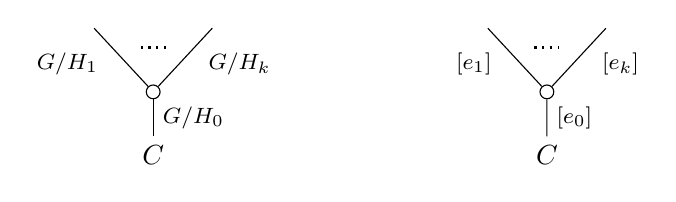
\begin{tikzpicture}
[grow=up,auto,level distance=2.3em,every node/.style = {font=\footnotesize},dummy/.style={circle,draw,inner sep=0pt,minimum size=1.75mm}]
	\node at (0,0) [font=\normalsize]{$C$}
		child{node [dummy] {}
			child{
			edge from parent node [swap,near end] {$G/H_k$} node [name=Kn] {}}
			child{
			edge from parent node [near end] {$G/H_1$}
node [name=Kone,swap] {}}
		edge from parent node [swap] {$G/H_0$}
		};
		\draw [dotted,thick] (Kone) -- (Kn) ;
	\node at (5,0) [font=\normalsize]{$C$}
		child{node [dummy] {}
			child{
			edge from parent node [swap,near end] {$[e_k]$} node [name=Kn] {}}
			child{
			edge from parent node [near end] {$[e_1]$}
node [name=Kone,swap] {}}
		edge from parent node [swap] {$[e_0]$}
		};
		\draw [dotted,thick] (Kone) -- (Kn) ;
\end{tikzpicture}
\]
We will then abbreviate $\sigma^i C = \sigma^{[e_i]} C$, and write $e_i$, $e_i'$ for the two edges of $\sigma^i C $ that degenerate the edge $e_i$ of $C$,
with $e_i$ denoting the inner edge and $e'_i$ the outer
edge.
\[
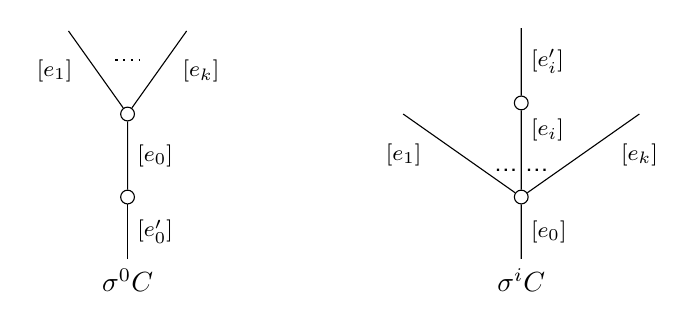
\begin{tikzpicture}
[grow=up,auto,level distance=3em,
every node/.style = {font=\footnotesize},
dummy/.style={circle,draw,inner sep=0pt,minimum size=1.75mm}]
	\node at (0,0) [font=\normalsize]{$\sigma^0 C$}
		child{node [dummy] {}
			child{node [dummy] {}
				child{
				edge from parent node [swap,near end] {$[e_k]$} node [name=Kn] {}}
				child{
				edge from parent node [near end] {$[e_1]$}
node [name=Kone,swap] {}}
			edge from parent node [swap] {$[e_0]$}}
		edge from parent node [swap] {$[e'_0]$}
		};
		\draw [dotted,thick] (Kone) -- (Kn) ;
	\node at (5,0) [font=\normalsize]{$\sigma^i C$}
		child{node [dummy] {}
			child{
			edge from parent node [swap,near end] {$[e_k]$} node [near start,inner sep=1pt,name=Kn] {}}
			child[level distance=3.4em]{node [dummy] {}
				child[level distance=2.7em]{
				edge from parent node [swap] {$[e'_i]$}
}
			edge from parent node [near end,swap] {$[e_i]$}
node [near start,inner sep=1pt,name=Kone,swap] {}
node [near start,inner sep=1pt,name=Kone1] {}}
			child{
			edge from parent node [near end] {$[e_1]$}
node [swap] {}
node [near start,inner sep=1pt,name=Kn1,swap]{}}
		edge from parent node [swap] {$[e_0]$}
		};
		\draw [dotted,thick] (Kone) -- (Kn) ;
		\draw [dotted,thick] (Kone1) -- (Kn1) ;
\end{tikzpicture}
\]
The $G$-tree $\sigma^i C$ then has an orbital inner face\footnote{See \cite[Defn. 2.16]{BP_edss} for a discussion of \textit{orbital} inner faces.}
$\sigma^i C - [e_i]$ obtained by removing $[e_i]$
as well as an orbital outer face obtained by removing $e'_i$,
which we denote $\sigma^i C - [e'_i]$.
Moreover, note that we have natural identifications
$C = \sigma^i C - [e_i]$,
$C = \sigma^i C - [e'_i]$.

In what follows, we will find it convenient to simplify notation by denoting maps $\Omega[T] \to X$,
where $T \in \Omega_G$ and $X \in \mathsf{dSet}^G$,
simply as $T \to X$.


\begin{definition}
	Let $X \in \mathsf{dSet}^G$ be a $G$-$\infty$-operad and $C$ a $G$-corolla with edge orbits
	$[e_0],\cdots,[e_k]$.
	
	Given two parallel operations 
	$f,g\colon C \rightrightarrows X$,
	we write $f \sim_i g$ if there exists a map
	$H \colon \sigma^i C \to X$ such that
\begin{itemize}
\item $f$ equals the restriction $H|_{\sigma^i C-[e'_i]}$;
\item $g$ equals the restriction $H|_{\sigma^i C-[e_i]}$;
\item the restriction $H|_{\sigma^i [e_i]}$
is the degeneracy $\sigma^i [e_i] \to [e_i] \to C \to X$.
\end{itemize}
\end{definition}


\begin{remark}\label{HOMOTBOUND REM}
	Note that if $f \sim_i g$ then it must be
	$f|_{\partial C} = g|_{\partial C}$.
\end{remark}


\begin{example}\label{EQUIVSIM EX}
	Let $G = \mathbb{Z}_{/2} = \{\pm 1\}$
	and consider the $G$-corolla with orbital and expanded representations as given on the left below.
\[
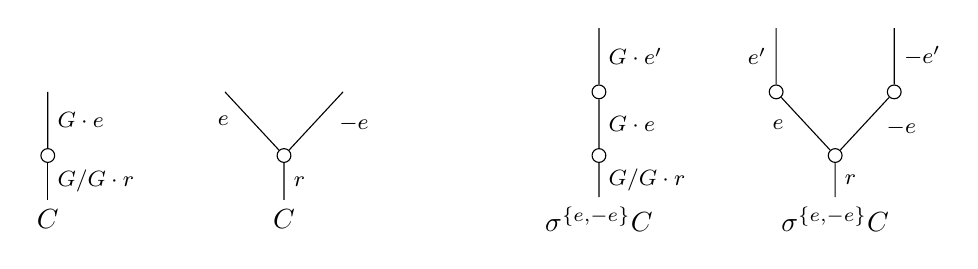
\begin{tikzpicture}
[grow=up,auto,level distance=2.3em,every node/.style = {font=\footnotesize},dummy/.style={circle,draw,inner sep=0pt,minimum size=1.75mm}]
	\node at (0,0) [font=\normalsize]{$C$}
		child{node [dummy] {}
			child{
			edge from parent node [swap] {$G \cdot e$}
node [name=Kone,swap] {}}
		edge from parent node [swap] {$G/G \cdot r$}
		};
	\node at (3,0) [font=\normalsize]{$C$}
		child{node [dummy] {}
			child{
			edge from parent node [swap,near end] {$-e$} node [name=Kn] {}}
			child{
			edge from parent node [near end] {$e$}
node [name=Kone,swap] {}}
		edge from parent node [swap] {$r$}
		};
	\node at (7,0) [font=\normalsize]{$\sigma^{\{e,-e\}} C$}
		child{node [dummy] {}
			child{node [dummy] {}
				child{
				edge from parent node [swap] {$G \cdot e'$}
node [swap] {}}
			edge from parent node [swap] {$G \cdot e$}
node [swap] {}}
		edge from parent node [swap] {$G/G \cdot r$}
		};
	\node at (10,0) [font=\normalsize]{$\sigma^{\{e,-e\}} C$}
		child{node [dummy] {}
			child{node [dummy] {}
				child{
				edge from parent node [swap] {$-e'$} node {}}
			edge from parent node [swap,near end] {$-e$} node {}}
			child{node [dummy] {}
				child{
				edge from parent node {$e'$}
node [swap] {}}
			edge from parent node [near end] {$e$}
node [swap] {}}
		edge from parent node [swap] {$r$}
		};
\end{tikzpicture}
\]
$C$ then has a single leaf $G$-edge orbit $[e] = G \cdot e$, so that for
$f,g \colon C \to X$ it is
$f \sim_1 g$
if there exists a dendrix
$H \colon \sigma^{\{e,-e\}}C \to X$
such that 
\begin{equation}\label{EQUIVHOMOT EQ}
	f = H|_{\sigma^{\{e,-e\}}C - \{e',-e'\}}
\qquad
	g = H|_{\sigma^{\{e,-e\}}C - \{e,-e\}}
\qquad
	H_{\sigma^e e}, H|_{\sigma^{-e}-e} \text{ are degenerate}.
\end{equation}
It is worthwhile to compare this equivariant relation with the relations obtained if one forgets the $G$-actions. Indeed, while \eqref{EQUIVHOMOT EQ} implicitly assumes that all of $f,g,H$ are $G$-equivariant,
by omitting that assumption one can reinterpret 
\eqref{EQUIVHOMOT EQ}
as defining a relation
$f \sim_{[e]} g$ between not necessarily $G$-equivariant maps $f,g \colon C \to X$.

A priori, $\sim_{[e]}$ relation differs from the 
non-equivariant 
$\sim_{e}$ and $\sim_{-e}$
relations obtained by regarding $C$ as a non-equivariant corolla.
However, for $f,g,H$ as in \eqref{EQUIVHOMOT EQ} one has
\begin{equation}\label{EQUIVSIM EQ}
f = H|_{\sigma^{\{e,-e\}}C - \{e',-e'\}}
\sim_e H|_{\sigma^{\{e,-e\}}C - \{e,-e'\}}
\sim_{-e} H|_{\sigma^{\{e,-e\}}C - \{e,-e\}} =g
\end{equation}
so that, by Lemma \ref{EQUIVI LEM}(b) below one has that
$f \sim_{[e]} g$ in fact implies
$f \sim_{e} g$. Moreover, the converse statement follows immediately by using degeneracies.

More generally, similar considerations show that the $\sim$ relations are compatible with restricting the $G$-actions.
\end{example}


\begin{lemma}\label{EQUIVI LEM}
	Let $X \in \mathsf{dSet}^G$ be a $G$-$\infty$-operad and $C$ a $G$-corolla with edge orbits
	$[e_0],\cdots,[e_k]$. Then:
\begin{itemize}
	\item[(a)] each of the relations $\sim_i$ is an equivalence relation;
	\item[(b)] all the equivalence relations $\sim_i$ coincide.
\end{itemize}
\end{lemma}

\begin{proof}
	We first address (a). 
	
	For the reflexive condition, one can take $H$ to be the degeneracy
	$\sigma^i C \xrightarrow{\sigma^i} C \xrightarrow{f} X$.
	
	For the symmetry and transitive conditions, consider the tree
	$\sigma^{ii} C$, which degenerates $[e_i]$ twice.
\[
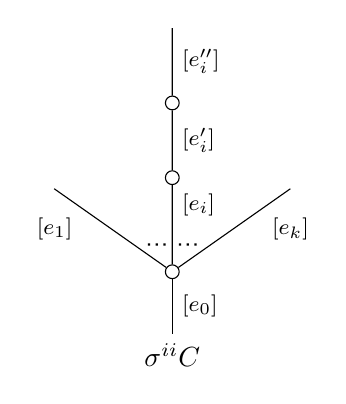
\begin{tikzpicture}
[grow=up,auto,level distance=3em,
every node/.style = {font=\footnotesize},
dummy/.style={circle,draw,inner sep=0pt,minimum size=1.75mm}]
	\node at (0,0) [font=\normalsize]{$\sigma^{ii} C$}
		child{node [dummy] {}
			child{
			edge from parent node [swap,near end] {$[e_k]$} node [near start,inner sep=1pt,name=Kn] {}}
			child[level distance=3.4em]{node [dummy] {}
				child[level distance=2.7em]{node [dummy] {}
					child[level distance=2.7em]{
					edge from parent node [swap] {$[e''_i]$}
}
				edge from parent node [swap] {$[e'_i]$}
}
			edge from parent node [near end,swap] {$[e_i]$}
node [near start,inner sep=1pt,name=Kone,swap] {}
node [near start,inner sep=1pt,name=Kone1] {}}
			child{
			edge from parent node [near end] {$[e_1]$}
node [swap] {}
node [near start,inner sep=1pt,name=Kn1,swap]{}}
		edge from parent node [swap] {$[e_0]$}
		};
		\draw [dotted,thick] (Kone) -- (Kn) ;
		\draw [dotted,thick] (Kone1) -- (Kn1) ;
\end{tikzpicture}
\]
Suppose $f \sim_i g$, and let 
$H \colon \sigma^{i} C \to X$ be the associated homotopy.
Define a map 
$\bar{H} \colon \Lambda^{[e_i]}_o[\sigma^{ii} C] \to X$ by
\[
	\bar{H}|_{\sigma^{ii}C - [e''_i]} = H,
		\qquad
	\bar{H}|_{\sigma^{ii}C - [e'_i]} = f \circ \sigma^i,
		\qquad
	\bar{H}|_{\sigma^{ii} [e_i]} = 
	f|_{[e_i]} \circ \sigma^{ii} =
	g|_{[e_i]} \circ \sigma^{ii}.
\]
Since the orbital inner horn inclusion
$\bar{H} \colon \Lambda^{[e_i]}_o[\sigma^{ii} C] \to \Omega[C]$
is $G$-inner anodyne by \cite[Prop. 3.13]{BP_edss},
$\bar{H}$ admits an extension $\widetilde{H} \colon \sigma^{ii}C \to X$.
The restriction $\bar{H}|_{\sigma^{ii}C - [e_i]}$ then provides the homotopy exhibiting $g \sim_i f$, and symmetry of $\sim_i$ follows.

Next, suppose $f \sim_i g$ and $g \sim_i h$, and let 
$H \colon \sigma^{i} C \to X$ and
$K \colon \sigma^{i} C \to X$ be be the associated homotopies.
Define a map 
$\bar{H} \colon \Lambda^{[e'_i]}_o[\sigma^{ii} C] \to X$ by
\[
	\bar{H}|_{\sigma^{ii}C - [e''_i]} = H,
		\qquad
	\bar{H}|_{\sigma^{ii}C - [e_i]} = K,
		\qquad
	\bar{H}|_{\sigma^{ii} [e_i]} = 
	f|_{[e_i]} \circ \sigma^{ii} =
	g|_{[e_i]} \circ \sigma^{ii} =
	h|_{[e_i]} \circ \sigma^{ii}.
\]
$\bar{H}$ again admits an extension $\widetilde{H} \colon \sigma^{ii}C \to X$, and the restriction $\bar{H}|_{\sigma^{ii}C - [e'_i]}$
provides the homotopy exhibiting $f \sim_i g$, so that transitivity of $\sim_i$.

We next turn to (b). Consider the tree $\sigma^{ij} C$ which degenerates $C$ once along each of $[e_i]$ and $[e_j]$.
\[
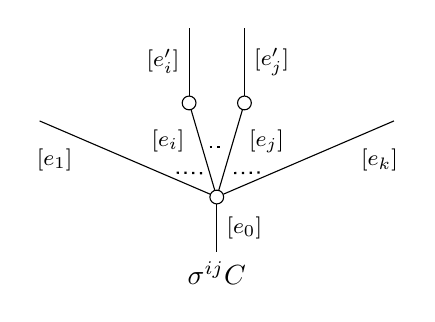
\begin{tikzpicture}
[grow=up,auto,level distance=2.75em,
every node/.style = {font=\footnotesize},
dummy/.style={circle,draw,inner sep=0pt,minimum size=1.75mm}]
	\node at (0,0) [font=\normalsize]{$\sigma^{ij} C$}
		child{node [dummy] {}
			child{
			edge from parent node [swap,near end] {$[e_k]$} node [near start,inner sep=1pt,name=Kn] {}}
			child[level distance=3.4em,sibling distance=2em]{node [dummy] {}
				child[level distance=2.7em]{
				edge from parent node [swap] {$[e'_j]$}
}
			edge from parent node [very near end,swap] {$[e_j]$}
node [near start,inner sep=1pt,name=Kone,swap] {}
node [inner sep=1pt,name=Kn2] {}}
			child[level distance=3.4em,sibling distance=2em]{node [dummy] {}
				child[level distance=2.7em]{
				edge from parent node {$[e'_i]$}
}
			edge from parent node [very near end] {$[e_i]$}
node [inner sep=1pt,name=Kone2,swap] {}
node [near start,inner sep=1pt,name=Kone1] {}}
			child{
			edge from parent node [near end] {$[e_1]$}
node [swap] {}
node [near start,inner sep=1pt,name=Kn1,swap]{}}
		edge from parent node [swap] {$[e_0]$}
		};
		\draw [dotted,thick] (Kn) -- (Kone) ;
		\draw [dotted,thick] (Kone1) -- (Kn1) ;
		\draw [dotted,thick] (Kone2) -- (Kn2) ;
\end{tikzpicture}
\]
Suppose $f \sim_i g$ with $H \colon \sigma^{i} C \to X$ the associated homotopy.
Define a map 
$\bar{H} \colon \Lambda^{[e_i]}_o[\sigma^{ij} C] \to X$ by
\[
	\bar{H}|_{\sigma^{ij}C - [e'_j]} = H,
		\qquad
	\bar{H}|_{\sigma^{ij}C - [e_j]} = f \circ \sigma^i,
		\qquad
	\bar{H}|_{\sigma^{ij}C - [e'_i]} = f \circ \sigma^j.
\]
Yet again, $\bar{H}$ admits an extension $\widetilde{H} \colon \sigma^{ij}C \to X$, and the restriction $\bar{H}|_{\sigma^{ij}C - [e_i]}$
provides a homotopy exhibiting $g \sim_j f$. (b) now follows.
\end{proof}

In light of Lemma \ref{EQUIVI LEM},
given parallel operation $f,g \colon C \rightrightarrows X$ with 
$C$ a $G$-corolla and $X$ a $G$-$\infty$-operad,
we will henceforth write $f \sim g$ whenever $f \sim_i g$ for some (and thus all) $i$.
We now extend the $\sim$ relation.

\begin{definition}\label{XTENDSIM DEF}
	Let $T \in \Omega_G$ be a $G$-tree
	and $X \in \mathsf{dSet}^G$ be a 
	$G$-$\infty$-operad.
	
	Given dendrices $x,y\colon T \to X$ we write
	$x \sim y$ if there are equivalences of restrictions
	$x|_{T_v} \sim y|_{T_v}$ for all $G$-vertices
	$v \in \boldsymbol{V}_G(T)$.
	
	Further, we define $\mathsf{ho}(X)(T) = X(T)/\sim$.
\end{definition}

\begin{proposition}
Let $X \in \mathsf{dSet}^G$ be a $G$-$\infty$-operad. Then the assignment 
		$T \mapsto \mathsf{ho}(X)(T)$
		is a contravariant functor in $T \in \Omega_G$, i.e.
		$\mathsf{ho}(X)\in \mathsf{dSet}_G$.
\end{proposition}


\begin{proof}
	It suffices to show that the $\sim$ equivalence relations are compatible with the generating classes of maps in $\Omega_G$, namely
	degeneracies, inner faces, outer faces, and quotient maps.
	
	The cases of degeneracies and outer faces are obvious. In the case of quotients, 
	since any quotient $\bar{T} \to T$ of $G$-trees induces quotients on $G$-vertices, it suffices to consider the case of a quotient
	$\bar{C} \xrightarrow{\pi} C$ of $G$-corollas.
	But it is then straightforward to check that if a homotopy exhibiting $f \sim_0 g$ also induces a homotopy exhibiting 
	$f \circ \pi \sim_0 g \circ \pi$
	(notably, the same needs not be true for the relations $f \sim_i g$ when $0<i$, 
	in which case the exhibiting homotopy 
	may instead exhibit a string of relations 
	$f \circ \pi \sim \cdots \sim g \circ \pi$
	as in \eqref{EQUIVSIM EQ}).

It remains to address the most interesting case,
that inner faces. Since inner faces can be factored as composites of inner faces that collapse a singe inner edge orbit,
it suffices to consider the case of faces
$D \to T$ where $T$ has a single inner edge orbit; that is,
we can assume that there are $G$-corollas
$C_1$, $C_2$ such that 
$T = C_1 \amalg_{[e_i]} C_2$ and
$D = T - [e_i]$, as illustrated below.
\[
\begin{tikzpicture}
[grow=up,auto,level distance=3em,
every node/.style = {font=\footnotesize},
dummy/.style={circle,draw,inner sep=0pt,minimum size=1.75mm}]
	\node at (0,0) [font=\normalsize]{$C_1$}
		child{node [dummy] {}
			child{
			edge from parent node [swap,near end] {} node [near start,inner sep=1pt,name=Kn] {}}
			child[level distance=3.4em]{node {}
			edge from parent node [near end,swap] {$[e_i]$}
node [near start,inner sep=1pt,name=Kone,swap] {}
node [near start,inner sep=1pt,name=Kone1] {}}
			child{
			edge from parent node [near end] {}
node [swap] {}
node [near start,inner sep=1pt,name=Kn1,swap]{}}
		edge from parent node [swap] {$[e_0]$}
		};
		\draw [dotted,thick] (Kone) -- (Kn) ;
		\draw [dotted,thick] (Kone1) -- (Kn1) ;
	\node at (4,0) [font=\normalsize]{$C_2$}
		child{node [dummy] {}
			child{
			edge from parent node [swap,near end] {} node [name=Kn] {}}
			child{
			edge from parent node [near end] {}
node [name=Kone,swap] {}}
		edge from parent node [swap] {$[e_i]$}
		};
		\draw [dotted,thick] (Kone) -- (Kn) ;
	\node at (9,0) [font=\normalsize]{$T$}
		child{node [dummy] {}
			child{
			edge from parent node [swap,near end] {} node [near start,inner sep=1pt,name=Kn] {}}
			child[level distance=3.4em]{node [dummy] {}
				child{
				edge from parent node [swap,near end] {} node [name=Kn2] {}}
				child{
				edge from parent node [near end] {}
node [name=Kone2,swap] {}}
			edge from parent node [near end,swap] {$[e_i]$}
node [near start,inner sep=1pt,name=Kone,swap] {}
node [near start,inner sep=1pt,name=Kone1] {}}
			child{
			edge from parent node [near end] {}
node [swap] {}
node [near start,inner sep=1pt,name=Kn1,swap]{}}
		edge from parent node [swap] {$[e_0]$}
		};
		\draw [dotted,thick] (Kone) -- (Kn) ;
		\draw [dotted,thick] (Kone1) -- (Kn1) ;
		\draw [dotted,thick] (Kone2) -- (Kn2) ;
\end{tikzpicture}
\]
The claim is now that if
$x,y \colon T \to X$ are such that
$x|_{C_1} \sim y|_{C_1}$ and
$x|_{C_2} \sim y|_{C_2}$
then it is also 
$x|_{D} \sim y|_{D}$.
This will follow from the next two claims:
\begin{itemize}
\item[(i)] if $x,y \colon T \to X$ are such that
$x|_{C_1} = y|_{C_1}$ and
$x|_{C_2} = y|_{C_2}$
then $x|_{D} \sim y|_{D}$;
\item[(ii)]
given $x \colon T \to X$, $f\colon C_1 \to X$ and
$g \colon C_2 \to X$ such that
$f \sim x|_{C_1}$, $g \sim x|_{C_2}$,
there exists
$y \colon T \to X$ such that
$y|_{C_1} = f$, $y|_{C_2} = g$ and
$y|_D = x|_D$.
\end{itemize}
To show (i) and (ii), consider the degeneracies
$\sigma^0 T$ and $\sigma^i T$ pictured below.
\[
\begin{tikzpicture}
[grow=up,auto,level distance=3em,
every node/.style = {font=\footnotesize},
dummy/.style={circle,draw,inner sep=0pt,minimum size=1.75mm}]
	\node at (0,0) [font=\normalsize]{$\sigma^0 T$}
		child{node [dummy] {}
		child{node [dummy] {}
			child{
			edge from parent node [swap,near end] {} node [near start,inner sep=1pt,name=Kn] {}}
			child[level distance=3.4em]{node [dummy] {}
				child{
				edge from parent node [swap,near end] {} node [name=Kn2] {}}
				child{
				edge from parent node [near end] {}
node [name=Kone2,swap] {}}
			edge from parent node [near end,swap] {$[e_i]$}
node [near start,inner sep=1pt,name=Kone,swap] {}
node [near start,inner sep=1pt,name=Kone1] {}}
			child{
			edge from parent node [near end] {}
node [swap] {}
node [near start,inner sep=1pt,name=Kn1,swap]{}}
		edge from parent node [swap] {$[e_0]$}}
		edge from parent node [swap] {$[e'_0]$}
		};
		\draw [dotted,thick] (Kone) -- (Kn) ;
		\draw [dotted,thick] (Kone1) -- (Kn1) ;
		\draw [dotted,thick] (Kone2) -- (Kn2) ;
	\node at (6,0) [font=\normalsize]{$\sigma^i T$}
		child{node [dummy] {}
			child{
			edge from parent node [swap,near end] {} node [near start,inner sep=1pt,name=Kn] {}}
			child[level distance=3.4em]{node [dummy] {}
			child{node [dummy] {}
				child{
				edge from parent node [swap,near end] {} node [name=Kn2] {}}
				child{
				edge from parent node [near end] {}
node [name=Kone2,swap] {}}
			edge from parent node [swap] {$[e'_i]$}}
			edge from parent node [near end,swap] {$[e_i]$}
node [near start,inner sep=1pt,name=Kone,swap] {}
node [near start,inner sep=1pt,name=Kone1] {}}
			child{
			edge from parent node [near end] {}
node [swap] {}
node [near start,inner sep=1pt,name=Kn1,swap]{}}
		edge from parent node [swap] {$[e_0]$}
		};
		\draw [dotted,thick] (Kone) -- (Kn) ;
		\draw [dotted,thick] (Kone1) -- (Kn1) ;
		\draw [dotted,thick] (Kone2) -- (Kn2) ;
\end{tikzpicture}
\]
Given $x,y$ as in (i), one can now build a map
$H \colon \Lambda_o^{[e_i]}[\sigma^0 T] \to X$ by
\[
	H|_{\sigma^0 T - [e_0]} = x,
\qquad
	H|_{\sigma^0 T - [e'_0]} = y,
\qquad
	H|_{\sigma^0 C_1} = 
	x|_{C_1} \circ \sigma^0 = 
	y|_{C_1} \circ \sigma^0.
\]
Letting $\widetilde{H}\colon \sigma^0 T \to X$
be an extension of $H$,
the restriction $H|_{\sigma^0 T - [e_i]}$
provides the desired homotopy 
$x|_{D} \sim y|_{D}$, showing (i).


Lastly, let $x,f,g$ be as in (ii), 
and let
$K \colon \sigma^i C_1 \to X$ exhibit the relation
$f \sim_i x|_{C_1}$
and 
$ \bar{K} \colon \sigma^i C_2 \to X$
exhibit the relation
$x|_{C_2} \sim_i g$ (note the reversed order).
Now build the map
$H \colon \Lambda_o^{[e'_i]}[\sigma^i T] \to X$ by
\[
	H|_{\sigma^i T - [e_i]} = x,
\qquad
	H|_{\sigma^i C_1} = K,
\qquad
	H|_{\sigma^i C_2} = \bar{K}.
\]
Again letting 
$\widetilde{H} \colon \sigma^i T \to X$,
the restriction 
$\widetilde{H}|_{\sigma^i T - [e'_i]}$
provides the required $y \colon T \to X$,
showing (ii) and finishing the proof.
\end{proof}


\begin{corollary}\label{HOOPUNIV COR}
Let $X \in \mathsf{dSet}^G$ be a $G$-$\infty$-operad. Then
	\begin{itemize}
	\item[(a)] $\mathsf{ho}(X)\in \mathsf{dSet}_G$ is a genuine equivariant operad, i.e. it satisfies the strict right lifting condition against the Segal core inclusions
	$Sc[T] \to \Omega[T]$ for $T \in \Omega_G$;
	\item[(b)] the quotient map
	$\upsilon_{\**}X \to \mathsf{ho}(X)$ is the universal map from $\upsilon_{\**}X$ to a genuine equivariant operad.
	\end{itemize}
\end{corollary}

\begin{proof}
	Note first that by Remark \ref{HOMOTBOUND REM}
	any map 	$Sc[T] \to \mathsf{ho}(X)$ admits a factorization 
	$Sc[T] \to \upsilon_{\**}X \xrightarrow{q} \mathsf{ho}(X)$.
	
	The right lifting property for $\mathsf{ho}(X)$
	against the maps $Sc[T] \to \Omega[T]$
	is then automatic from the lifting property for $X$.

	For strictness,	
	note that Definition \ref{XTENDSIM DEF}
	can be reinterpreted as saying that
	a pair of dendrices $\Omega[T] \rightrightarrows X$
	give rise to the same point of 
	$\mathsf{ho}(X)$, i.e. 
	the composites 
	$\Omega[T] \rightrightarrows X \xrightarrow{q}
	\mathsf{ho}(X)$ coincide, 
	iff the composites 
	$Sc[T] \to \Omega[T] \rightrightarrows X \xrightarrow{q}
	\mathsf{ho}(X)$ coincide, showing strictness, and thus (a).
		
	For (b), since $\mathsf{ho}(X)$ is a quotient of
	$\upsilon_{\**} X$, it suffices to show that any map
	from $F \colon \upsilon_{\**}X \to Y$ with $Y$ a genuine equivariant operad must also enforce the $\sim$ relation.
	For a $G$-corolla $C$ and
	$f,g\colon C \to X$ such that 
	$H \colon \sigma^i C \to X$ exhibits
	$f \sim_i g$, 
	the strict lifting condition for $Y$
	shows that the maps
	$F\circ H \colon \sigma^i C \to Y$,
	$f \circ \sigma^i \colon \sigma^i C \to Y$
	must coincide, and thus that
	$F(f)=F(g)$.
	The further claim that $F$ respects equivalences
	of general pair of dendrices $T \rightrightarrows X$
	is immediate from Definition \ref{XTENDSIM DEF}.
\end{proof}



{\color{red} HERE}

The following is the analogue of \cite[Prop. 4.8]{CM13b}.

\begin{proposition}
      \label{HOOPID_PROP}
Let $\mathcal{O} \in \mathsf{sOp}^G$
be a fibrant. 
Then there is a natural isomorphism of genuine equivariant operads
\begin{equation}\label{HOOPID EQ}
ho(hcN(\mathcal{O})) \xrightarrow{\simeq}
\pi_0 \left( \upsilon_{\**} N\mathcal{O} \right).
\end{equation}
\end{proposition}


\begin{proof}
      By \cite[Prop. 5.9]{BP_edss}, $\pi_0(\upsilon_{\**}N\O)$ is a genuine equivariant operad,
      and the existence of the map in \eqref{HOOPID EQ}
      will be an application of
      Corollary \ref{HOOPUNIV COR}(b).

Firstly,
note that we have the following, naturally in $T \in \Omega_G$.
\[
\upsilon_{\**}hcN(\O)(T)
\simeq
\mathsf{sOp}^G(W_!\Omega[T],\O)
\simeq
\mathsf{sdSet}^G(N W_!\Omega[T],N \O)
\simeq 
\mathsf{sdSet}_G(\upsilon_{\**}N W_!\Omega[T],\upsilon_{\**}N \O)
\]
where the second and third identifications use the fact that 
$N\colon \mathsf{Op} \to \mathsf{dSet}$ and $\upsilon_{\**} \colon \dSet^G \to \dSet_G$
are fully faithful inclusions. 
But now one has a map
\begin{align*}
  \mathsf{sdSet}_G(\upsilon_{\**}N W_!\Omega[T],\upsilon_{\**}N \O)
  & \to
    \mathsf{sdSet}_G(\upsilon_{\**}N W_!\Omega[T],\pi_0\upsilon_{\**}N \O)
  \\ & \simeq
       \mathsf{dSet}_G(\pi_0 \upsilon_{\**}  N W_!\Omega[T],\pi_0\upsilon_{\**}N \O)
  \\ & \simeq
       \mathsf{dSet}_G(\upsilon_{\**}\Omega[T],\pi_0\upsilon_{\**}N \O)
  \\ & =
       (\pi_0\upsilon_{\**}N \O)(T)
\end{align*}
so altogether we obtain a map
$\upsilon_{\**}hcN(\O) \to \pi_0 \upsilon_{\**} N \O$
and hence, by Corollary \ref{HOOPUNIV COR},
the desired map 
\[ho(hcN(\O)) \to \pi_0 \upsilon_{\**} N \O\]
Moreover, both of these are quotients of $\upsilon_{\**}hcN(\O)$,
so to prove that the map is an isomorphism one needs only show that any two parallel operations $C \rightrightarrows hcN \O$ of $\upsilon_{\**}hcN(\O)$
that are identified in 
$\pi_0 \upsilon_{\**} N \O$
were already identified in 
$ho(hcN(\O))$.
But this now follows immediately from the pushout from Proposition \ref{WLEFTQPUSH PROP}
\[
\begin{tikzcd}
	\Omega(C) \otimes_{\mathsf{F}}
	\partial \Delta[1]
	\ar{r} \ar{d}
&
	W_! \left(\partial \Omega[C \star \eta]\right) 
	\ar{d}
\\
	\Omega(C) \otimes_{\mathsf{F}}
	\Delta[1]
	\ar{r}
&
	W(C \star \eta)
\end{tikzcd}
\]
\end{proof}


come back

\begin{lemma}
      $ho(X)$ detects isofibrations between $\F$-$\infty$-operads.
\end{lemma}
\begin{proof}
      Consider the composite
      \[
            \Op^G_\infty \xrightarrow{ho}
            \dSet_G \xrightarrow{k^{\**}}
            \dSet^{\mathsf O_{\F_1}^{op}} \xrightarrow{j^{\**}}
            \sSet^{\mathsf O_{\F_1}^{op}} \xrightarrow{\tau}
            \Cat^{\mathsf O_{\F_1}^{op}}
      \]
      for $k \colon \Omega \times \mathsf O_{\F_1} \to \Omega_G$.
      Since $ho(X)$ is strict Segal, so is $(kj)^{\**} ho(X)$. % and thus $N\tau j^{\**}ho(X) = j^{\**}ho(X)$.
      Moreover, as $(kj)^{\**} \upsilon_{\**} X \to (kj)^{\**} ho(X)$ is again universal to a strict Segal object,
      the universal property of the unit map implies that
      \[
            (kj)^{\**}ho(X) = N \tau (kj)^{\**} ho(X) \simeq N \tau (kj)^{\**} \upsilon_{\**} X
      \]
      where the first equality is from the strict Segal property.
      Finally, $f \colon X \to Y$ in $\dSet^G$ is an isofibration iff $\tau j^{\**}(f^H)$ is for each $H \in \F_1$,
      or equivalently if $\tau (kj)^{\**} \upsilon_{\**} f$ is a level isofibration.
      The result follows.
\end{proof}

\begin{remark}
      \label{W!_LEFTQ_REM}
      This gives us a second finish to the proof of Proposition \ref{W!_LEFTQ_PROP}:
      $hcN(f)$ is an $\F$-fibration iff $\tau (kj)^{\**} \upsilon_{\**} h c N(f)$ is,
      but
      \[
            +            \tau (kj)^{\**} \upsilon_{\**} hcN(f) =
            \tau N \tau (kj)^{\**} \upsilon_{\**} hcN(f) \simeq
            \tau (kj)^{\**} ho( hcN(f) ) \simeq
            \tau (kj)^{\**} \pi_0 \upsilon_{\**} N \O =
            \pi_0 j^{\**} i_{\**} f,
      \]
      where the last equality follows from the diagram below.
      \[
            \begin{tikzcd}[column sep = scriptsize]
                  \sOp^G \arrow[d, equal] \arrow[rrr, "i_{\**}"]
                  &&&
                  \sOp^{\mathsf O_{\F_1}^{op}} \arrow[d, "N"'] \arrow[r, "j^{\**}"]
                  &
                  \mathsf{sCat}^{\mathsf O_{\F_1}^{op}} \arrow[d, "N"'] \arrow[r, "\pi_0"]
                  &
                  \Cat^{\mathsf O_{\F_1}^{op}} \arrow[d, "N"'] \arrow[r, equal]
                  &
                  \Cat^{\mathsf O_{\F_1}^{op}} \arrow[d, equal]
                  \\
                  \sOp^G \arrow[d, equal] \arrow[r, "N"]
                  &
                  \mathsf{sdSet}^G \arrow[d, equal] \arrow[rr, "i_{\**}"]
                  &&
                  \mathsf{sdSet}^{\mathsf O_{\F_1}^{op}} \arrow[d, equal] \arrow[r, "j^{\**}"]
                  &
                  \mathsf{ssSet}^{\mathsf O_{\F_1}^{op}} \arrow[r, "\pi_0"]
                  &
                  \sSet^{\mathsf O_{\F_1}^{op}} \arrow[d, equal] \arrow[r, "\tau"]
                  &
                  \Cat^{\mathsf O_{\F_1}^{op}} \arrow[d, equal]
                  \\
                  \sOp^G \arrow[d, equal] \arrow[r, "N"]
                  &
                  \mathsf{sdSet}^G \arrow[d, equal] \arrow[r, "\upsilon_{\**}"]
                  &
                  \mathsf{sdSet}_G \arrow[d, equal] \arrow[r, "k^{\**}"]
                  &
                  \mathsf{sdSet}^{\mathsf O_{\F_1}^{op}} \arrow[r, "\pi_0"]
                  &
                  \dSet^{\mathsf O_{\F_1}^{op}} \arrow[d, equal] \arrow[r, "j^{\**}"]
                  &
                  \sSet^{\mathsf O_{\F_1}^{op}} \arrow[d, equal] \arrow[r, "\tau"]
                  &
                  \Cat^{\mathsf O_{\F_1}^{op}} \arrow[d, equal]
                  \\
                  \sOp^G \arrow[r, "N"]
                  &
                  \mathsf{sdSet}^G \arrow[r, "\upsilon_{\**}"]
                  &
                  \mathsf{sdSet}_G \arrow[r, "\pi_0"]
                  &
                  \dSet_G \arrow[r, "k^{\**}"]
                  &
                  \dSet^{\mathsf O_{\F_1}^{op}} \arrow [r, "j^{\**}"]
                  &
                  \sSet^{\mathsf O_{\F_1}^{op}} \arrow[r, "\tau"]
                  &
                  \Cat^{\mathsf O_{\F_1}^{op}}
            \end{tikzcd}
      \]
      But $f \in \sOp^G$ is an isofibration iff
      $\pi_0 j^{\**} i_{\**} f$ is a level isofibration, finishing the proof.
\end{remark}














\section{For the sequel?}



\begin{example}
	\label{FREEOP_EX}
	We unpack these definitions with several examples.
	\begin{enumerate}[label = (\roman*)]
		\item With $n = 0$, we see $\mathbb F_H[\varnothing] = G/H \cdot \Omega(\eta)$ is cofibrant for all $H \in \mathcal F_0$.
		\item With $n = 1$ and $\Gamma = H \leq G \simeq G \times \Sigma_1$, $\mathfrak C_\Gamma = G/H \cdot \set{0,1}$, and
		\[
		\mathbb F_{\Gamma}[\varnothing] = G/H \cdot (\set{0,1} \cdot \Omega(\eta)),
		\qquad
		\mathbb F_{\Gamma}[1_\V] = G/H \cdot \mathbb A^{op} = \Omega(G/H \cdot C_1).
		\]
		with two orbits of objects and a single orbit of non-trivial hom-objects in the latter case.
		\item For higher arity operations,
		if $\Gamma \leq G \times \Sigma_n$ is a \textit{graph subgroup}, i.e. the graph of a homomorphism $G \geq H \xrightarrow{\alpha} \Sigma_n$, then
		we have an identification $\mathfrak C_{\Gamma} \simeq G \cdot_H (A_+)$ where $A$ denotes $n$ equipped with the $H$-action provided by $\alpha$.
		Morevover, if $C = C_A \in \Sigma_G$ is the $G$-corolla (unique up to isomorphism) corresponding to the graph subgroup $\Gamma$, then
		\[
		\mathbb F_\Gamma[\varnothing] = \partial\Omega(C) = \coprod_{Ge \in \boldsymbol{E}_G(C)} Ge \cdot \Omega(\eta),
		\qquad
		\mathbb F_{\Gamma}[1_\V] = \Omega(C),
		\qquad
		\mathbb F_\Gamma[\Gamma/\Gamma \cdot K] = \Omega(C) \otimes_\Fin K,
		\]
		with $K \in \V$ and $\otimes_\Fin$ denotes the $\V$-tensoring from Example \ref{TENS_EX};
		in this case, we note that the tensoring is levelwise, with
		$(\Omega(C) \otimes_\Fin K)(\vect C) = \Omega(C)(\vect C) \otimes K$.            
		
		In particular, we conclude that $\Omega(C) \in \Op^G_\bullet(\V)$ is cofibrant for all $C \in \Sigma_G$ via the following factorization.
		\[
		\varnothing \to \partial \Omega(C) \xrightarrow{\mathbb F_{\Gamma}(\varnothing \to 1_\V)} \Omega(C).
		\]
		\todo[inline]{connect to Definition \ref{OT_DEF}}
		\item Similarly, $\Omega(T) \in \Op^G_\bullet(\V)$ is cofibrant for all $T \in \Omega_G$, as
		the grafting decompositions $T = C \coprod_{\boldsymbol{E}_G(C)} (T_{Ge})$ induces the following pushout in $\Op^G_\bullet(\V)$.
		\[
		\begin{tikzcd}
		\displaystyle{
			\coprod_{Ge \in \boldsymbol{E}_G(C)} \Omega(Ge)}
		\arrow[r] \arrow[d]
		&
		\Omega(C) \arrow[d]
		\\
		\displaystyle{
			\coprod_{Ge \in \boldsymbol{E}_G(C)} \Omega(T_e)}
		\arrow[r]
		&
		\Omega(T)
		\end{tikzcd}
		\]            
		\todo[inline]{$\Omega(T)$ is $\mathcal F$-cofibrant iff $T \in \Omega_{\mathcal F}$}
	\end{enumerate}
\end{example}


\begin{remark}
	Following Example \ref{FREEOP_EX}, we see that
	when $\F = \F^\Gamma$ is the is the $(G, \Sigma)$-family of graph subgroups,
	generating cofibrations and trivial cofibrations of $\Op^G_{\F^\Gamma}(\sSet)$ are, respectively, 
	\begin{gather*}
	\set{\Omega(C) \otimes_\Fin(\partial \Delta[n] \to \Delta[n])}_{C \in \Sigma_G, n \geq 0} \bigcup 
	\set{G/H \cdot (\varnothing \to \Omega(\eta))}_{H \leq G}
	\stepcounter{equation}\tag{\theequation}\label{SSETGENCOF_EQ}
	\\
	\set{\Omega(C) \otimes_\Fin(\Lambda^i[n] \to \Delta[n])}_{C \in \Sigma_G, 0 \leq i \leq n} \bigcup
	\set{G/H \cdot (\Omega(\eta) \to \mathbb J)}_{H \leq G, \mathbb J \in \mathscr G}.
	\end{gather*}     
\end{remark}













\subsubsection*{Underlying cofibrancy in $\Op^G_{\mathfrak C}(\sSet)$}

We end this section by specifying to $\V = \sSet$ and determining a characterization of $\Sigma_{\F^\Gamma}$-cofibrant operads.
First, we recall the notion of a $G$-graph subgroup (e.g. \cite[Defn. 6.34]{BP_geo}).
\begin{definition}
      \label{GRAPHSUB_DEF}
      A subgroup $\Gamma \leq G \times \Sigma_n^{op}$ is called a \textit{$G$-graph subgroup} if
      $\Gamma \cap \Sigma_n^{op} = \**$.
      Equivalently, $\Gamma$ is of the form $\set{(h, \alpha(h)^{-1})}$ for $h \in H$ for some subgroup $H \leq G$ and $\alpha \colon H \to \Sigma_n$ a homomorphism.

      Let $\F_n^\Gamma$ denote the family of $G$-graph subgroups of $G \times \Sigma_n$, and $\F^\Gamma = \set{\F_n^{\Gamma}}$ the $(G,\Sigma)$-family of $G$-graph subgroups.
      More generally, we call any subfamily of $\F^{\Gamma}$ a \textit{$(G,\Sigma)$-graph family}\footnote{These have previously been called \textit{families of $G$-corollas} \cite[Defn. 4.44]{BP_geo} and \textit{$G$-vertex families} \cite[Defn. 9.3]{Per18}.}.
\end{definition}

Now, recall (e.g. \cite[Prop. 2.16]{Ste16}) that for any group $G$ and family of subgroups $\F$,
$K \to L$ in $\sSet^{G}_\F$ is an $\F$-cofibration iff $L_n \setminus K_n$ has isotropy in $\F$; i.e. for all $x \in L_n \setminus K-n$, $\Stab_{G}(x) \in \F$. 
% 
We also note the easy observation that for any set $A$ with an action of $G \times \Sigma$,
$A$ has isotropy in the family $\F^\Gamma$ of $G$-graph subgroups
iff
$A$ is $\Sigma$-free.
% 
Thus $K \to L$ in $\sSet^{G \times \Sigma}_{\F^\Gamma}$ is an $\F^\Gamma$-cofibration
iff
it forgets to a cofibration in the coarse model structure $\sSet^\Sigma_{proj}$.

More generally, if $\Lambda \leq G \times \Sigma$ and $\F^\Gamma_{\Lambda} = \F^\Gamma \cap \Lambda$,
then $K \to L$ in $\sSet^{\Lambda}_{\F^\Gamma_\Lambda}$ is an $\F^\Gamma_\Lambda$-cofibration
iff
it forgets to a cofibration in the coarse model structure $\sSet^{\pi_{\Sigma}\Lambda}_{proj}$.
      
All together, we conclude the following (cf. \cite[Remark 6.7]{Per18}, \cite[discussion before Thm. 2.31]{BP_edss}).

\begin{proposition}
      \label{SGS_COF_PROP}
      $\O \to \P$ in $\Op_\bullet^G(\sSet)$ is a $\Sigma_{\F^\Gamma}$-cofibration iff
      it forgets to a $\Sigma$-cofibration in $\Op_\bullet(\sSet)$
      (i.e. it forgets to a cofibration in $\Sym_\bullet(\sSet)$).
      %
      Equivalently, $\O$ is $\Sigma_{\F^\Gamma}$-cofibrant iff $\O(n)$ has a free $\Sigma_n$-action.
\end{proposition}








\newpage

\bibliography{biblio3}{}
\bibliographystyle{amsalpha2}



\end{document}


%%% Local Variables:
%%% mode: latex
%%% TeX-master: t
%%% End:
